\documentclass[ALICE,manyauthors]{ALICE_analysis_notes}
%
%particles
\newcommand{\jpsi}{\rm J/$\psi$}
\newcommand{\psip}{$\psi^\prime$}
\newcommand{\jpsiDY}{\rm J/$\psi$\,/\,DY}
\newcommand{\chic}{$\chi_{\rm c}$}
\newcommand{\pip}{$\pi^{+}$}
\newcommand{\pim}{$\pi^{-}$}
\newcommand{\pizero}{$\pi^{0}$}
\newcommand{\kap}{K$^{+}$}
\newcommand{\kam}{K$^{-}$}
\newcommand{\pbar}{$\rm\overline{p}$}
\newcommand{\ccbar}{\ensuremath{\mathrm{c\overline{c}}}}
\newcommand{\bbbar}{\ensuremath{\mathrm{b\overline{b}}}}
\newcommand{\Dzero}{\ensuremath{\mathrm{D^{0}}}}
\newcommand{\Dzerobar}{\ensuremath{\mathrm{\overline{D^{0}}}}}
\newcommand{\Dpm}{\ensuremath{\mathrm{D^{\pm}}}}
\newcommand{\Ds}{\ensuremath{\mathrm{D_{s}^{\pm}}}}
\newcommand{\Dstar}{\ensuremath{\mathrm{D^{*\pm}}}}

%collision systems
\newcommand{\pp}{pp}
\newcommand{\pPb}{p--Pb}
\newcommand{\PbPb}{Pb--Pb}

%detectors
\newcommand{\ezdc}{$E_{\rm ZDC}$}

%units
\newcommand{\GeVc}{\ensuremath{{\rm GeV/}c}}
\newcommand{\GeVcsq}{\ensuremath{{\rm GeV/}c^2}}

%others
\newcommand{\degree}{$^{\rm o}$}
\newcommand{\s}{\ensuremath{\sqrt{s}}}
\newcommand{\snn}{\ensuremath{\sqrt{s_{\rm NN}}}}
\newcommand{\y}{\ensuremath{y}}
\newcommand{\pt}{\ensuremath{p_{\rm T}}}
\newcommand{\dedx}{d$E$/d$x$}
\newcommand{\dndy}{d$N$/d$y$}
\newcommand{\dndydpt}{${\rm d}^2N/({\rm d}y {\rm d}\pt)$}
\newcommand{\dndetadpt}{\ensuremath{{\rm d}^2N/({\rm d}\eta {\rm d}\pt)}}
\newcommand{\dsigmadetadpt}{\ensuremath{{\rm d}^2\sigma/({\rm d}\eta {\rm d}\pt)}}
\newcommand{\dndpt}{d$N$/d\pt}
\newcommand{\zpar}{\ensuremath{z_{||}}}
\newcommand{\zpargen}{\ensuremath{z_{||}^{\mathrm{part}}}}
\newcommand{\zpardet}{\ensuremath{z_{||}^{\mathrm{det}}}}
\newcommand{\ptchjet}{\ensuremath{p_{\mathrm{T,ch\, jet}}}}
\newcommand{\ptjet}{\ensuremath{p_{\mathrm{T,jet}}}}
\newcommand{\ptchjetgen}{\ensuremath{p_{\mathrm{T,ch\,jet}}^{\mathrm{part}}}}
\newcommand{\ptchjetcorr}{\ensuremath{p_{\mathrm{T,ch\,jet}}^{\mathrm{corr}}}}
\newcommand{\ptchjetraw}{\ensuremath{p_{\mathrm{T,ch\,jet}}^{\mathrm{raw}}}}
\newcommand{\ptchjetdet}{\ensuremath{p_{\mathrm{T,ch\,jet}}^{\mathrm{det}}}}
\newcommand{\ptd}{\ensuremath{p_{\mathrm{T,D}}}}
\newcommand{\ptdgen}{\ensuremath{p_{\mathrm{T,D}}^{\mathrm{part}}}}
\newcommand{\ptddet}{\ensuremath{p_{\mathrm{T,D}}^{\mathrm{det}}}}
\newcommand{\antikt}{anti-\ensuremath{k_{\mathrm{T}}}}
\newcommand{\kt}{\ensuremath{k_{\mathrm{T}}}}
\newcommand{\pthard}{\ensuremath{p_{\mathrm{T,hard}}}}
\newcommand{\etajet}{\ensuremath{\eta_{\mathrm{jet}}}}
\newcommand{\phijet}{\ensuremath{\phi_{\mathrm{jet}}}}
\newcommand{\deltapt}{\ensuremath{\delta p_{\rm T}}}

\usepackage{rotating}
\usepackage{listings}
\usepackage{multirow}
%\usepackage{subcaption}
\usepackage[ampersand]{easylist}
\usepackage{hyperref}
\usepackage{comment}
\usepackage{bm}
\usepackage{subcaption}
\usepackage[section]{placeins}
%
\begin{document}%
%%%%%%%%%%%%% ptdr definitions %%%%%%%%%%%%%%%%%%%%%
%
%%%%%%%%%%%%%%%  Title page %%%%%%%%%%%%%%%%%%%%%%%%
%
\begin{titlepage}
%
\PHnumber{ALICE-ANA-2018-xxx} 
\PHdate{\today}
%
%%% Put your own title + short title here:
\title{D mesons in jets in \pPb\ collisions: preliminary figures for QM 2018}
\ShortTitle{D-jets in \pPb\ collisions: preliminary figures for QM 2018}   % appears on right page headers
%%% BASED ON THE QM2017 ANALYSIS NOTE ..... %%%%%%%%%%%%%%%%%%%
%%%%%%%%%%%%%%%%%%%%%%%%%%%%%%%%%%%%%%%%%%%%%%%%%%%%%%%%%%%%%
%
\author{Salvatore Aiola$^{1}$, Fabio F. Colamaria$^{2}$, Andrea Rossi$^{3}$, Antonio C. O. da Silva$^{4,5}$, Barbara A. Trzeciak$^{4}$}
\author{
1. Yale University, USA\\
2. University of Bari and INFN, Italy\\
3. University of Padova and INFN, Italy\\
4. Utrecht University, Netherlands\\
5. University of S\~ao Paulo, Brazil\\
}
\author{Email: barbara.antonina.trzeciak@cern.ch}
%
\ShortAuthor{ALICE Analysis Note 2018}      % appears on left page headers, do not change
%
\begin{abstract}
Open heavy flavors (D, B) are born from the fragmentation of heavy quarks ($c$, $b$) which are produced in hard scatterings 
possible only at the beginning of heavy-ion collisions. Minimal effects of Quark-Gluon Plasma (QGP) on the production of heavy 
quarks allow for a simpler theoretical description. Their negligible annihilation rate allows us to measure them and study their energy loss mechanism during their travel through the QGP. 
Upon colliding, partons in opposing high-energy beams can scatter violently to produce correlated showers of particles, or jets. 
These are expected to be modified by the interaction of the scattered partons with the surrounding QGP. Measuring D mesons in jets is therefore essential in understanding QGP.
A precise, quantitative understanding of charmed jets is unavailable in the framework of perturbative QCD (pQCD). Charm 
content is available from prompt production: ${\rm gg\, (q\bar{q})} \rightarrow {\rm c\bar{c}}$, 
and from the parton shower of gluons and light quarks. 
The aim of the analysis is to extract the $p_T$ spectrum of the D-tagged jets. 
We identify D-meson candidates via their hadronic decay channels using topological selections and particle identification. These 
candidates are combined with the other charged tracks reconstructed by the central tracking system, using the anti-$k_T$ jet-finding algorithm. 
We extract the yield of D-tagged jets through their invariant mass analysis in bins of D $p_T$ and get their jet $p_T$ spectra.  
At the Quark Matter 2018, we show new preliminary results from the p-Pb analysis of the D$^0$-tagged jets, and \Dstar-tagged jets.
\end{abstract}
\end{titlepage}
%
\tableofcontents
\newpage
%%%%%%%%%%%%%%%%%%%%%%%%%%%%%%%%%%%%%%%%%%%%%%%%%%%%%%%%%%%%%%%%%%%%%%
%%%%%%%%%%%%%%%%%%%%%%%%%%%%%%%%%%%%%%%%%%%%%%%%%%%%%%%%%%%%%%%%%%%%%%
%%%%%%%%%%%%%%%%%%%%%%%%%%%%              SOFTWARE           %%%%%%%%%%%%%%%%%%%%%%%%%%%%
%%%%%%%%%%%%%%%%%%%%%%%%%%%%%%%%%%%%%%%%%%%%%%%%%%%%%%%%%%%%%%%%%%%%%%
%%%%%%%%%%%%%%%%%%%%%%%%%%%%%%%%%%%%%%%%%%%%%%%%%%%%%%%%%%%%%%%%%%%%%%
\section{Software}

The main analysis tasks (\texttt{C++} classes) used in the analysis are in the \texttt{PWGJE} library of the \texttt{AliPhysics} software package:
\begin{itemize}
\item \texttt{AliAnalysisTaskSEDmesonsFilterCJ} (filters D mesons and creates a set of particles with the D meson instead of the daughters);
\item \texttt{AliAnalysisTaskFlavourJetCorrelations} (correlates each D meson found with a jet);
\item \texttt{AliEmcalJetTask} ;%(what does this do?)
\item \texttt{AliAnalysisTaskRhoSparse}. %(what does this do?)
\end{itemize}
The \texttt{AliPhysics} version used for this analysis is the analysis tag: \texttt{vAN-20170826} (with \texttt{AliRoot v5-09-14-1}).%versions have to be updated

The task used for this analysis generates a multiple axis histogram (\texttt{THnSparse}) that keeps information about: \zpar, jet \pt, D-meson \pt\ and D-meson invariant mass.

The post-processing includes: projection of the \texttt{THnSparse} onto lower-dimensional histograms, raw signal extraction, response matrix generation, unfolding, B feed-down correction and the final plotting.
The post-processing is relatively light-weight and is performed directly in a personal computer. This code is written using the \texttt{C++} with \texttt{ROOT}.

The analysis follows closely the analysis procedure of the \Dzero-jet \pt\ differential cross-section measurement in \pPb\ collisions at \snn=5.02~TeV: https://aliceinfo.cern.ch/Notes/node/784.

%The code is fully available in a \texttt{GIT} repository hosted on the CERN \texttt{Gitlab} service: 
%\url{https://gitlab.cern.ch/saiola/alice-yale-hfjet}. In particular the code is organized as follows:
%\begin{itemize}
%\item \texttt{DMesonJetAnalysis}: main post-processing software (tree projection, raw signal extraction, unfolding);
%\item \texttt{fastSimulation}: scripts to run fast simulations locally or on the grid (used for the estimation of the B feed-down correction);
%\item \texttt{merging}: scripts to merge and download results from the grid;
%\item \texttt{anaDev}: scripts to test the analysis tasks.
%\end{itemize}
%

%%%%%%%%%%%%%%%%%%%%%%%%%%%%%%%%%%%%%%%%%%%%%%%%%%%%%%%%%%%%%%%%%%%%%%
%%%%%%%%%%%%%%%%%%%%%%%%%%%%%%%%%%%%%%%%%%%%%%%%%%%%%%%%%%%%%%%%%%%%%%
%%%%%%%%%%%%%%%%%%%%%%%%%%%%              DATASETS            %%%%%%%%%%%%%%%%%%%%%%%%%%%%
%%%%%%%%%%%%%%%%%%%%%%%%%%%%%%%%%%%%%%%%%%%%%%%%%%%%%%%%%%%%%%%%%%%%%%
%%%%%%%%%%%%%%%%%%%%%%%%%%%%%%%%%%%%%%%%%%%%%%%%%%%%%%%%%%%%%%%%%%%%%%

\section{Dataset and Event Selection}

For this analysis we use the data collected by ALICE in 2017 during the Minimum Bias period of the \pp\ collisions at $\s=5.02$~TeV. This data corresponds to the following data taking periods:
LHC17p and LHC17q pass1, FAST and CENT\_woSDD productions were merged.
The complete list of runs used in this analysis are:

LHC17p\_CENT\_woSDD: 282343, 282342, 282341, 282340, 282314, 282313, 282312, 282309, 282307, 282306, 282305, 282304, 282303, 282302, 282247, 282230, 282229, 282227, 282224, 282206, 282189, 282147, 282146, 282127, 282126, 282125, 282123, 282122, 282120, 282119, 282118, 282099, 282098, 282078, 282051, 282050, 282031, 282030, 282025, 282021, 282016, 282008 \\
LHC17p\_FAST: 282343, 282342, 282341, 282340, 282314, 282313, 282312, 282309, 282307, 282306, 282305, 282304, 282303, 282302, 282247, 282230, 282229, 282227, 282224, 282206, 282189, 282147, 282146, 282127, 282126, 282125, 282123, 282122, 282120, 282119, 282118, 282099, 282098, 282078, 282051, 282050, 282031, 282025, 282021, 282016, 282008 \\
LHC17q\_CENT\_woSDD: 282367, 282366, 282365 \\
LHC17q\_FAST: 282367, 282366, 282365

Events were selected using the event selection \texttt{kINT7}. Note that the analysis is performed in \texttt{AOD}, where the beam-gas and gas-gas events have been filtered out.
Events were further filtered using the Physics Selection, and selection provided by:
\begin{itemize}
\item \texttt{AliAnalysisTaskEmcal::IsEventSelected()}, which rejects events based on event vertex quality, in particular requiring a reconstructed vertex position not farther than 10 cm from the center of the detector along the beam axis; and a distance between the SPD vertex and the V0 vertex not larger than 0.5 cm;
\item \texttt{AliRDHFCutsDStartoKpipi::IsEventSelected(AliVEvent*)}, which rejects events for D$^*$ candidates based on event vertex quality and pileup
\item \texttt{AliRDHFCutsD0toKpi::IsEventSelected(AliVEvent*)}, which rejects events for D$^0$ candidates based on event vertex quality and pileup.
\end{itemize}

The total number of events is 906.308  M  out of  analysed (after all the selections outlined below).
Results shown in this Note come from the LEGO train HFCJ\_pp 365 (META dataset {\color{red} XX} including: LHC17p\_pass1\_FAST, LHC17p\_pass1\_CENT\_woSDD, LHC17q\_pass1\_FAST, LHC17q\_pass1\_CENT\_woSDD) and LEGO train 405 for the cut variation studies.

\subsection{Monte Carlo productions}

For this analysis the Monte Carlo production LHC18a4a2\_g3\_fast was used, anchored to the 2017 \pp\ data taking periods LHC16p and LHC16q and the FAST production. The FAST production simulation is used to corrected the data sample, which is merged FAST+CENT\_woSDD, assuming that efficiencies are detector response are the same for both.
The simulations uses PYTHIA6 with the Perugia2011 tune as particle generator at $\s=5.02$~TeV.
The charm content has been enhanced by requesting a \ccbar\ in 50\% of the events and a \bbbar\ in the remaining half.
Furthermore, all D mesons are forced to decay hadronically.
This MC production is used to compute the D-meson efficiency with jets, acceptance corrections and a response matrix of D-tagged jets with prompt and non-prompt \Dzero\ : c,~b~$\rightarrow$ ~\Dzero\ .


\subsubsection{\Dzero-tagged jets}
Results shown in this Note come from the LEGO trains HFCJ\_pp\_MC:  
\\Reconstruction efficiency and response matrices: LEGO train {414}
\\Cuts variation studies: LEGO train {443}
\\Jet Energy Scale systematic studies: LEGO trains {\color{red} XX}


%%%%%%%%%%%%%%%%%%%%%%%%%%%%%%%%%%%%%%%%%%%%%%%%%%%%%%%%%%%%%%%%%%%%%%
%%%%%%%%%%%%%%%%%%%%%%%%%%%%%%%%%%%%%%%%%%%%%%%%%%%%%%%%%%%%%%%%%%%%%%
%%%%%%%%%%%%%%%%%%%%%%%%%%%%    D-MESON SELECTION   %%%%%%%%%%%%%%%%%%%%%%%%%%%%
%%%%%%%%%%%%%%%%%%%%%%%%%%%%%%%%%%%%%%%%%%%%%%%%%%%%%%%%%%%%%%%%%%%%%%
%%%%%%%%%%%%%%%%%%%%%%%%%%%%%%%%%%%%%%%%%%%%%%%%%%%%%%%%%%%%%%%%%%%%%%

\section{D-Meson Selection}
\label{sec:DmesonSel}

The D mesons were reconstructed through their hadronic decay channels~\cite{PDG:2018}:
\begin{eqnarray*}
\Dzero (\bar{\Dzero}) &\to& {\rm K}^{\pm} + \pi^{\mp}  , {\text{ BR}} = 3.93\pm {0.04} \%\\
\end{eqnarray*}

The selection strategy is based on the topological displacement of the secondary vertex from the primary vertex due to their relatively large lifetime.

The candidate vertices are read from the \texttt{AOD} friend chain \texttt{AliAOD.VertexingHF.root}. A list of topological and kinematic cuts applied for \Dzero in \pp collisions at $\s=5.02$~TeV.
The same quality track selection on the decay products used for the D-meson spectra analysis of the same datasets has been used in this analysis.
For the final jet spectrum we will apply $\ptd> 3$~\GeVc\ on the D mesons. The accepted $|y_{\rm D}|$ range is \pt-dependent, with the upper limit growing from $0.5$ to $0.8$ at $\pt=5$~\GeVc.

    
 %{\color{red} XX
    
\begin{table}[bth]
\caption{\Dzero\ cuts for \pp\ collisions at $\s=5.02$~TeV.}
\label{DZeroCutspPb}
\begin{center}
\begin{scriptsize}
    \begin{tabular}{lrrrrrrrrrrrrr}
    \hline
    $p_{\mathrm T,\Dzero}$ (\GeVc) 	&$0.5-1$& $1-2$	& $2-3$	& $3-4$	& $4-5$	& $5-6$	& $6-7$	& $7-8$	& $8-10$& $10-12$	& $12-16$	& $16-24$	& $24-36$ \\ \hline
    $\Delta M_{\Dzero} (\GeVcsq)$	& 0.4 	& 0.4	& 0.4	& 0.4	& 0.4	& 0.4	& 0.4	& 0.4	& 0.4	& 0.4		& 0.4		& 0.4		& 0.4 \\ \hline
    DCA (cm)				& 0.03	& 0.03	& 0.03	& 0.03	& 0.03	& 0.03	& 0.03	& 0.03	& 0.03	& 0.03		& 0.03		& 0.03		& 0.03 \\ \hline
    $\cos(\theta^{*})$			& 0.8	& 0.8	& 0.8	& 0.8	& 0.8	& 0.8	& 0.8	& 0.8	& 0.9	& 0.9		& 1		& 1		& 1\\ \hline
    $p_{\mathrm T,K}$ (\GeVc)		& 0.5	& 0.5	& 0.7	& 0.7	& 0.7	& 0.7	& 0.7	& 0.7	& 0.7	& 0.7		& 0.7		& 0.7		& 0.7 \\ \hline
    $p_{\mathrm T,\pi}$ (\GeVc) 	& 0.5	& 0.5	& 0.7	& 0.7	& 0.7	& 0.7	& 0.7	& 0.7	& 0.7	& 0.7		& 0.7		& 0.7		& 0.7 \\ \hline
    $d_{0}^{K}$  (cm) 			& 0.1	& 0.1 	& 0.1 	& 0.1 	& 0.1 	& 0.1 	& 0.1 	& 0.1 	& 0.1 	& 0.1 		& 0.1 		& 0.1 		& 0.1 \\ \hline
    $d_{0}^{\pi}$  (cm) 		& 0.1	& 0.1 	& 0.1 	& 0.1 	& 0.1 	& 0.1 	& 0.1 	& 0.1 	& 0.1 	& 0.1 		& 0.1 		& 0.1 		& 0.1 \\ \hline
    $d_{0}^{K}\cdot d_{0}^{\pi}$ $(10^{-4}{\rm cm}^2)$
					& -5 	& -3.5 	& -3 	& -3 	& -1.5 	& -1 	& -0.8 	& -0.8 	& -0.5 	& -0.5 		& 1 		& 1		& 1   \\ \hline
    $\cos(\theta_{\rm point})$ 		& 0.95	& 0.95	& 0.95	& 0.95	& 0.95	& 0.95	& 0.95	& 0.95	& 0.95	& 0.95		& 0.95		& 0.90 		& 0.90 \\ \hline
%    {\color{red}?}$\cos(\theta_{{\rm point},xy})$ 	& 0 	& 0 	& 0 	& 0 	& 0 	& 0 	& 0 	& 0 	& 0 	& 0 		& 0 		& 0 		& 0    \\ \hline
    $L_{xy}/\sigma_{L_{xy}} ({\rm cm})$	& 5 	& 5 	& 5 	& 5 	& 5 	& 4 	& 4 	& 4 	& 3 	& 3 		& 3 		& 3 		& 3 \\ \hline
    \end{tabular}
    \end{scriptsize}
    \end{center}
    \end{table}
%}

\subsection{Particle Identification}

The Particle Identification (PID) of pions and kaons was performed using the information of the specific energy loss 
in the TPC and the time of flight provided by the TOF detector. 
In order to identify a track as a pion or a kaon its TPC \dedx\ and/or time-of-flight were required to be within 3$\sigma$ of the expected values. 
Tracks with no TOF information were identified using only the TPC.
When PID is inconclusive and neither the pion nor the kaon hypothesis can be excluded, tracks compatible with both the hypotheses 
were retained for analysis.

As a result, for the decay $\Dzero (\bar{\Dzero}) \to {\rm K}^{\pm} + \pi^{\mp}$, the ($K\pi$) pair is counted twice with the two possible mass assignments. If the pair does not correspond
to a real D meson, it would add two background entries in the invariant mass histogram, else it 
counts a signal plus a background entry. 
The misidentification rate (i.e. cases in which the wrong mass
hypothesis is accepted while the correct one is rejected) is very small. In this case the signal D meson
is lost and the entry contributes to the background in the invariant mass histogram. In the following $\Dzero$ analysis, $\Dzero$
reflections are defined as pion-kaon pairs that come from the decay of a real $\Dzero$, but with the reflected mass hypothesis.


%%%%%%%%%%%%%%%%%%%%%%%%%%%%%%%%%%%%%%%%%%%%%%%%%%%%%%%%%%%%%%%%%%%%%%
%%%%%%%%%%%%%%%%%%%%%%%%%%%%%%%%%%%%%%%%%%%%%%%%%%%%%%%%%%%%%%%%%%%%%%
%%%%%%%%%%%%%%%%%%%%%%%%%%%%  JET RECONSTRUCTION  %%%%%%%%%%%%%%%%%%%%%%%%%%%%
%%%%%%%%%%%%%%%%%%%%%%%%%%%%%%%%%%%%%%%%%%%%%%%%%%%%%%%%%%%%%%%%%%%%%%
%%%%%%%%%%%%%%%%%%%%%%%%%%%%%%%%%%%%%%%%%%%%%%%%%%%%%%%%%%%%%%%%%%%%%%

\section{Jet Reconstruction}

The \texttt{FASTJET}\cite{Cacciari:2012} package was used to reconstruct the jets. 
In particular, the \antikt\ algorithm~\cite{Cacciari:2008c} was employed to reconstruct signal jets. 
This algorithm is infrared-safe (not sensitive to low energy radiations) and collinear-safe (not sensitive to collinear particle splitting).
A resolution parameter of {\textbf{R=0.3}} was used for \Dzero\ in \pp.
For this analysis, only charged tracks are used to reconstructed the jets (\emph{charged jets}). The underlying event is not subtracted.

The set of tracks given as input to the jet finder has the D-meson daughters replaced 
by the 4-momentum of the D-meson candidate (sum of the 4-momenta of the daughters).
The procedure is repeated independently for each D-meson candidate in each event, 
i.e. each candidate is treated as if it were the only one in the event, then (if there is more than one candidate) the procedure
is repeated for each candidate one by one.
This is done because two (or even more) candidates can share the same daughter. 

\subsection{Jet Selection}

Tracks with $\pt>0.15$~\GeVc\ and $|\eta|<0.9$ were included in the jet finding. 
Reconstructed jets with the axis not satisfying $|\etajet|<0.9-R$ were rejected.

%%%%%%%%%%%%%%%%%%%%%%%%%%%%%%%%%%%%%%%%%%%%%%%%%%%%%%%%%%%%%%%%%%%%%%
%%%%%%%%%%%%%%%%%%%%%%%%%%%%%%%%%%%%%%%%%%%%%%%%%%%%%%%%%%%%%%%%%%%%%%
%%%%%%%%%%%%%%%%%%%%%%%%%%%%      YIELD EXTRACTION    %%%%%%%%%%%%%%%%%%%%%%%%%%%%
%%%%%%%%%%%%%%%%%%%%%%%%%%%%%%%%%%%%%%%%%%%%%%%%%%%%%%%%%%%%%%%%%%%%%%
%%%%%%%%%%%%%%%%%%%%%%%%%%%%%%%%%%%%%%%%%%%%%%%%%%%%%%%%%%%%%%%%%%%%%%

\section{Raw Yield Extraction}
\label{sect:raw_yield}

The signal in the \Dzero\ invariant mass distribution is fit with a Gaussian distribution for the signal and a power function for the background:
\begin{equation}
\label{e_sigbkgDZero}
f (m) = Ce^{-(\frac{m-m_0}{2\sigma})^2} + am^b,
\end{equation}
where $m$ is the invariant mass, $a$, $b$, C, $m_0$, $\sigma$ are free parameters.

\begin{description}
\item[Side-band subtraction in D-meson \pt\ bins]: in the case of \Dzero, the signal region is defined as $3\sigma$ ({\color{red} to be seen at the end}) around the peak position, and the side-band region is between 4$\sigma$ and 9$\sigma$ away from the \Dzero\ peak from both sides.
\end{description}

In addition, the ``reflection`` templates are extracted from the charm-enhanced MC production. The invariant mass distributions for the reflection templates are shown in Fig.~\ref{fig:reflectionDZero_Dbin}.

\begin{figure}[bth]
\centering

\includegraphics[width=0.4\textwidth]{missing}
\caption{\Dzero-jet reflections.}
\label{fig:reflectionDZero_Dbin}
\end{figure}


%\subsection{Direct Jet-$p_T$ Extraction Method}
%\label{sect:DirectJet}
%
%The D-meson invariant mass is analyzed for each bin of jet \pt. The D-tagged jet raw yields and the relative uncertainties are extracted from the integral of the Gaussian fit function in the signal regions.
%The invariant mass distributions in bins of jet \pt\ for \Dstar\ in \pp\ are shown in Fig.~\ref{fig:eq_pPb_InvMass_Dstar}.
%
%\begin{figure}[bth]
%\centering
%\includegraphics[width=0.8\textwidth]{pPbplots/plotsEffScale_noEff_pt3_noDetails/invMass_FASTwoSDD}
%\caption{\Dstar-jet signal extraction in bins of jet transverse momentum in \pp\ collisions at $\s=5.02$~TeV (raw yields). D mesons are required to have $\pt>3$~\GeVc.}
%\label{fig:eq_pPb_InvMass_Dstar}
%\end{figure}
%
%Figure~\ref{fig:eq_pPb_RSU_raw} shows a summary of the raw signal extraction: yield, relative statistical uncertainty, signal / background ratio and significance.
%
%\begin{figure}[bth]
%\centering
%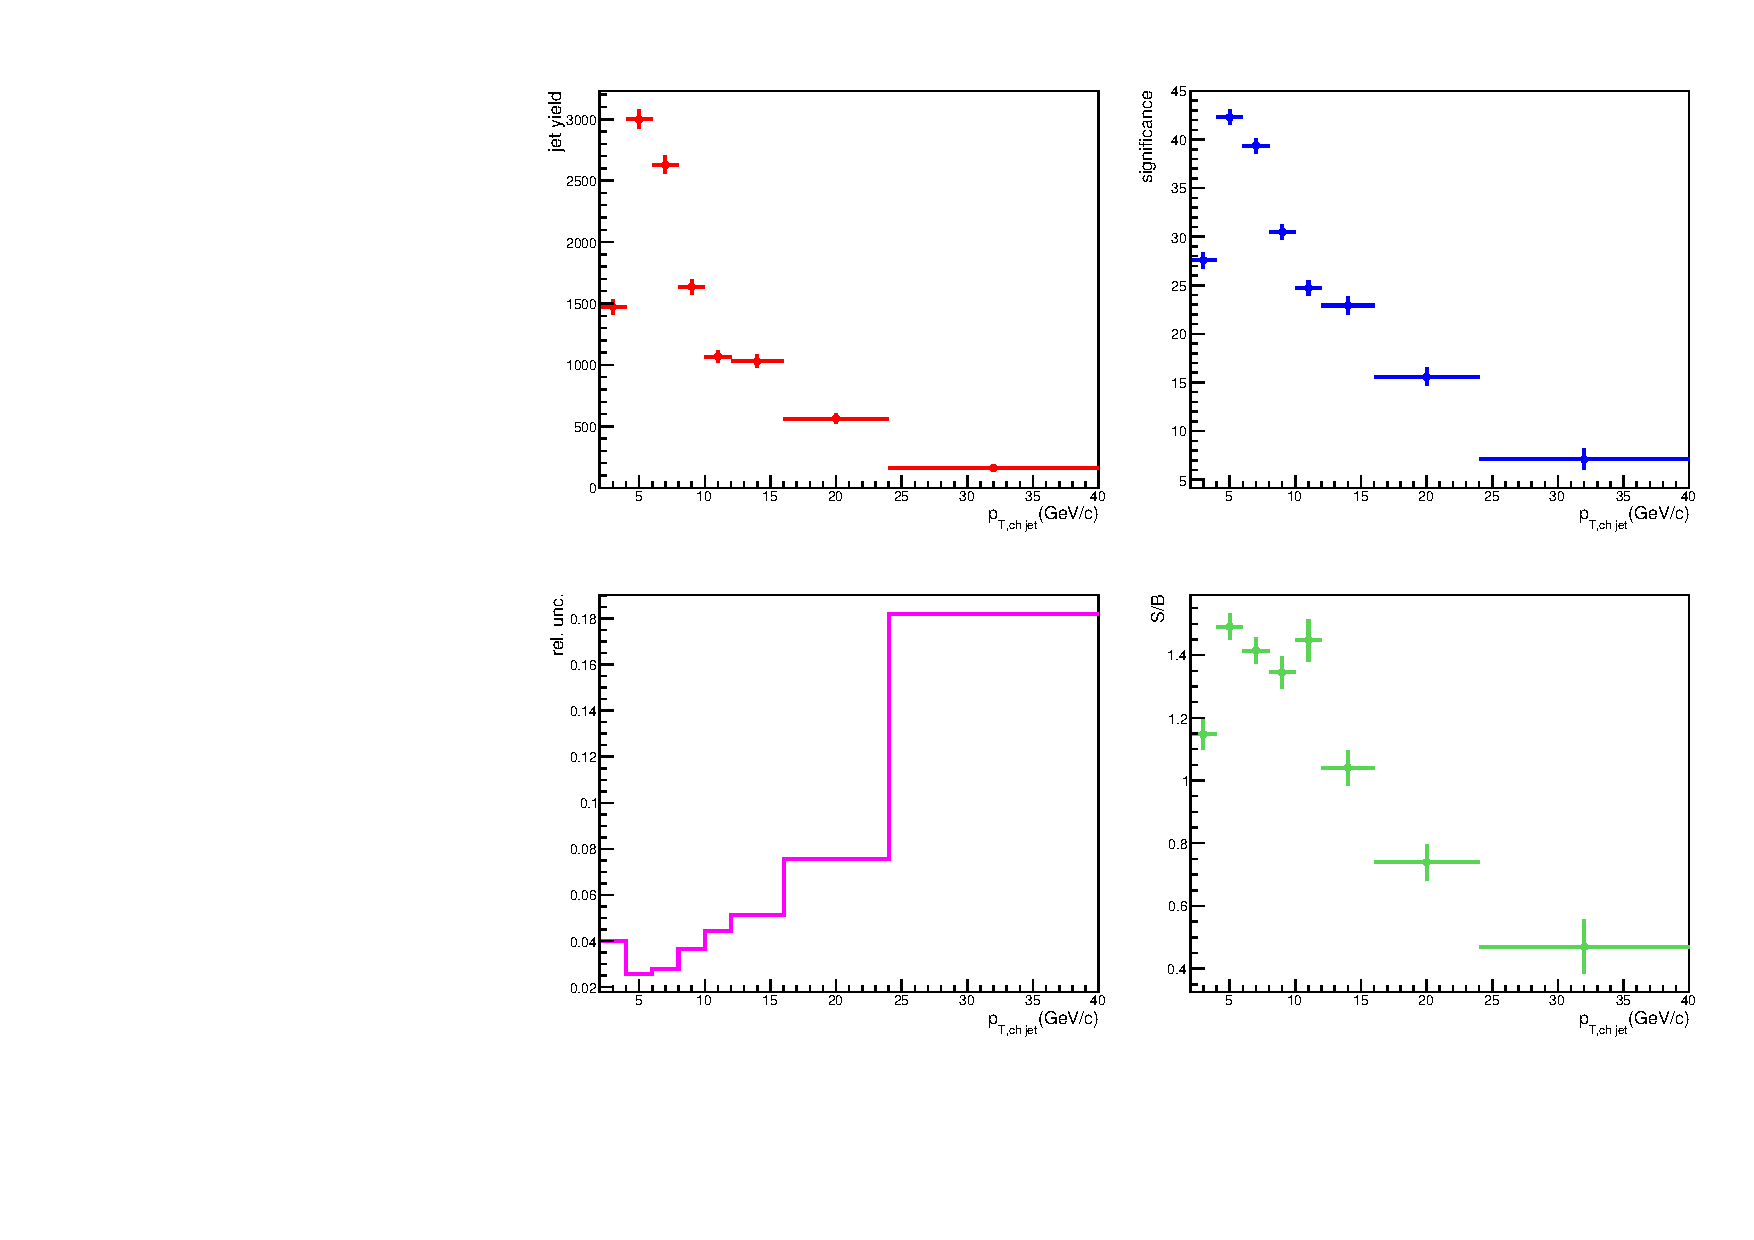
\includegraphics[width=0.7\textwidth]{pPbplots/plotsEffScale_noEff_pt3_noDetails/signalParams_FASTwoSDD}
%\caption{\Dstar-jet raw signal extraction in \pp\ collisions at $\s=5.02$~TeV for $\ptd>3$~\GeVc\ with the direct jet-\pt\ ectraction method in bins of \ptchjet.}
%\label{fig:eq_pPb_RSU_raw}
%\end{figure}
%
%The invariant mass distributions shown here are not corrected for the reconstruction efficiencies. This step is discussed in Sec.~\ref{sect:sub_DmesonRecEff}.
%The jet \pt\ bins are selected so that the significance of the D signal is above 5$\sigma$.
%The reason of the \Dstar\ signal visible in the Fig.~\ref{fig:eq_pPb_InvMass_Dstar} below \ptjet\ of 3 \GeVc\ despite the \ptd\ cut above 3 \GeVc\ is a subtraction of the jet background, as it is described in the Sec.~\ref{sBackSub}.
%%The final jet \pt\ range for the \pp\ analysis is 4 $< p_{T} < $ 40 \GeVc. 


\subsection{Side-Band Subtraction Method}
\label{sub_Bin_d_pT}

The D-meson candidates in the signal region are used to build a jet \pt\ distribution, which comprises both signal and background D-meson candidates.
Another jet \pt\ distribution is built using candidates with invariant mass that is the side-band regions: $4\sigma$ and $9\sigma$ from the peak.
The normalization is done using the information of the fit integrating the background function inside the signal area. This is done separately and independently for each \ptd\ bin.


The invariant mass distributions in bins of D-meson \pt\ are shown in Fig.~\ref{fig:eq_pPb_InvMass_Dzero_Dbins} where  the signal region is shown as the red shaded area, and the background region is depicted as the blue shaded area.
Also shown in Fig.~\ref{fig:eq_pPb_InvMass_Dzero_Dbins} are reflections for \Dzero\ in green, and their ratio over signal is shown in Fig.~\ref{fig:eq_pPb_RSU_raw_Dbins_Dzero} right.
Figure~\ref{fig:eq_pPb_RSU_raw_Dbins_Dzero} shows a summary of the raw signal extraction:
yield, relative statistical uncertainty, signal / background ratio and significance.

\begin{figure}[bth]
\centering
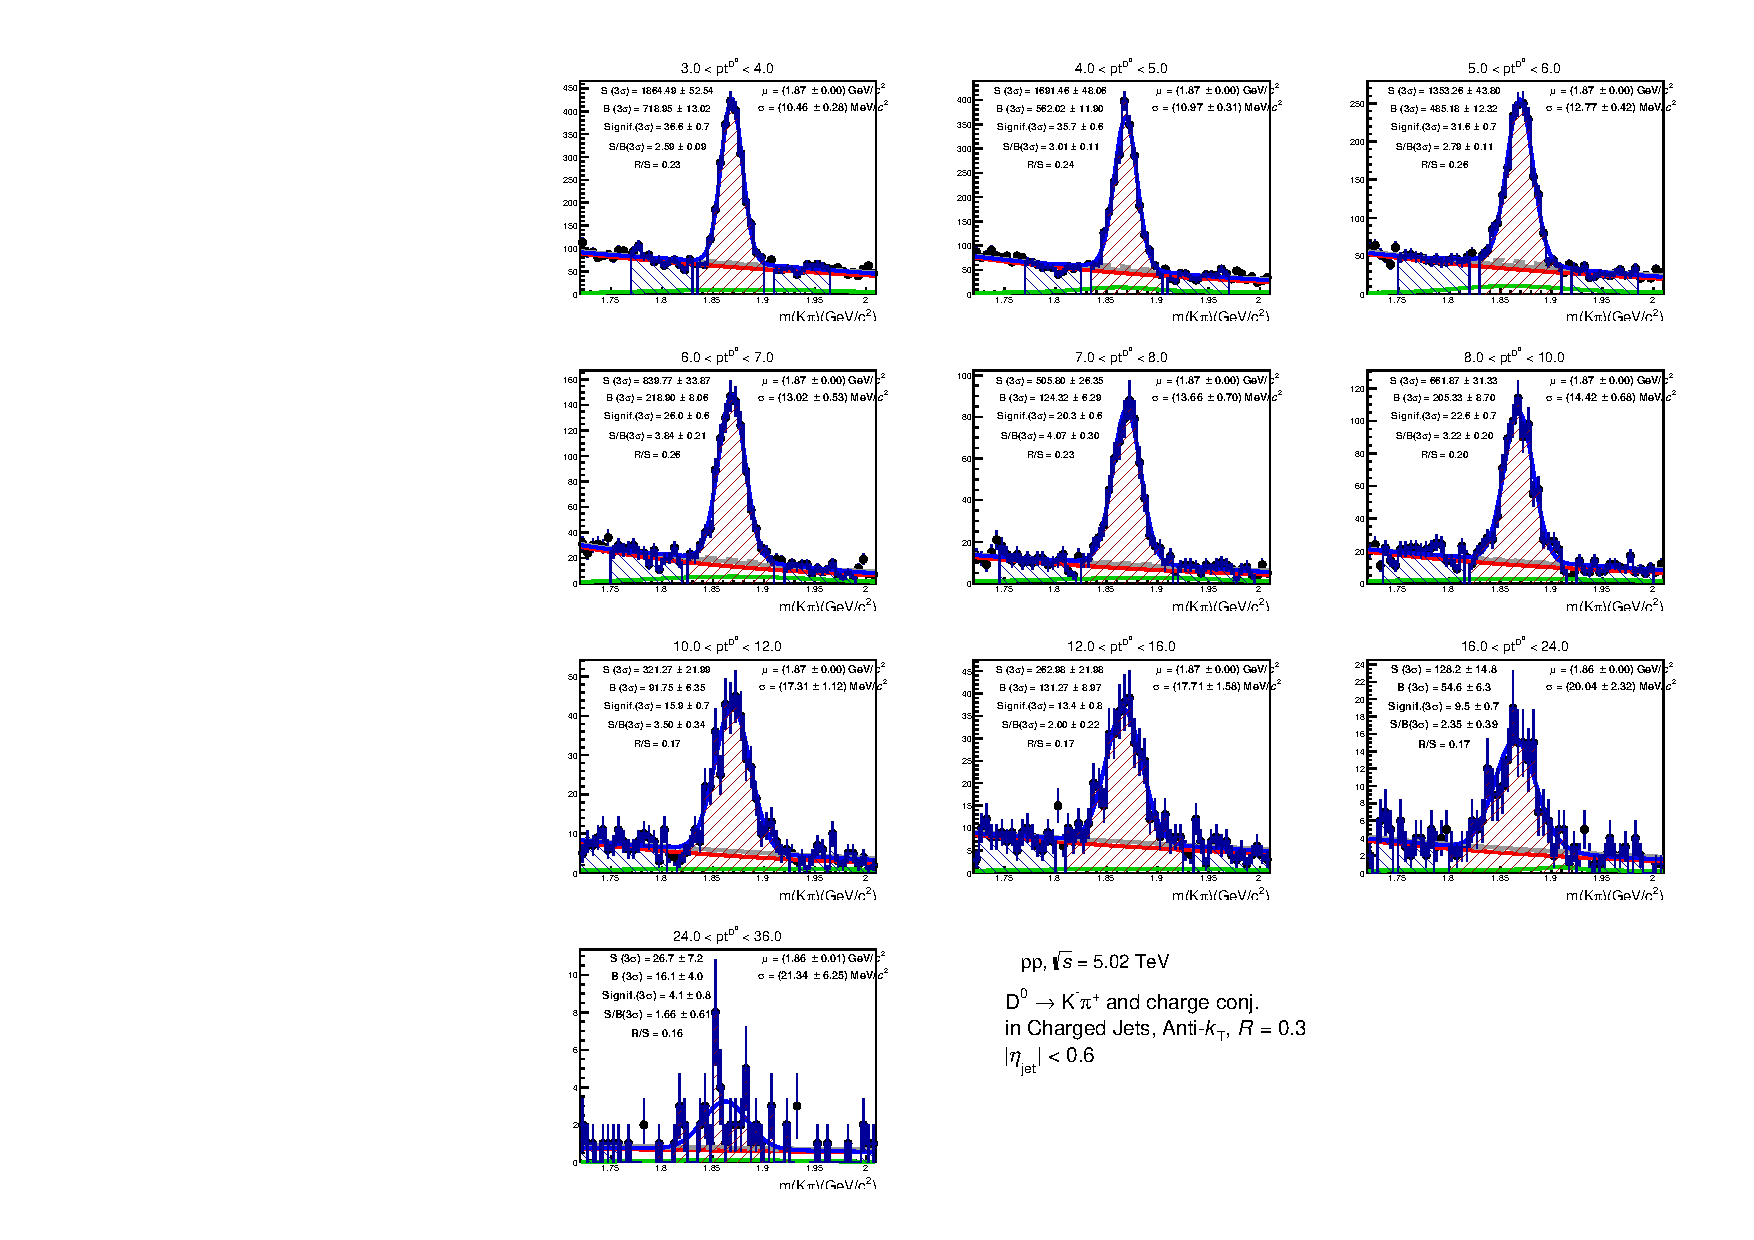
\includegraphics[width=\textwidth]{pPbcuts/invMass_pTD3}
\caption{\Dzero-jet signal extraction in bins of jet transverse momentum in \pp\ collisions at $\s=5.02$~TeV (raw yields). D mesons are required to have $\pt>3$~\GeVc. 
Reflections shown by green curve add with the combinatorial background (red curve) to give the overall background in grey.
}
\label{fig:eq_pPb_InvMass_Dzero_Dbins}
\end{figure}

\begin{figure}[bth]
\centering
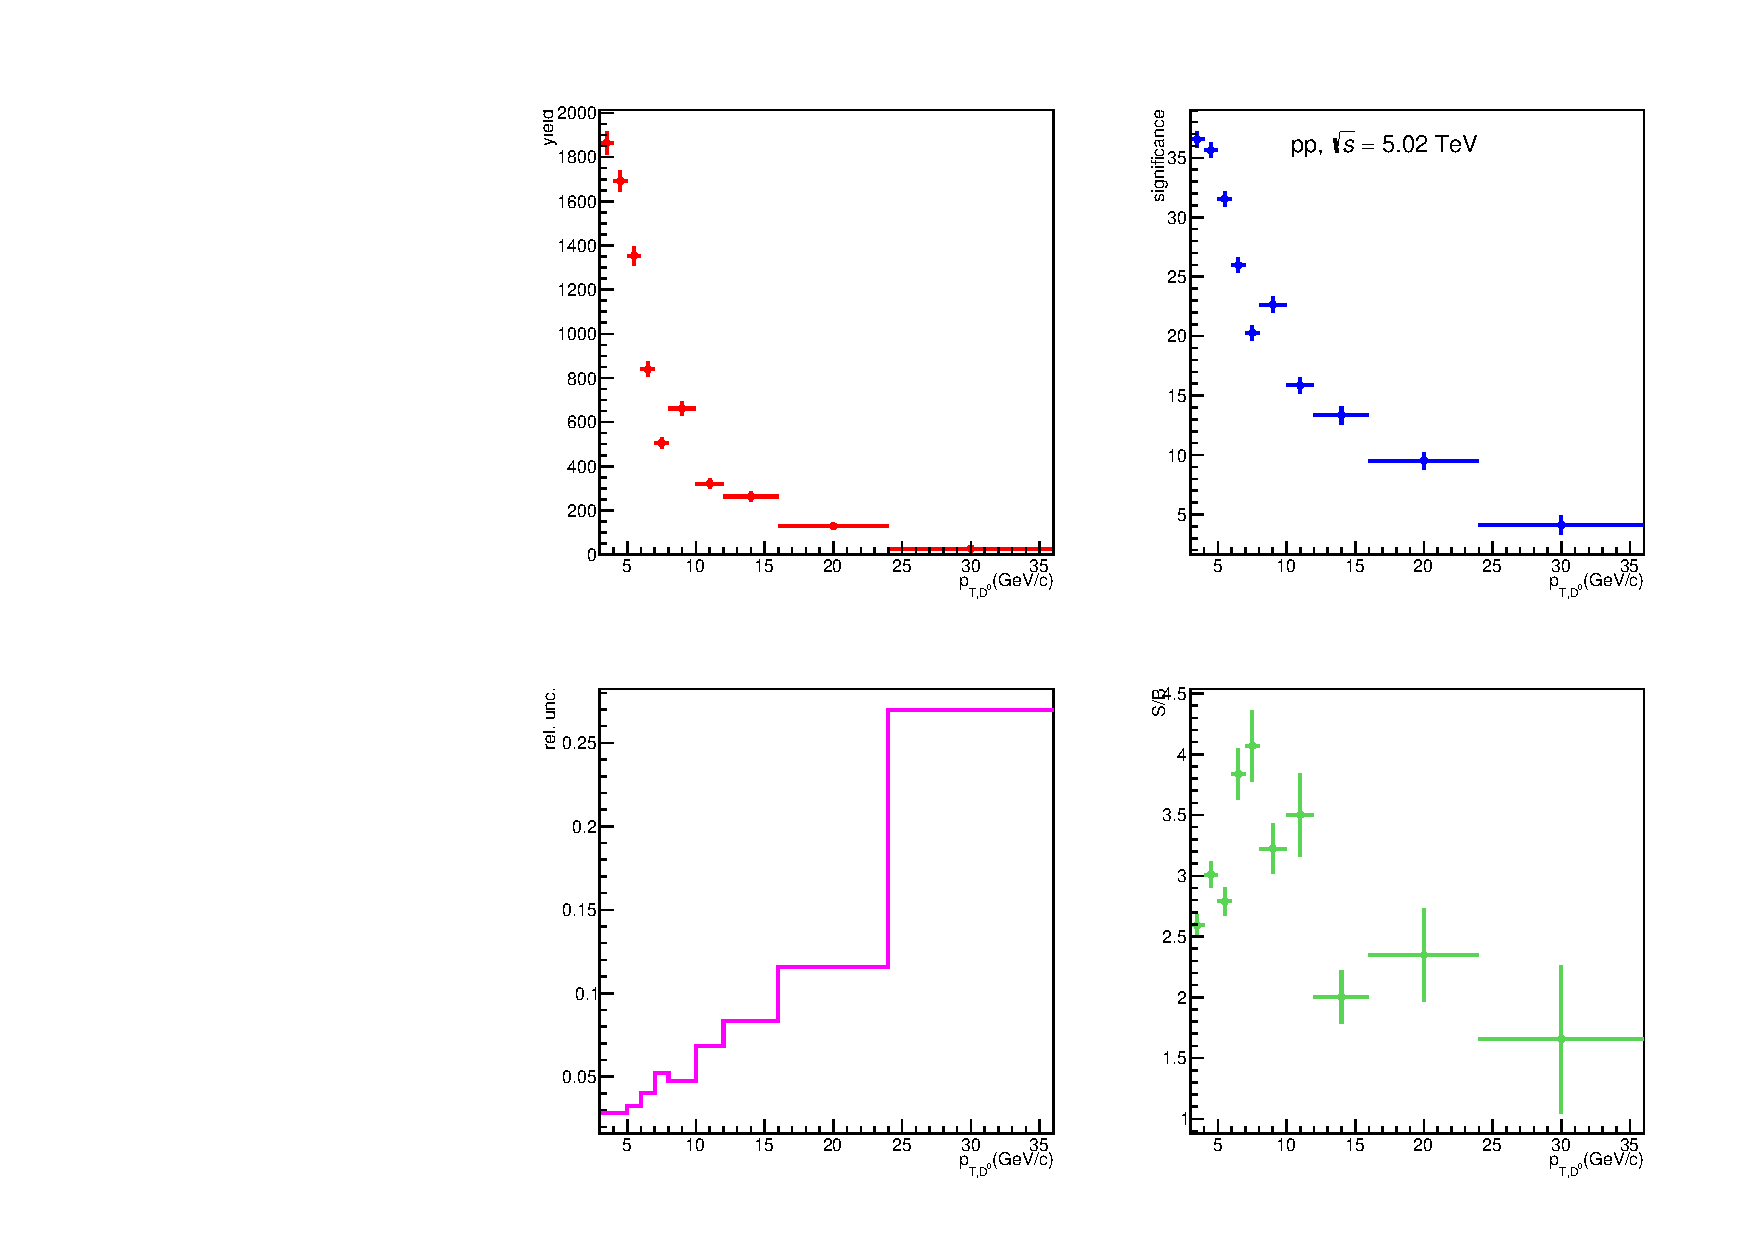
\includegraphics[width=0.63\textwidth]{pPbcuts/signalParams_pTD3}
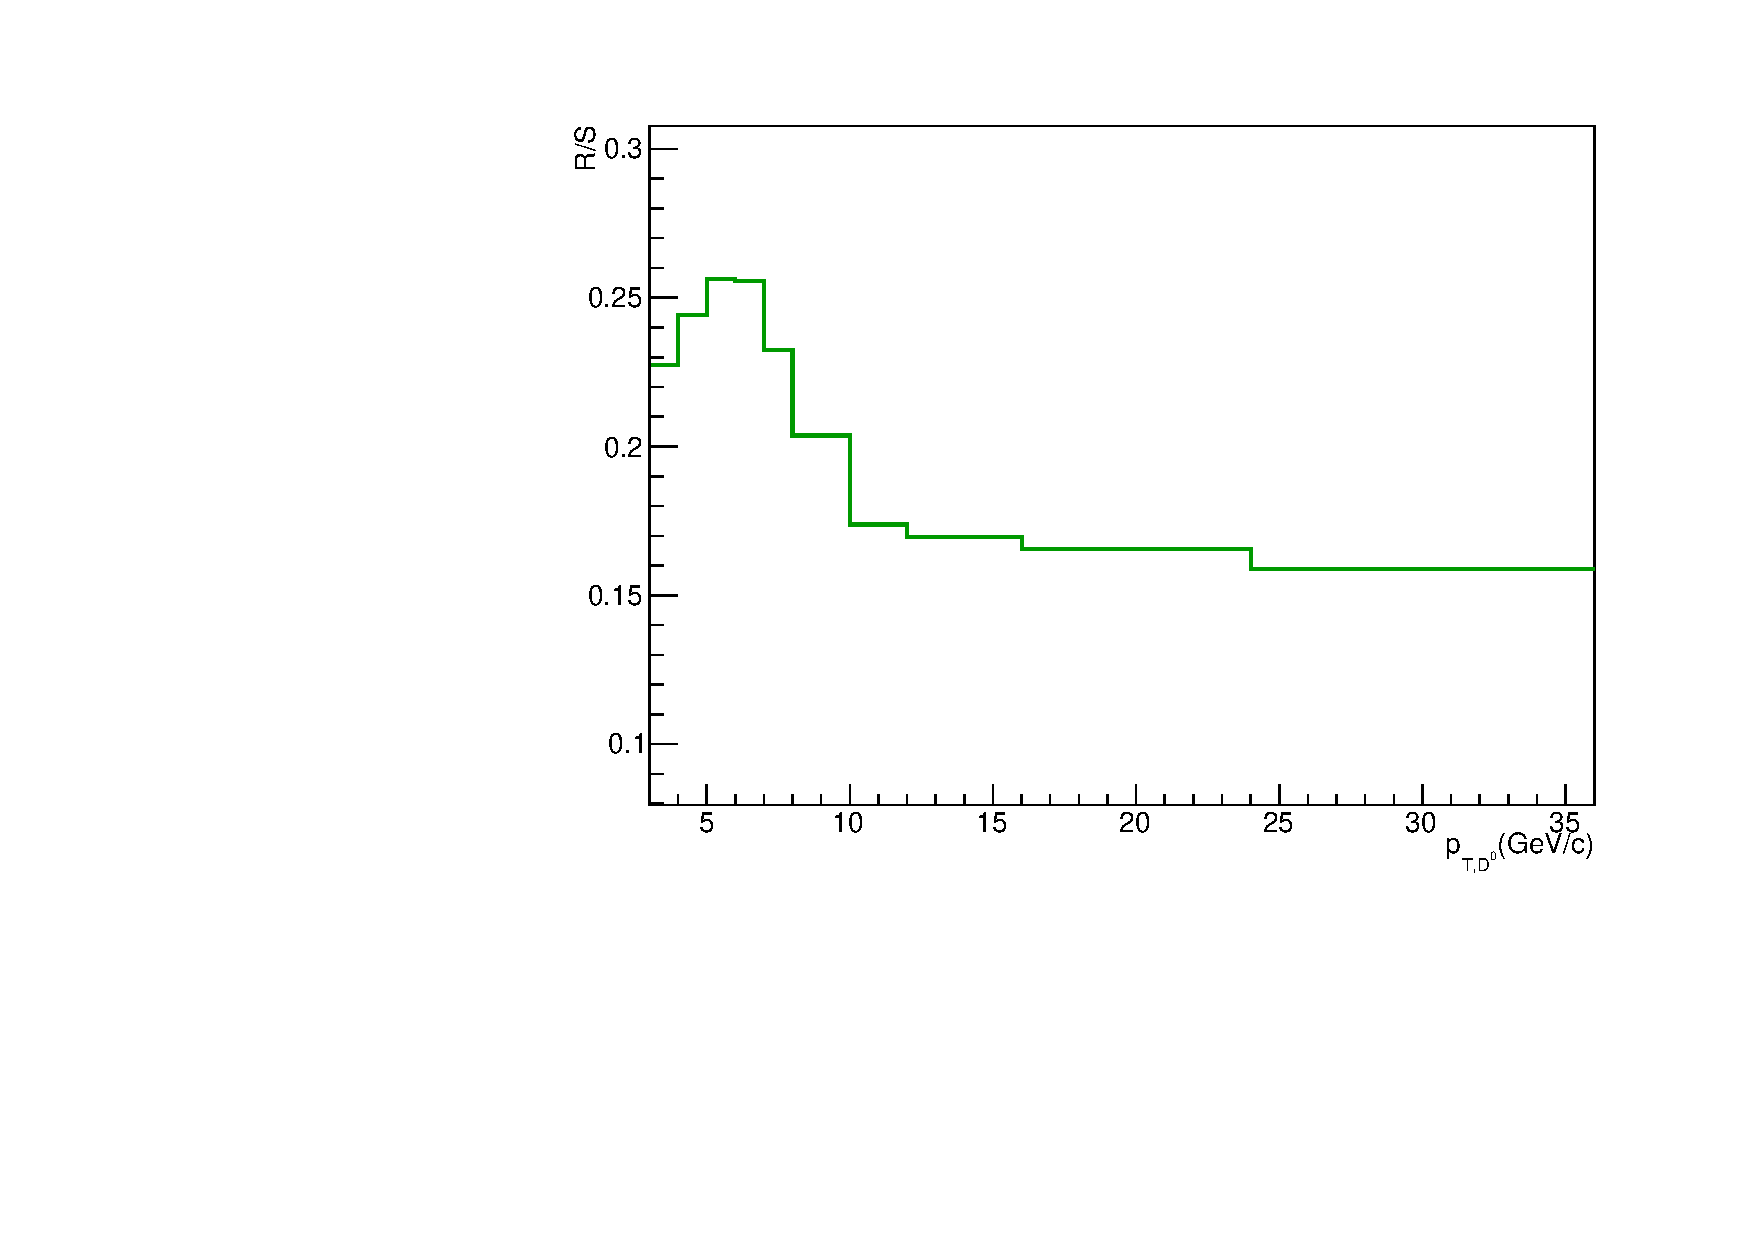
\includegraphics[width=0.35\textwidth]{pPbcuts/RefOverS_pTD3}
\caption{Left: \Dzero-jet raw signal extraction: raw yields, relative statistical uncertainties, significance and S/B ratio in \Dzero\ \pt\ bins, in \pp\ collisions at $\s=5.02$~TeV for $\ptd>3$~\GeVc\ with the Side Band method.
\\Right: \Dzero-jet raw signal extraction, reflections over signal ratio, in \pp\ collisions at $\s=5.02$~TeV for $\ptd>3$~\GeVc\ with the Side Band method.}
\label{fig:eq_pPb_RSU_raw_Dbins_Dzero}
\end{figure}

The raw jet \pt\ distributions are shown in Fig.~\ref{fig:eq_pPb_signBkgJet_Dzero_Dbins}, along with the jet \pt\ distributions for the background region. 
Then the background distributions are subtracted from the signal distributions and raw jet \pt\ distributions are obtained in each D \pt\ bin, 
as it is shown also in Fig.~\ref{fig:eq_pPb_signBkgJet_Dzero_Dbins}.
Figure~\ref{fig:eq_pPb_signBkgJet_tot} shows the sum of the jet \pt\ distributions without a correction for the D-meson-jet efficiency.

\begin{figure}[bth]
\centering
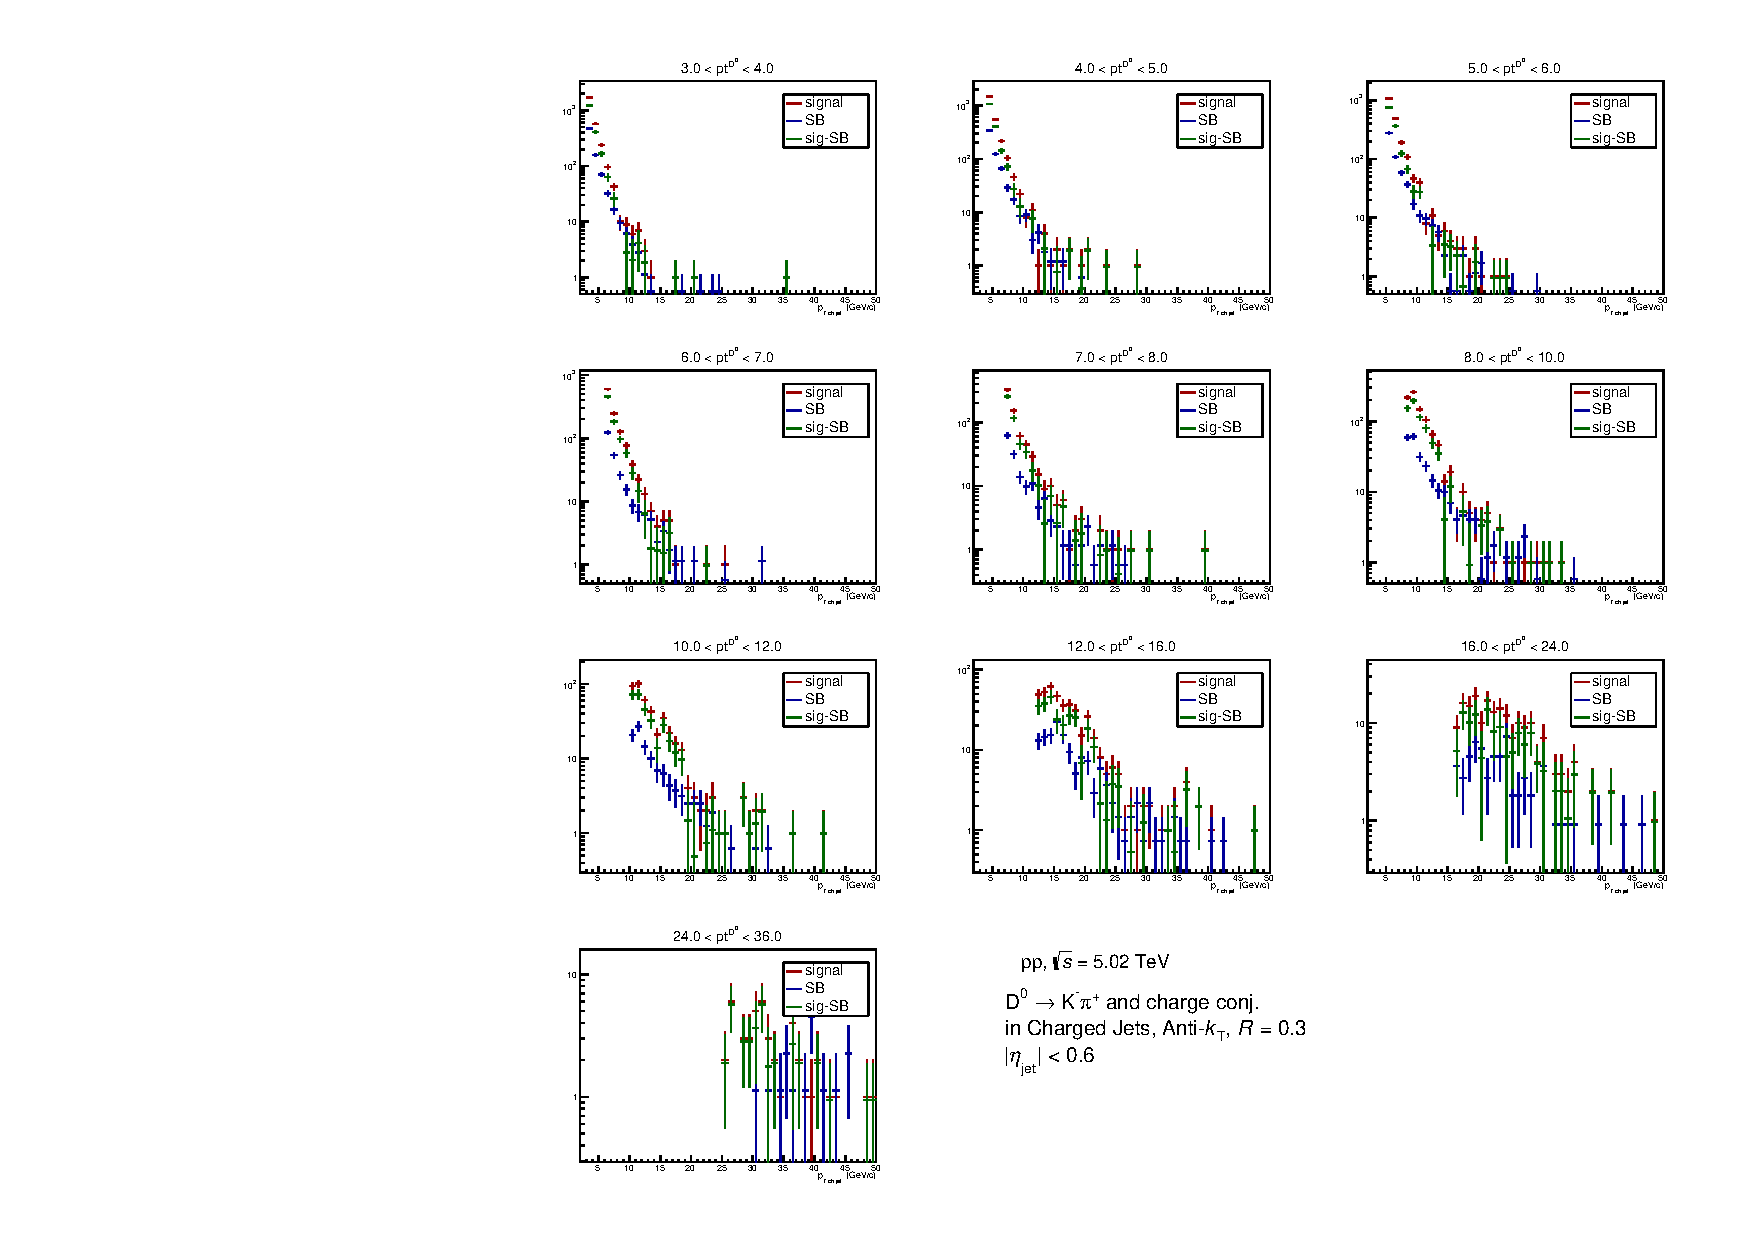
\includegraphics[width=\textwidth]{pPbcuts/jetRawSpectrum_pTD3}
\caption{Raw jet \pt\ distributions in bins of \Dzero\ transverse momentum in \pp\ collisions at $\s=5.02$~TeV.}
\label{fig:eq_pPb_signBkgJet_Dzero_Dbins}
\end{figure}

\begin{figure}[bth]
\centering
	
\includegraphics[width=0.3\textwidth]{missing}%pPbcuts/jetPtSpectrum_SB_pTD3_noeff}
	
\includegraphics[width=0.3\textwidth]{missing}%pPbcuts/jetPtSpectrum_SB_Rebin_pTD3_noeff}
\caption{Total raw jet \pt\ distributions (left) in \pp\ collisions at $\s=5.02$~TeV, obtained summing together all D \pt\ bins without an efficiency correction. The same after rebbining (right).}
\label{fig:eq_pPb_signBkgJet_tot}
\end{figure}

In order to obtain the final jet \pt\ spectrum, the distributions in each D \pt\ bin need to be corrected for the D efficiency and finally summed up.
The corrections will be discussed in Section~\ref{sect:sub_DmesonRecEff}. 
%\newpage
%\newpage


%%%%%%%%%%%%%%%%%%%%%%%%%%%%%%%%%%%%%%%%%%%%%%%%%%%%%%%%%%%%%%%%%%%%%%
%%%%%%%%%%%%%%%%%%%%%%%%%%%%%%%%%%%%%%%%%%%%%%%%%%%%%%%%%%%%%%%%%%%%%%
%%%%%%%%%%%%%%%%%%%%%%%%%%%%           EFFICIENCY            %%%%%%%%%%%%%%%%%%%%%%%%%%%%
%%%%%%%%%%%%%%%%%%%%%%%%%%%%%%%%%%%%%%%%%%%%%%%%%%%%%%%%%%%%%%%%%%%%%%
%%%%%%%%%%%%%%%%%%%%%%%%%%%%%%%%%%%%%%%%%%%%%%%%%%%%%%%%%%%%%%%%%%%%%%

\section{Efficiency Correction Procedure}

\subsection{Reconstruction Efficiency}
\label{sect:sub_DmesonRecEff}
The efficiency and acceptance (${\rm Acc} \times \epsilon$) were calculated using Monte Carlo PYTHIA6+GEANT3 simulations anchored to the data.

The efficiency is taken as the ratio of the \ptd\ spectra of the D-tagged generator-level jets for which a matched
D-tagged detector-level jet was found over all the generated D-tagged jets.
For the detector-level jets, the D meson is required to be within the standard fiducial rapidity cuts.
Jets are further requested to have $|\eta_{\rm jet}| < 0.9 - R$, both at generator and detector levels.

\begin{figure}[bth]
\centering
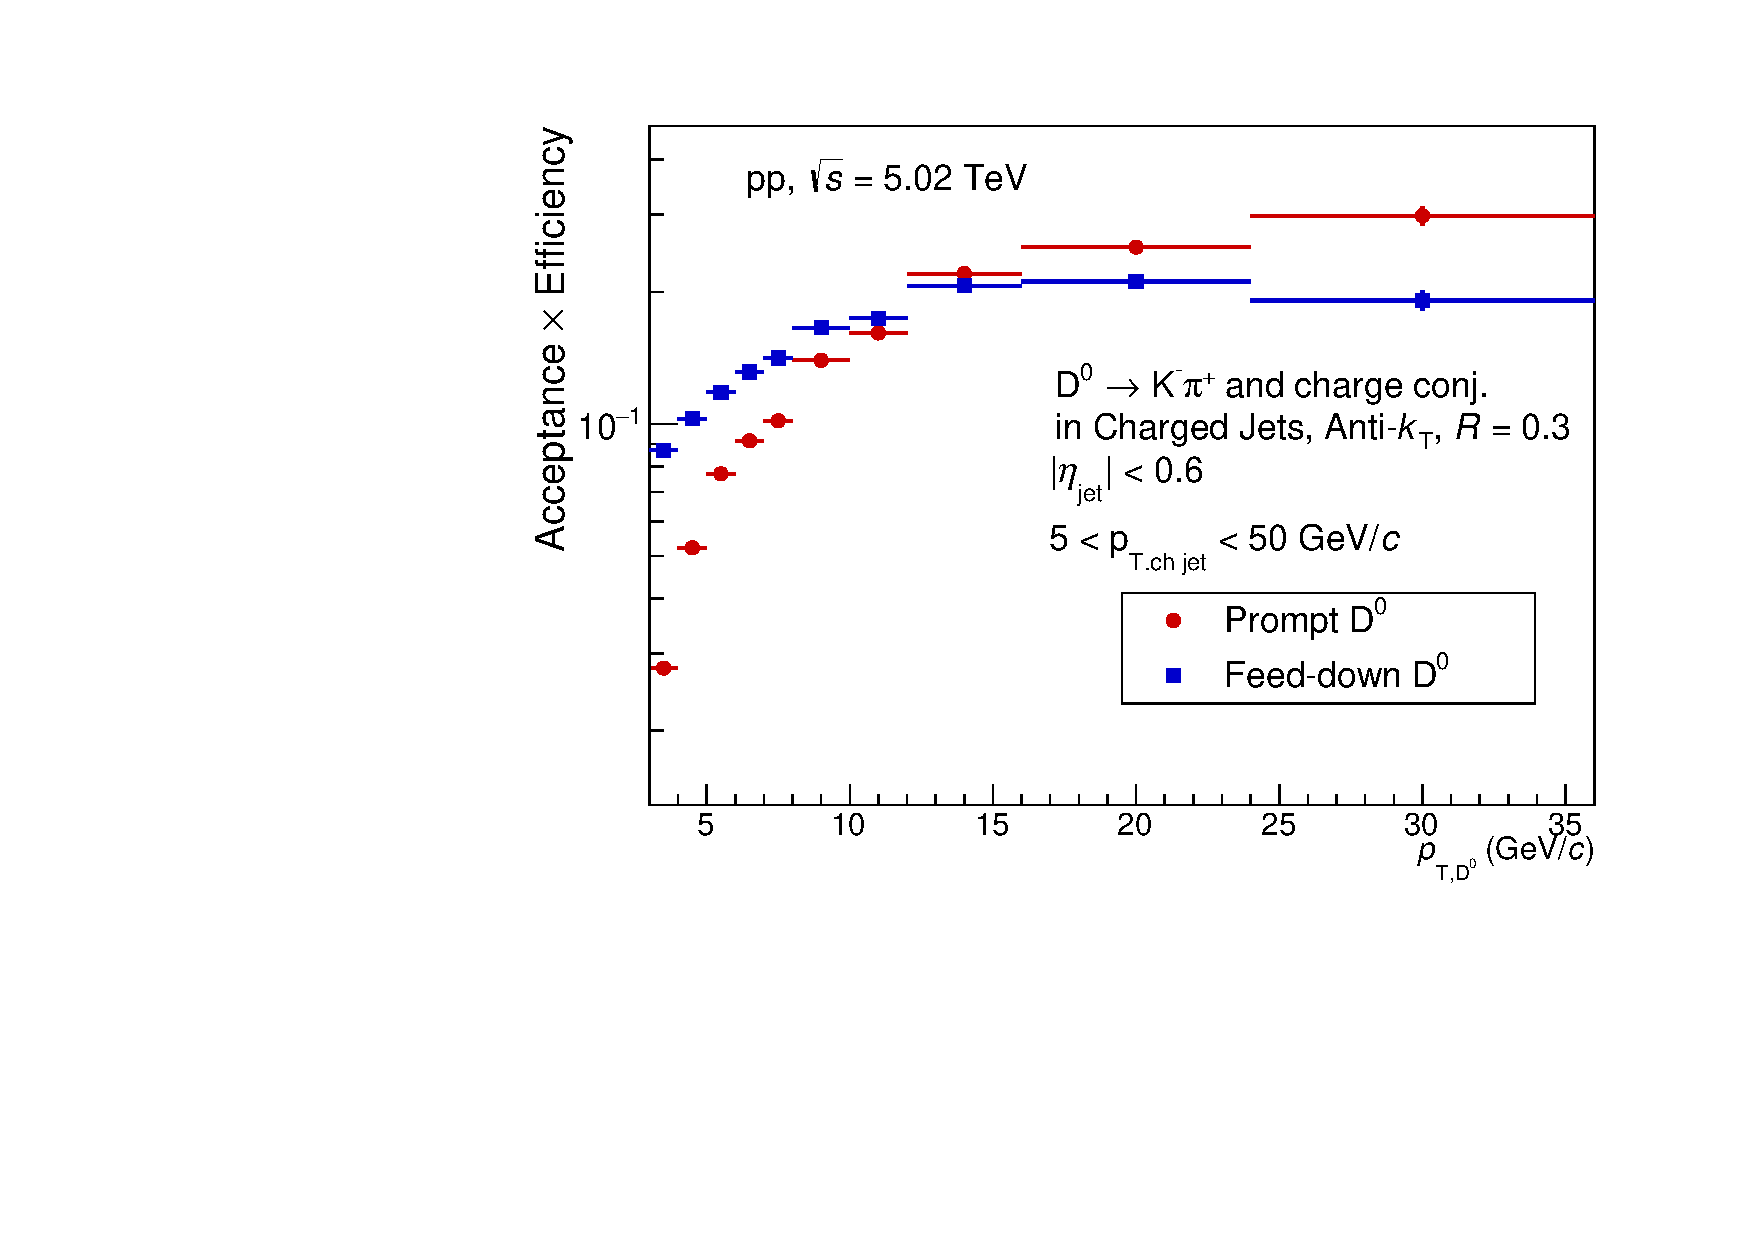
\includegraphics[width=0.6\textwidth]{pPbcuts/DjetEff_Sim_log}
\caption{\Dzero-meson-jet reconstruction efficiencies in \pp\ collisions at $\s=5.02$~TeV, for prompt D mesons in red and non-prompt in blue.}
\label{fig:eq_pp_DrecEff}
\end{figure}

Figure~\ref{fig:eq_pp_DrecEff} shows the \Dzero\-jet reconstruction efficiencies as a function of \ptd\, 
for prompt and non-prompt D-mesons. Efficiency depends strongly on \ptd\ because of the topological cuts that are relaxed at higher momenta where the combinatorial background is smaller. 
The efficiency is with a cut on \ptchjet\ of $5 < \ptchjet < 50$ \GeVc\ (range of the final \Dzero-tagged jet \pt\ spectrum) at the generator level, applied for both denominator and nominator in the efficiency calculation.

%However a very weak or no dependence on \ptchjet\ is observed for $5<\ptchjet<30$~\GeVc. From the ratios of the efficiencies in \ptchjet\ bins over the entire range, shown in Fig.~\ref{fig:eq_pp_DrecEff_ptd_ptjet} one can appreciate a hint of a small deviation, on the order of 10-20\%, for low momentum \Dzero\ (\ptd~$<5$~\GeVc) in high momentum jets. However this deviation is not statistically significant, and affects a very small fraction of the D-meson candidates.

\subsection{Efficiency-Corrected Yields}

As discussed in the previous section, the D-meson reconstruction efficiency shows a strong dependence on \ptd\ (but has very weak or no dependence on \ptjet).
Therefore, in order to reduce the dependence on the Monte Carlo simulation for what concerns jet fragmentation and momentum spectral shape,
the efficiency should be applied as a function of the D-meson momentum. In fact, each bin of \ptjet\ has contributions from D mesons with very different \ptd, which have different efficiencies.

%\subsubsection{Direct Jet-$p_T$ Extraction Method}
%
%The efficiency-rescaling procedure of the invariant mass distribution $M(\ptjet,\ptd)$ was implemented according to the following formula:
%\begin{equation}
%M(\ptjet) = \displaystyle\sum_{\ptd}\frac{M(\ptjet,\ptd)}{({\rm Acc} \times \epsilon)_{\ptd}}.
%\end{equation}
%
%Figure~\ref{fig:eq_pPb_Directjet_corrInv_Dstar} shows the \Dstar\ invariant mass distributions for different ranges of \ptchjet, after the efficiency reweighing procedure.
%%Figures~\ref{fig:eq_pPb_Directjet_corrInv_Dstar} and \ref{fig:eq_pPb_Directjet_corrInv_Dzero} show the \Dstar\ and \Dzero\ invariant mass distributions 
%for different ranges of \ptchjet, after the efficiency reweighing procedure.
%%This process can increase the relative statistical uncertainty due to the large weight assigned to low-\pt\ D mesons (low reconstruction efficiency). 
%
%%Dstar
%\begin{figure}[bth]
%\centering
%\includegraphics[width=0.9\textwidth]{pPbplots/plotsEffScale_pt3_noDetails/invMass_FASTwoSDD}
%\caption{\Dstar\ signal extraction in bins of jet transverse momentum in \pp\ collisions at $\s=5.02$~TeV. D mesons are required to have $\ptd>3$~\GeVc.
%Each candidate is weighted by the inverse of the reconstruction efficiency, which depends on its \ptd.}
%\label{fig:eq_pPb_Directjet_corrInv_Dstar}
%\end{figure}
%
%%Dzero
%%\begin{figure}[bth]
%%\centering
%%\includegraphics[width=0.9\textwidth]{pPbplotsD0/}
%%\caption{\Dzero\ signal extraction in bins of jet transverse momentum in \pp\ collisions at $\s=5.02$~TeV. D mesons are required to have $\ptd>3$~\GeVc.
%%Each candidate is weighted by the inverse of the reconstruction efficiency, which depends on its \ptd.}
%%\label{fig:eq_pPb_Directjet_corrInv_Dzero}
%%\end{figure}
%%
%
%%Figure~\ref{fig:eq_pPb_RSU_raw_corrDrec} shows the yield and relative statistical uncertainties of the reconstructed D-tagged jets with the efficiency weighting with the invariant mass fit method. A comparison with ~\ref{fig:eq_pPb_RSU_raw} shows  that the relative statistical uncertainties are increased as a result of the efficiency weighting.

\subsubsection{Side-Band Subtraction Method}
In the side-band method the efficiency correction is applied by rescaling the D-jet background subtracted \pt\ spectra in Fig.~\ref{fig:eq_pPb_signBkgJet_Dzero_Dbins}
by 1/(${\rm Acc} \times \epsilon$) in each D-meson \pt\ bin shown in Fig.~\ref{fig:eq_pp_DrecEff}, where $\epsilon$ is the prompt D-jet reconstruction efficiency.
The distributions are then summed up to obtain the corrected jet \pt\ spectra for D-jets. 
The efficiency corrected jet $p_{T}$ spectra are shown in Fig.~\ref{fig:eq_pPb_Directjet_corrSum} (left), and after rebining in Fig.~\ref{fig:eq_pPb_Directjet_corrSum} (right).

\begin{figure}[bth]
\centering
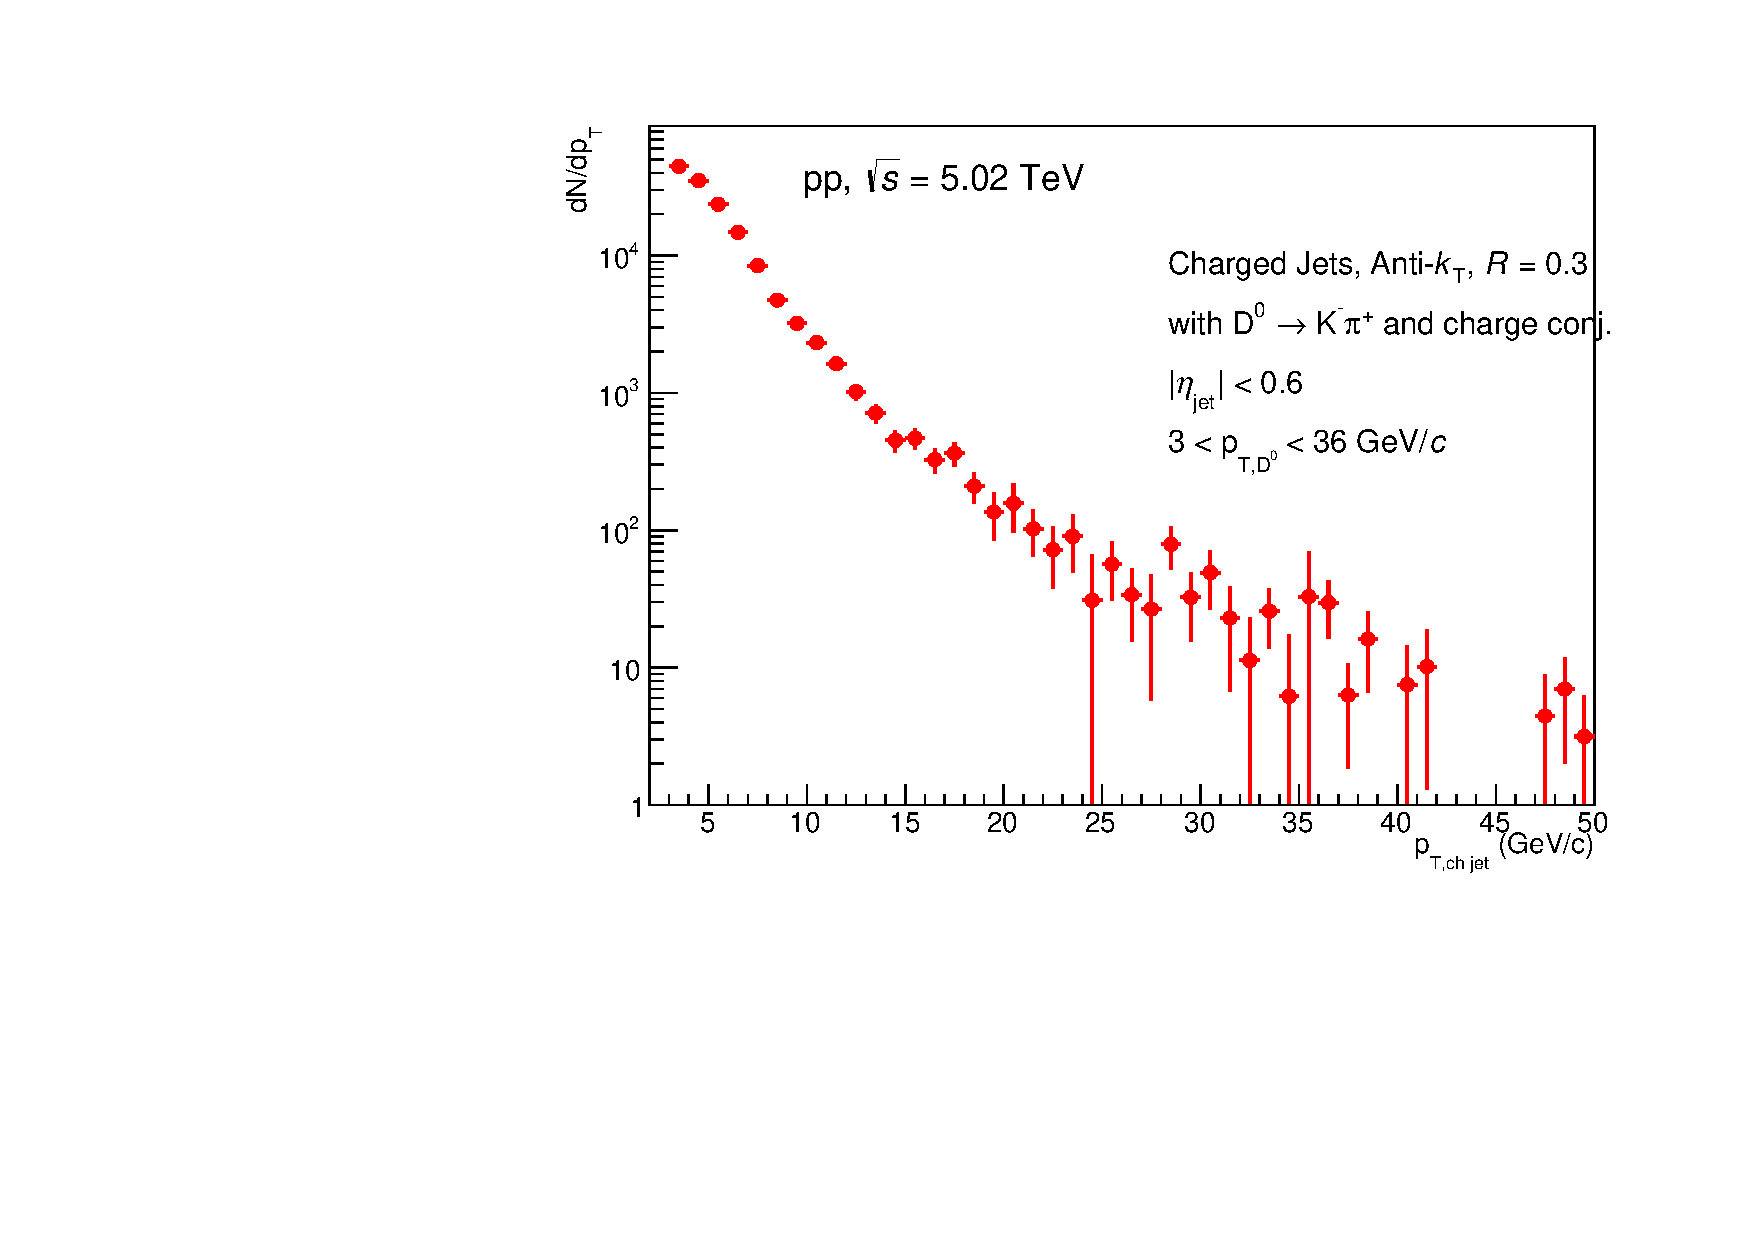
\includegraphics[width=0.45\textwidth]{pPbcuts/jetPtSpectrum_SB_pTD3}
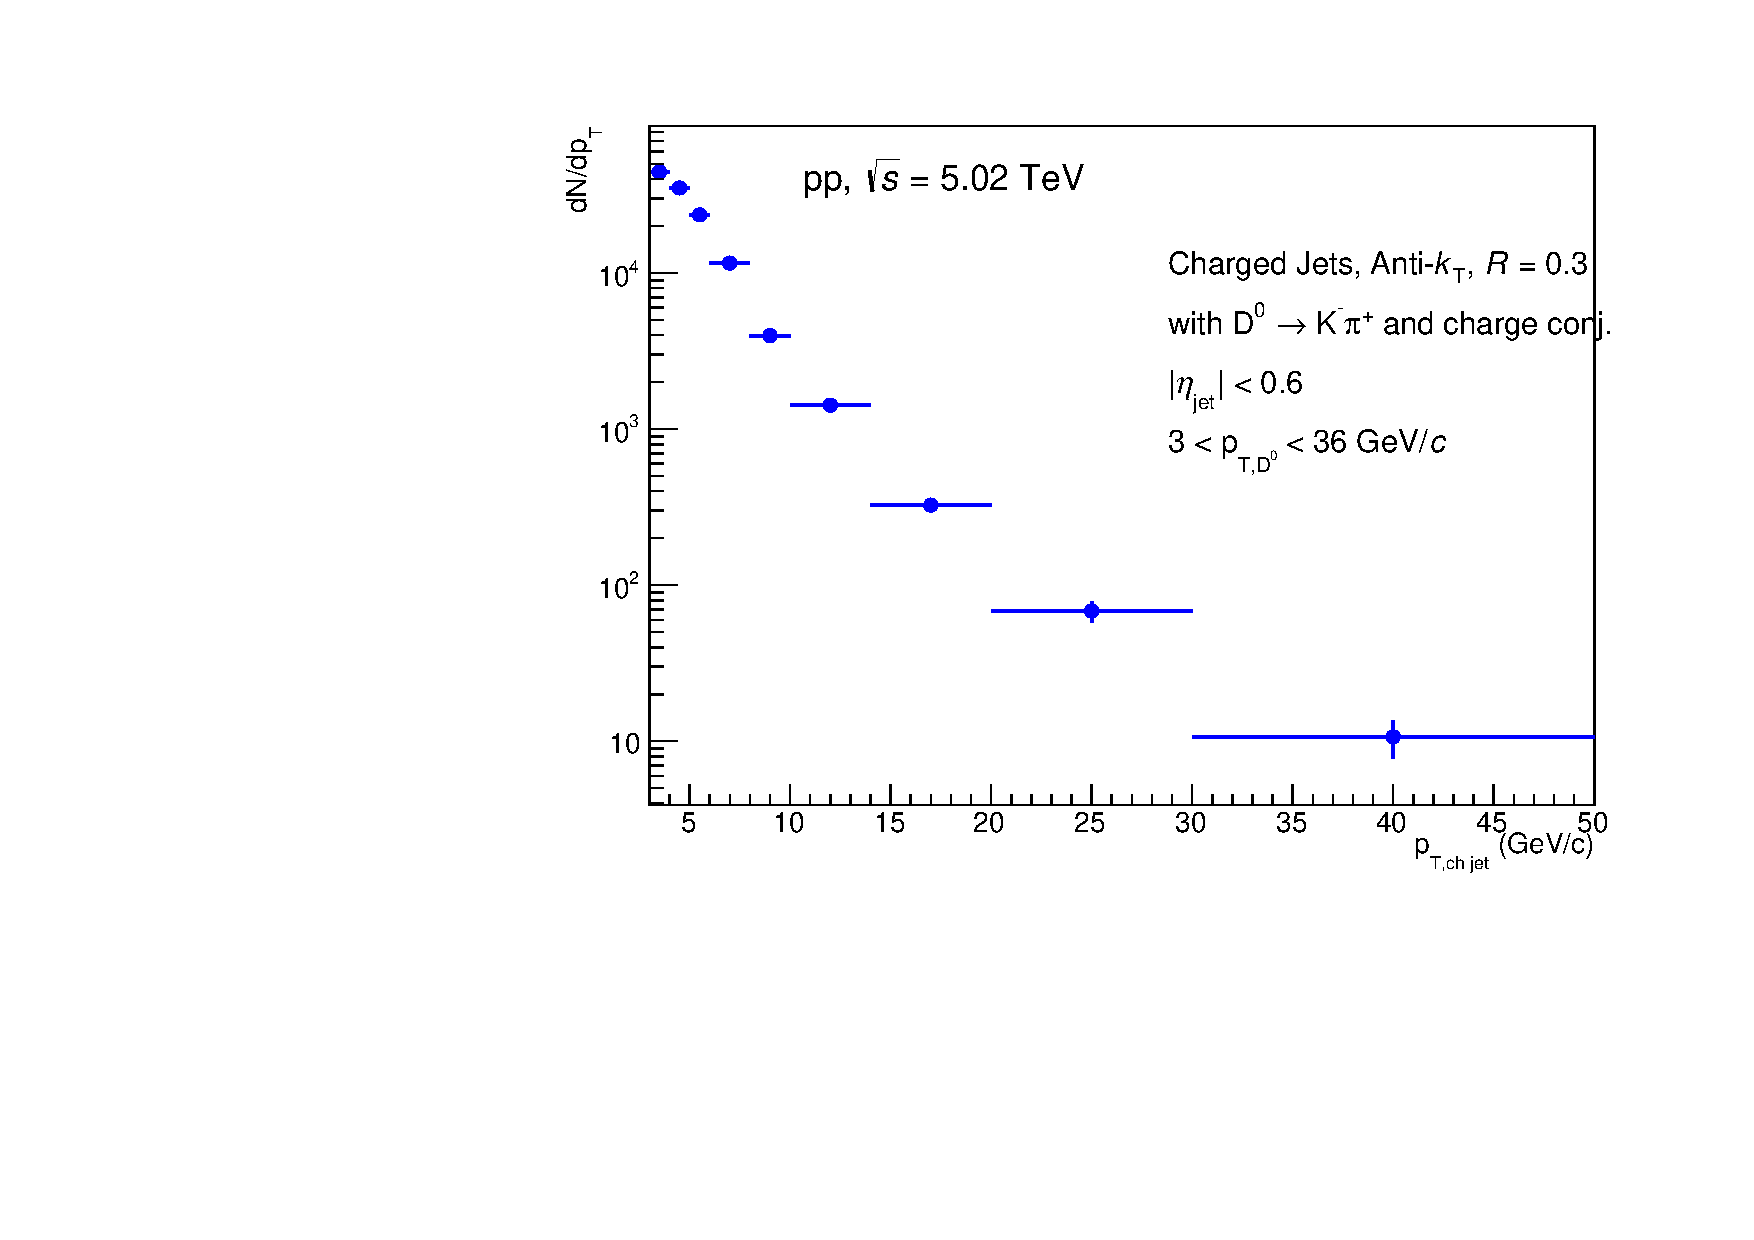
\includegraphics[width=0.45\textwidth]{pPbcuts/jetPtSpectrum_SB_Rebin_pTD3}
\caption{Efficiency corrected D-jet yield obtained for the Side-Band subtraction method in \pp\ collisions at $\s=5.02$~TeV. D mesons are required to have 3 $< \ptd<$ 36~\GeVc. Right: after rebinning.}
\label{fig:eq_pPb_Directjet_corrSum}
\end{figure}


Figure~\ref{fig:JetPt_pPb_SBUnc_Dzero} shows the relative statistical uncertainties for the Side-Band subtraction method with $\ptd>3$~\GeVc. %The measurement extents the \ptchjet\ reach to 50 \GeVc\, while the previous \pp\ measurement extended up to \GeVc\ with significantly higher statistical uncertainties.

\begin{figure}[bth]
\centering
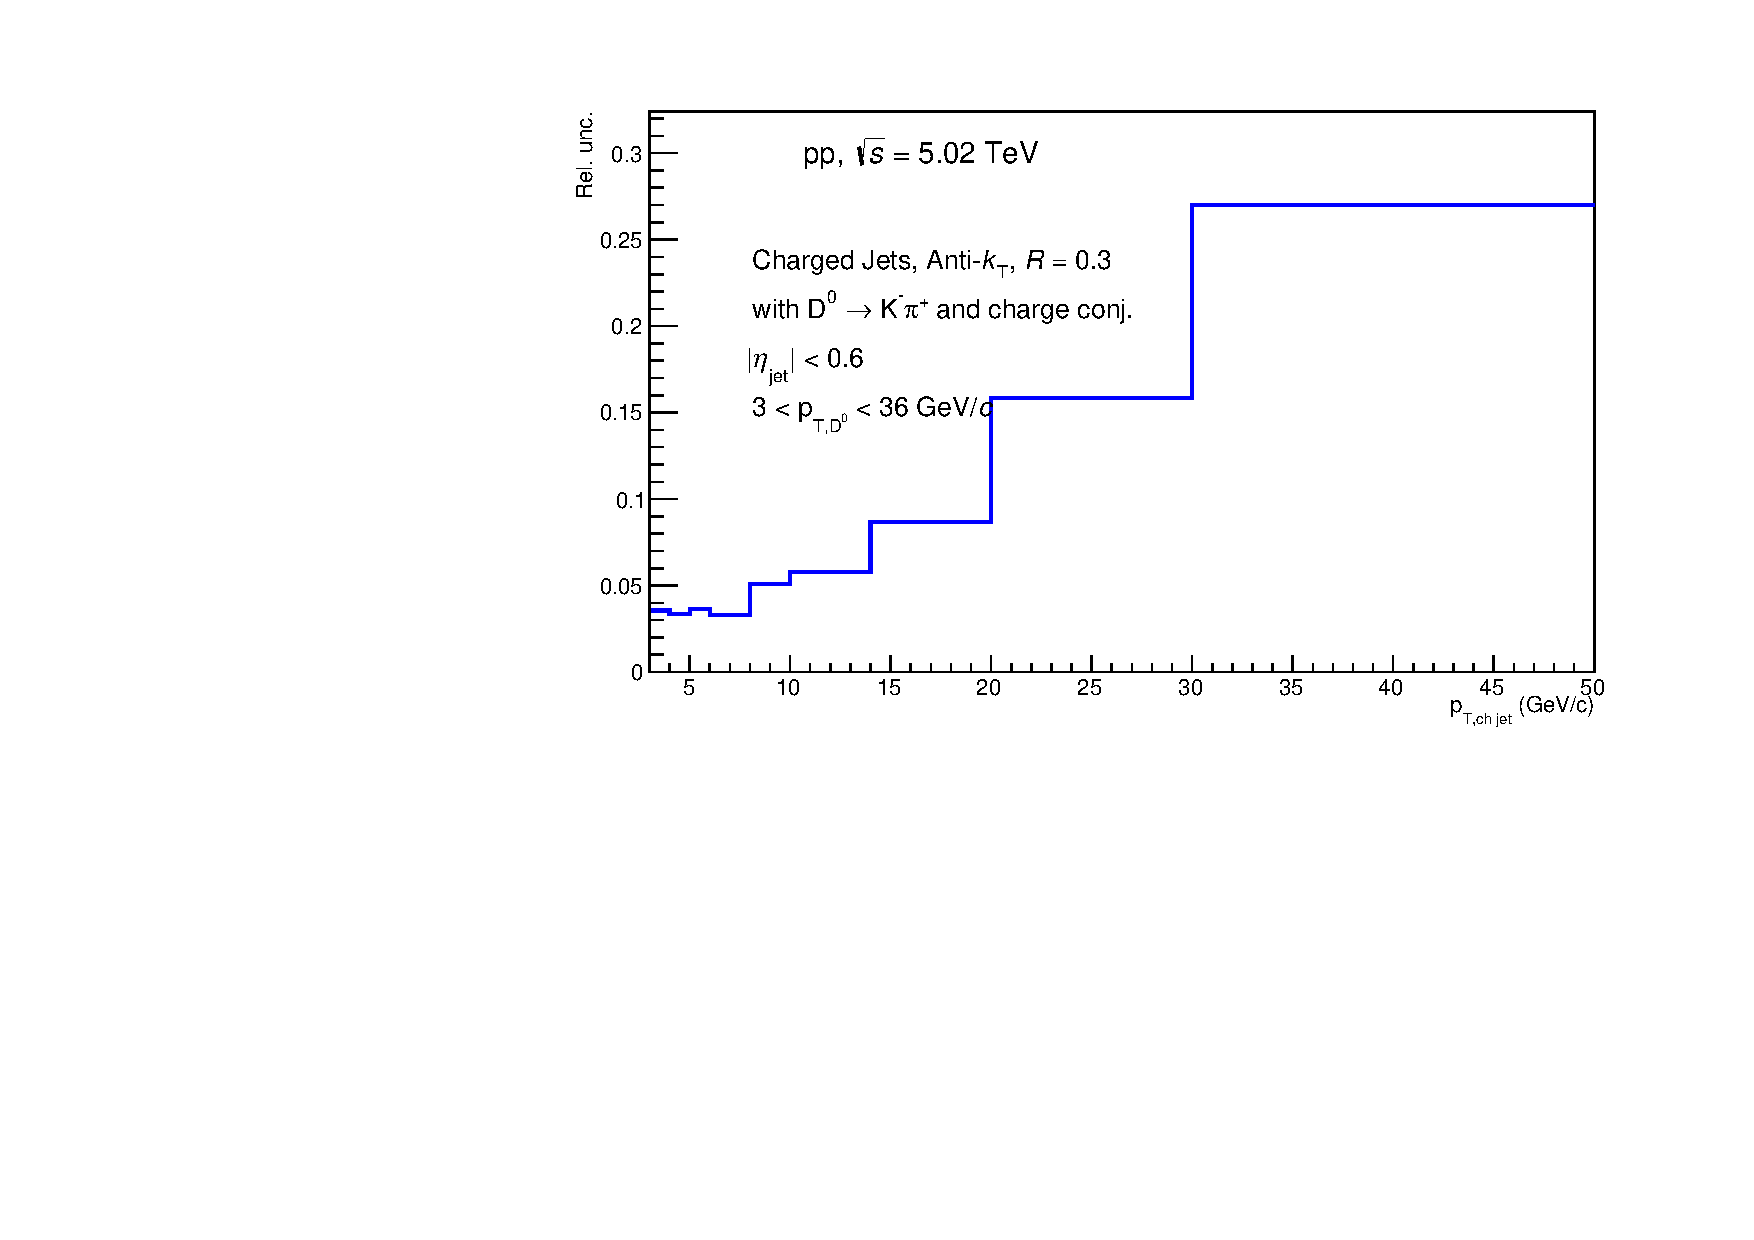
\includegraphics[width=0.6\textwidth]{pPbcuts/jetPtSpectrumUnc_SB_Rebin_pTD3}
\caption{Statistical uncertainties obtained using the side band method for \Dzero-jets in \pp\ at $\s=5.02$~TeV, with $\ptd>3$~\GeVc\ . Reconstruction efficiency correction is applied.}
\label{fig:JetPt_pPb_SBUnc_Dzero}
\end{figure}


%\subsection{Method Comparison (Efficiency-Corrected Yields)}
%
%Figure~\ref{fig:JetPt_pPb_corrDrec_Dstar} shows a comparison of the efficiency-corrected yields obtained using the direct jet-\pt\ extraction method 
%and the side band subtraction method for \Dstar-jets with $\ptd>2$~\GeVc\ and $\ptd>3$~\GeVc. 
%%Figure~\ref{fig:JetPt_pPb_corrDrec_Dstar} and \ref{fig:JetPt_pPb_corrDrec_Dzero} show a comparison of the efficiency-corrected yields obtained using the direct jet-\pt\ extraction method and the side band subtraction method for \Dstar-jets and \Dzero-jets respectively with $\ptd>2$~\GeVc\ and $\ptd>3$~\GeVc. 
%As mentioned before, the direct jet-\pt\ extraction method is sensitive to weighing with low efficiency for low $p_{T}$ D mesons. 
%Therefore, discrepancies for higher \ptjet\ ranges between two methods are visible with $\ptd>2$~\GeVc\ cut. 
%With $\ptd>3$~\GeVc\ cut the two methods agree very well with each other within the statistical uncertainties.
%$\ptd>3$~\GeVc\ cut reduces also uncertainties on the jet spectra for higher \ptjet. 
%
%
%%Figure~\ref{fig:JetPt_pPb_SBUnc} shows relative statistical uncertanties for the Side-Band subtraction method with $\ptd>2$~\GeVc\ and $\ptd>3$~\GeVc; $\ptd>3$~\GeVc\ cut reduces also uncertainties on the jet spectra for higher \ptjet. 
%
%\begin{figure}[bth]
%\centering
%\begin{subfigure}[b]{0.45\textwidth}
%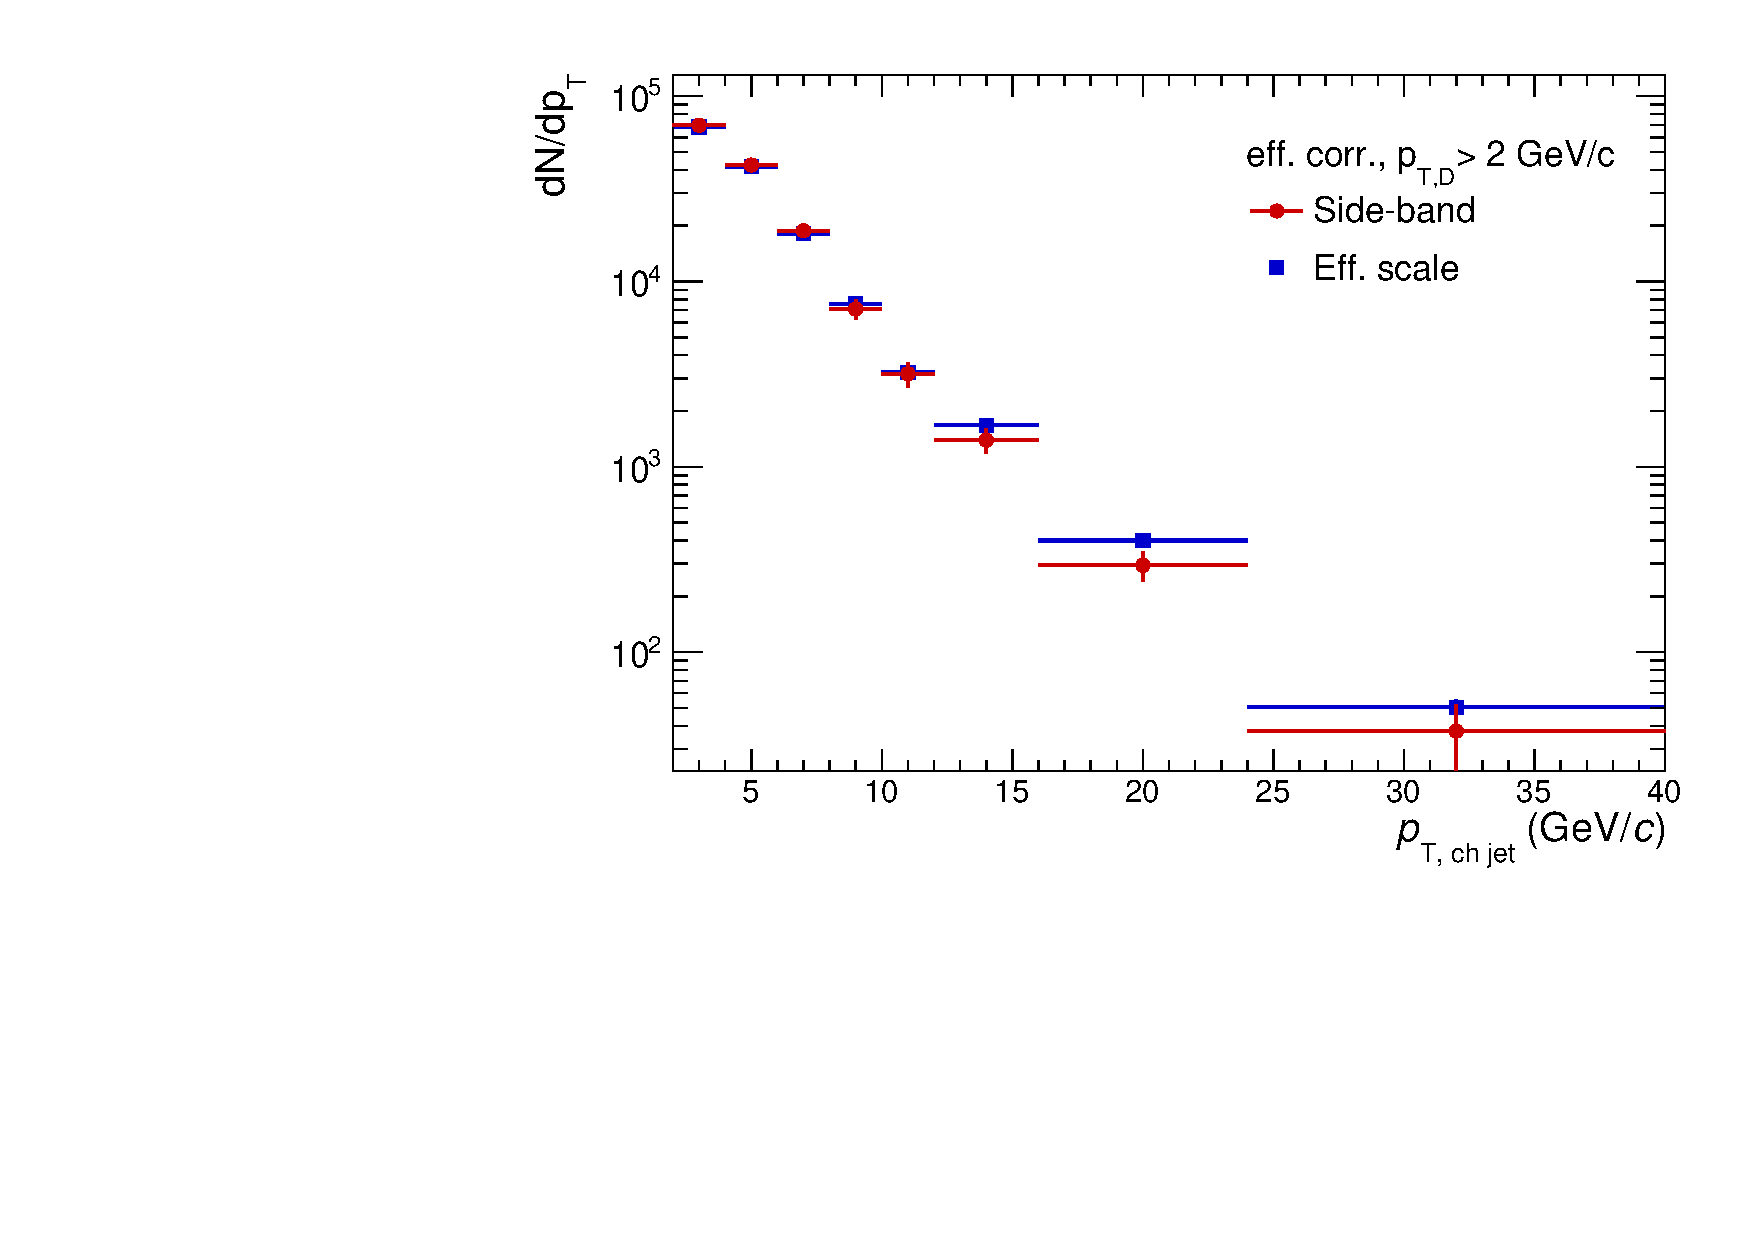
\includegraphics[width=\textwidth]{pPbplots/methodsComparison/DjetSpectra_methodComparison_FASTwoSDD_eff_ptD2}
%\caption{Yields}
%\end{subfigure}
%\begin{subfigure}[b]{0.45\textwidth}
%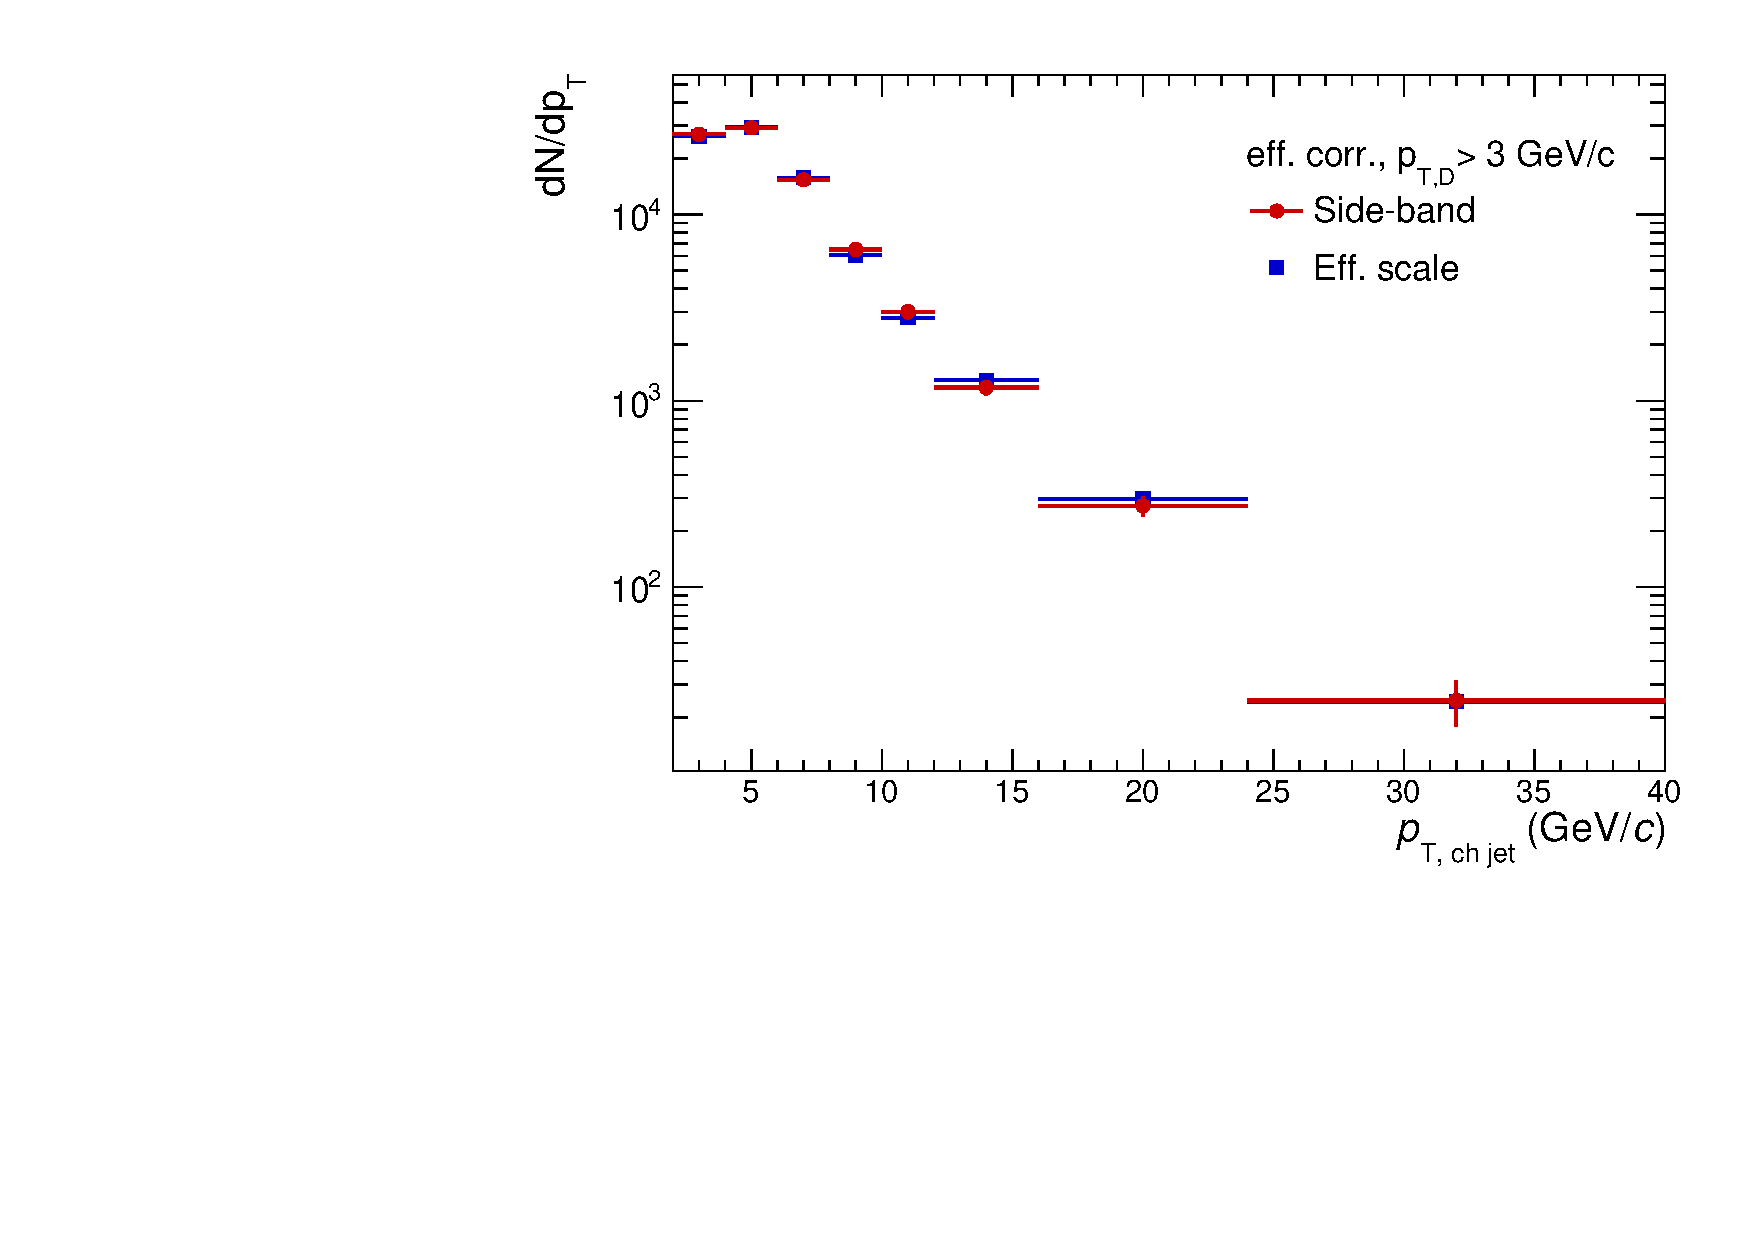
\includegraphics[width=\textwidth]{pPbplots/methodsComparison/DjetSpectra_methodComparison_FASTwoSDD_eff_ptD3}
%\caption{Yields}
%\end{subfigure}
%\begin{subfigure}[b]{0.45\textwidth}
%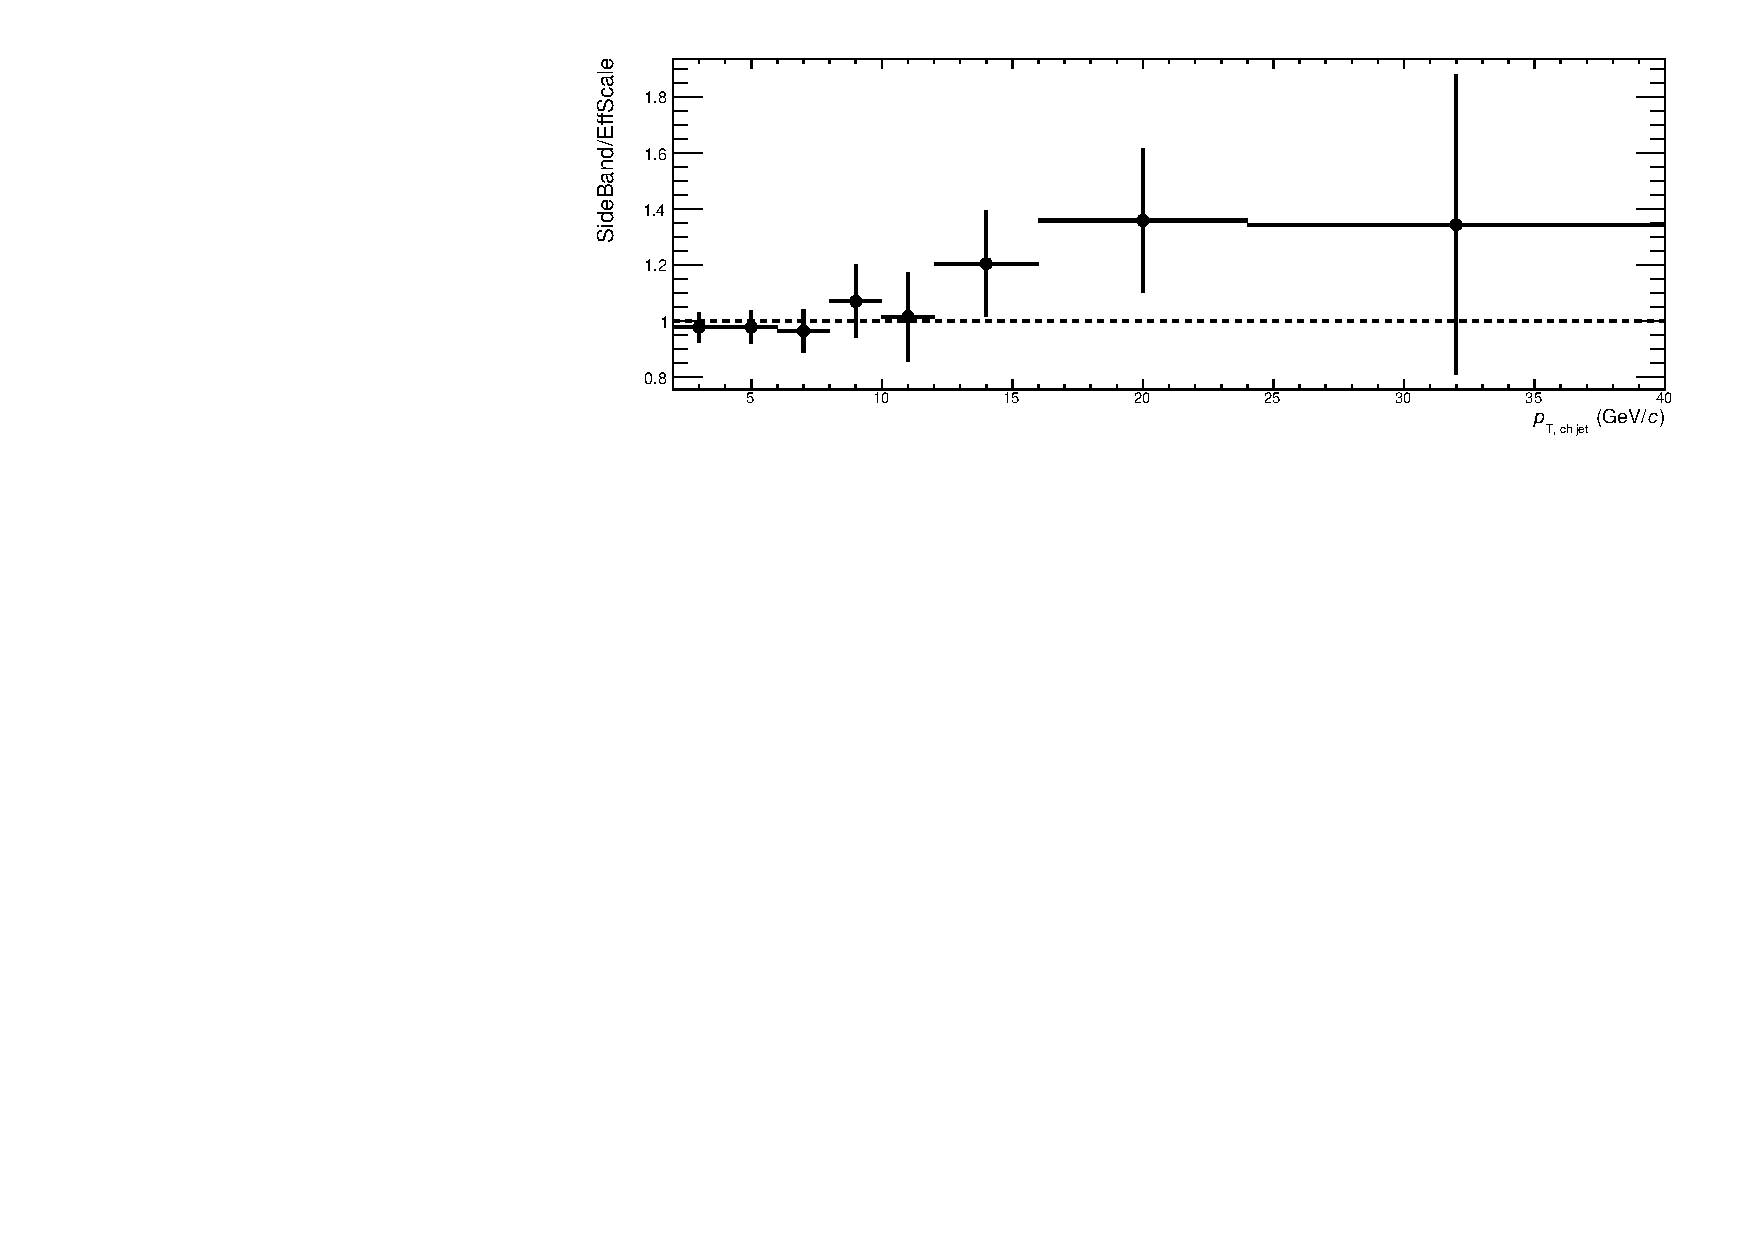
\includegraphics[width=\textwidth]{pPbplots/methodsComparison/DjetSpectraRatio_FASTwoSDD_eff_ptD2}
%\caption{Ratio}
%\end{subfigure}
%\begin{subfigure}[b]{0.45\textwidth}
%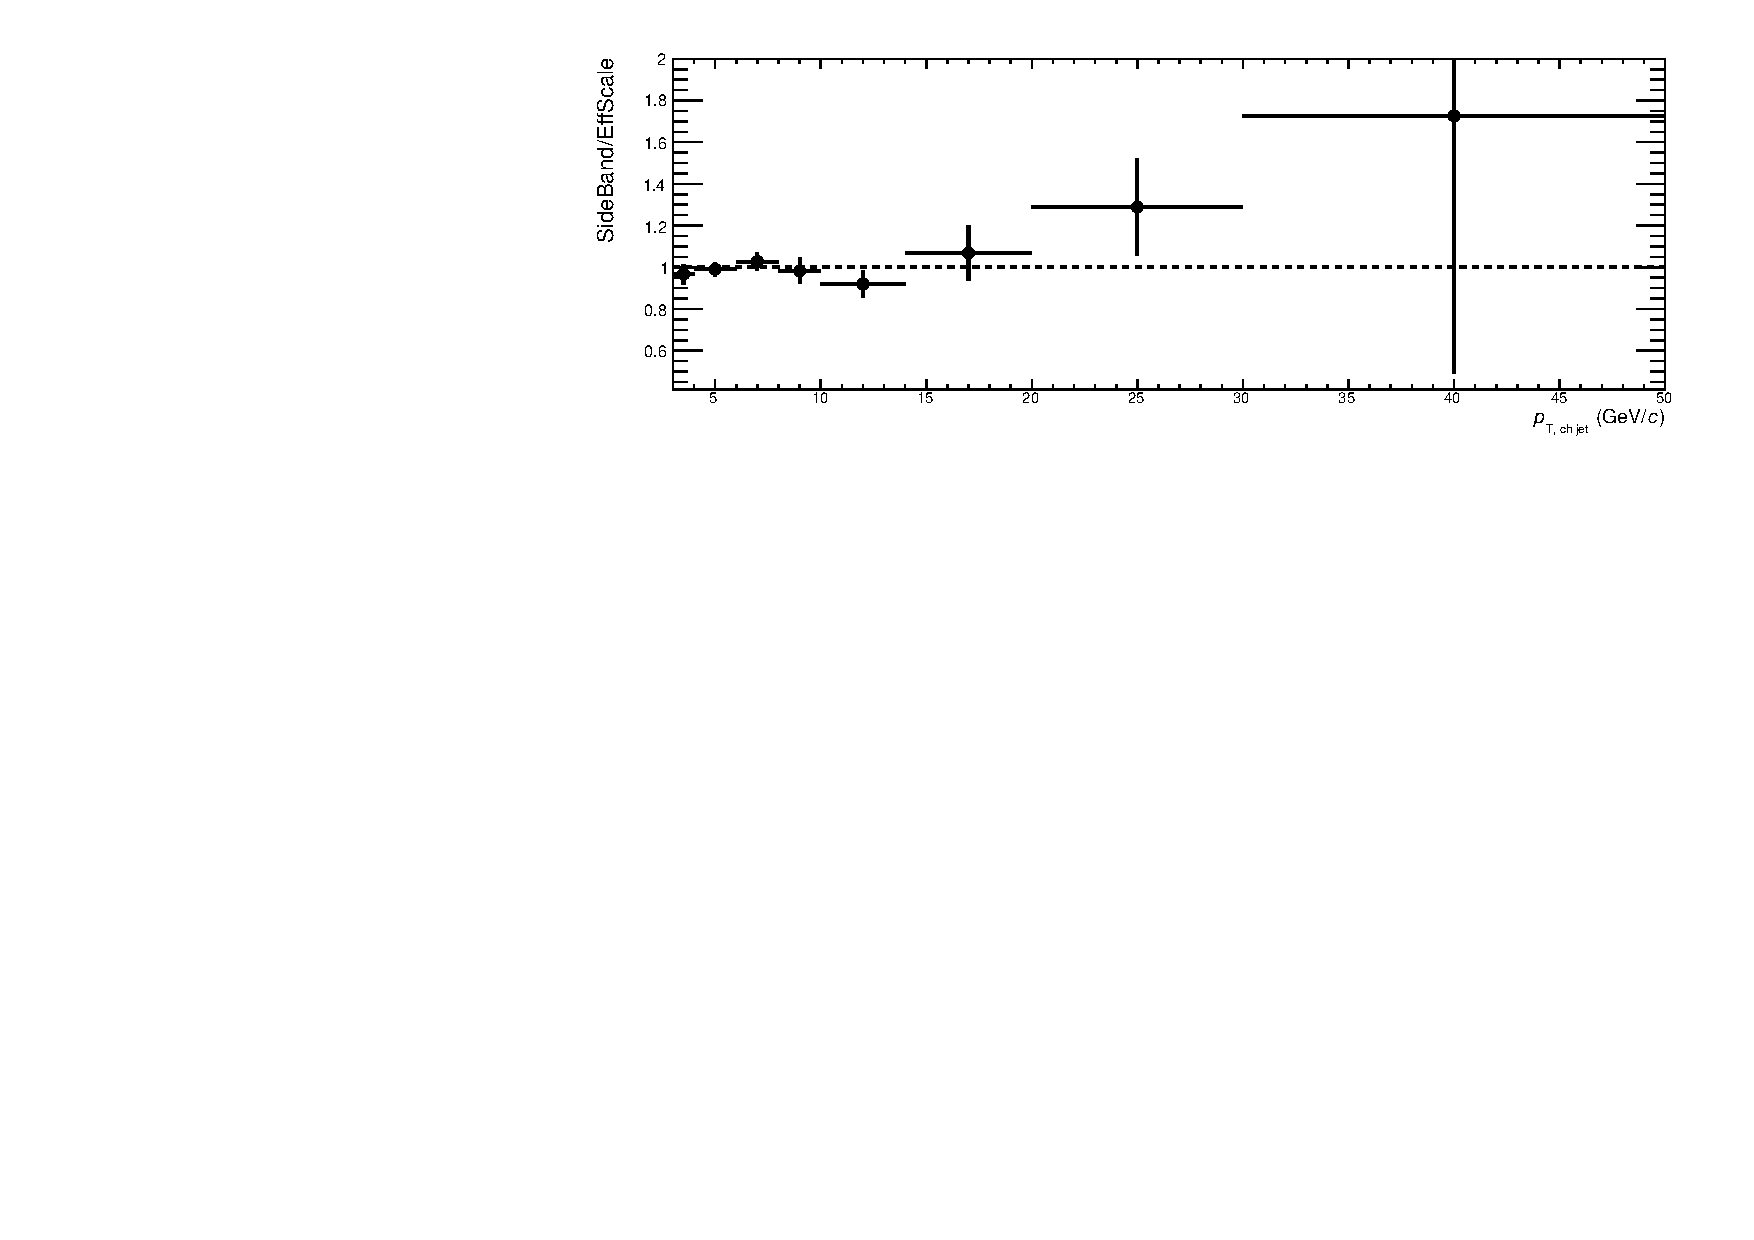
\includegraphics[width=\textwidth]{pPbplots/methodsComparison/DjetSpectraRatio_FASTwoSDD_eff_ptD3}
%\caption{Ratio}
%\end{subfigure}
%\caption{Comparison of the yields obtained using the direct jet-\pt\ extraction method and the side band subtraction method for \Dstar-jets in \pp\ at $\s=5.02$~TeV, with two cuts on \ptd: $\ptd>2$~\GeVc\ and $\ptd>3$~\GeVc.
%Reconstruction efficiency correction is applied in both cases.}
%\label{fig:JetPt_pPb_corrDrec_Dstar}
%\end{figure}
%%%Dzero
%%\begin{figure}[bth]
%%\centering
%%\begin{subfigure}[b]{0.45\textwidth}
%%\includegraphics[width=\textwidth]{pPbplotsD0/methodsComparison/}
%%\caption{Yields}
%%\end{subfigure}
%%\begin{subfigure}[b]{0.45\textwidth}
%%\includegraphics[width=\textwidth]{pPbplotsD0/methodsComparison/}
%%\caption{Yields}
%%\end{subfigure}
%%\begin{subfigure}[b]{0.45\textwidth}
%%\includegraphics[width=\textwidth]{pPbplotsD0/methodsComparison/}
%%\caption{Ratio}
%%\end{subfigure}
%%\begin{subfigure}[b]{0.45\textwidth}
%%\includegraphics[width=\textwidth]{pPbplotsD0/methodsComparison/}
%%\caption{Ratio}
%%\end{subfigure}
%%\caption{Comparison of the yields obtained using the direct jet-\pt\ extraction method and the side band subtraction method for \Dzero-jets in \pp\ at $\s=5.02$~TeV, with two cuts on \ptd: $\ptd>2$~\GeVc\ and $\ptd>3$~\GeVc.
%%Reconstruction efficiency correction is applied in both cases.}
%%\label{fig:JetPt_pPb_corrDrec_Dzero}
%%\end{figure}
%
%{\textbf{The default method used for the further analysis is the Side Band method}} with $\ptd>3$~\GeVc\ cut. The method is more stable, Gaussian fits perform better when they are done in \ptd\ bins, since in the case of the direct Jet-$p_T$ Extraction Method the different, efficiency scaled, \ptd bins are combined together which may result in non-gaussian shape of the D-meson signal. It is easier to perform the jet spectra analysis with more fine \ptchjet\ binning if needed.

%%%%%%%%%%%%%%%%%%%%%%%%%%%%%%%%%%%%%%%%%%%%%%%%%%%%%%%%%%%%%%%%%%%%%%
%%%%%%%%%%%%%%%%%%%%%%%%%%%%%%%%%%%%%%%%%%%%%%%%%%%%%%%%%%%%%%%%%%%%%%
%%%%%%%%%%%%%%%%%%%%%%%%%%%%  DETECTOR RESPONSE  %%%%%%%%%%%%%%%%%%%%%%%%%%%%
%%%%%%%%%%%%%%%%%%%%%%%%%%%%%%%%%%%%%%%%%%%%%%%%%%%%%%%%%%%%%%%%%%%%%%
%%%%%%%%%%%%%%%%%%%%%%%%%%%%%%%%%%%%%%%%%%%%%%%%%%%%%%%%%%%%%%%%%%%%%%

\section{Jet Momentum Detector Response -- Detector Response Matrix}

The detector response is studied with a Monte Carlo simulation in which particles generated by an event generator are
run through a transport code (GEANT3), that simulates the response of the detector elements, and then the same event reconstruction used in data is performed. Only \ccbar\ events are used.

Two sets of jets are obtained from the same event. One of them is obtained from the generator-level information and the second from the reconstructed signals after the detector simulation. 
The generated and reconstructed jets are matched by looking for the same D meson at both levels (using its MC label)
The detector response matrices for prompt and non-prompt are shown in Fig.~\ref{fig:fRMdet_pPb_Dzero}.

\begin{figure}[bth]
\centering
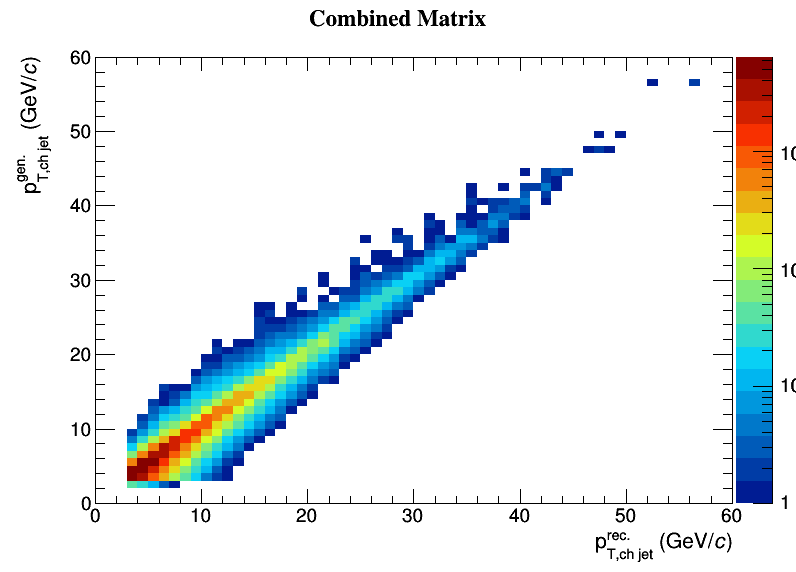
\includegraphics[width=0.45\textwidth]{pPbcuts/ProdMatrix}
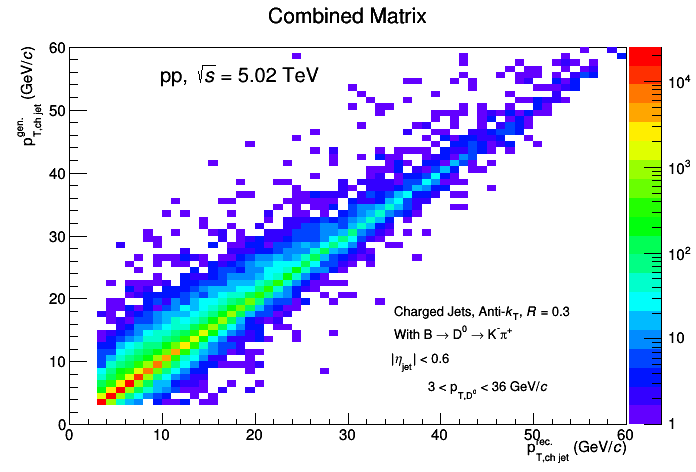
\includegraphics[width=0.45\textwidth]{pPbcuts/ProdMatrixFD}
\caption{Detector response matrix calculated with the PYTHIA part of the simulation of \pp\ events at $\s=5.02$~TeV, for prompt (left) and non-prompt (right) \Dzero-jet, R=0.3. 3 $< \ptd < $ 36~\GeVc\ .}
\label{fig:fRMdet_pPb_Dzero}
\end{figure}

The prompt detector response matrices are used to unfold the measured D-jet \pt\ spectra after subtraction of the B feed-down component. 
For each D-jet, the B feed-down is estimated based on simulations, as described later, that is folded with the presented non-prompt detector response matrix.
%
%Figure~\ref{fig:pPb_ResponseMatrixProj} shows projections of the response on the detector level jet \pt\ in bins of a particle level jet \pt.
%
%\begin{figure}[bth]
%\centering
%\includegraphics[width=0.9\textwidth]{pPbplots/ResponseMatrix/DetMatrixProjectionsComparison_Dpt3_36}
%\caption{Projections of the response on the detector level jet \pt\ in bins of a particle level jet \pt\ calculated with the Pythia simulation of \pp\ events at $\s=5.02$~TeV.}
%\label{fig:pPb_ResponseMatrixProj}
%\end{figure}
%
%\subsection{Jet Momentum Resolution}
%
%The jet momentum resolution and energy scale shift are estimated calculating the variable:
%\begin{equation}
%(p_{\mathrm{T,ch\, jet}}^{\mathrm{det}} - p_{\mathrm{T,ch\, jet}}^{\mathrm{part}}) / p_{\mathrm{T,ch\, jet}}^{\mathrm{part}}
%\label{eq:detResp}
%\end{equation}
%for each matched pair of a particle-level jet with a detector-level jet.
%Figure~\ref{fig:pPb_DetectorResponse} shows the probability density distribution of Eq.~\ref{eq:detResp} for \Dstar-jets in \pp\ collisions at $\s=5.02$~TeV.
%
%\begin{figure}[bth]
%\centering
%\includegraphics[width=0.9\textwidth]{pPbplots/ResponseMatrix/DetMatrixResProjectionsComparison}
%\caption{Jet momentum resolution calculated with a full simulation of \pp\ events at $\s=5.02$~TeV.}
%\label{fig:pPb_DetectorResponse}
%\end{figure}
%
%Figure~\ref{fig:pPb_ResponseMatrixProj} and~\ref{fig:pPb_DetectorResponse} include also a comparison of responses for prompt (red) and non-prompt (blue) \Dstar-jet\ production. The non-prompt response is used at the B feed-down subtraction level, as described in~\ref{sect:FD}.
%


%%%%%%%%%%%%%%%%%%%%%%%%%%%%%%%%%%%%%%%%%%%%%%%%%%%%%%%%%%%%%%%%%%%%%%
%%%%%%%%%%%%%%%%%%%%%%%%%%%%%%%%%%%%%%%%%%%%%%%%%%%%%%%%%%%%%%%%%%%%%%
%%%%%%%%%%%          FEED-DOWN            %%%%%%%%%%%%%%%%%%%%%%%%%%%%
%%%%%%%%%%%%%%%%%%%%%%%%%%%%%%%%%%%%%%%%%%%%%%%%%%%%%%%%%%%%%%%%%%%%%%
%%%%%%%%%%%%%%%%%%%%%%%%%%%%%%%%%%%%%%%%%%%%%%%%%%%%%%%%%%%%%%%%%%%%%%

\section{Feed-Down Correction}
\label{sec:FD}

A fraction of the measured D mesons originates from the decays of B mesons. These D mesons are usually referred to as non-prompt,
to distinguish them from the prompt fraction, i.e. the ones that come directly from the fragmentation of a charm quark or decays of higher excited charm states.
The longer decay length of B mesons combined with the topological cuts applied in the D meson selection causes the reconstruction efficiency 
to be higher for the non-prompt fraction compared to the prompt fraction. This is shown in Fig.~\ref{fig:eq_pp_DrecEff}.
As a consequence, the natural admixture of the prompt and non-prompt $D-jets$ is biased in a detector-specific way towards the non-prompt.
In order to make meaningful comparisons with theoretical and other experimental results one needs to either correct the bias or remove completely the non-prompt fraction and report only the prompt fraction. 
Both approaches require to use theoretical models or Monte Carlo simulations.
In ALICE the second approach has been preferred so far, and for this analysis we decided to follow it.

\subsection{Monte Carlo Simulation}

For the D-meson spectra analysis, ALICE has used FONLL~\cite{Cacciari:1998} calculations to estimate the non-prompt fraction~\cite{ALICE:2012d, ALICE:2014d, ALICE:2016a}.
In this analysis however we need to extract the B feed-down fraction also as a function of the jet kinematics, therefore this approach is not applicable.
We decided to use POWHEG~\cite{Alioli:2010}, a Monte Carlo event generator known to reasonably reproduce FONLL calculations and previous experimental results~\cite{Cacciari:2012b}.
The second part of the parton shower and the fragmentation into hadrons is provided by PYTHIA6 (Perugia-2011 tune).

We generated 25 M \bbbar\ events for the baseline parameters: 
$m_{\rm b} = 4.75$~\GeVcsq, $\mu_{\rm R} = \mu_{\rm F} =\mu_{0} = \sqrt{m^2+\pt^2}$,
where $m_{\rm b}$ is the beauty masses, $\mu_{\rm R}$ and $\mu_{\rm F}$ are respectively the renormalization and factorization scale factors; used based PDF set is: CT10NLO.
Variation of the simulation parameters are a source of the B feed-down subtraction systematic uncertainties.

The reconstruction of D-meson jets is performed in the POWHEG+PYTHIA6 events using the same procedure used for the main data analysis.

\subsection{Feed-Down Subtraction}
The B feed-down (FD) is subtracted from the measured D-meson jet \pt\ spectra by scaling the cross-section of D-meson jets obtained from the analysis of the POWHEG+PYTHIA simulation by the integrated luminosity of the analyzed data, according to Eq.~\ref{eq:bFDsub}:
\begin{equation}
N^{\rm c\rightarrow\Dstar}(\ptchjetdet) = 
N^{\rm c,b\rightarrow\Dstar}(\ptchjetdet) - 
R_{\rm det}^{\rm b\rightarrow\Dstar}(\ptchjetdet,\ptchjetgen) \otimes \sum_{\ptd} \frac{\epsilon^{\rm b\rightarrow\Dstar}(\ptd)}{\epsilon^{\rm c\rightarrow\Dstar}(\ptd)} N^{\rm b\rightarrow\Dstar}_{\rm POWHEG}(\ptd,\ptchjetgen),
\label{eq:bFDsub}
\end{equation}
where:
\begin{itemize}
\item $N^{\rm c\rightarrow\Dstar}(\ptchjetdet)$ is the efficiency-corrected measured yield after FD subtraction; 
\item $N^{\rm c,b\rightarrow\Dstar}(\ptchjetdet)$ is the efficiency-corrected measured yield before FD subtraction;
\item $R_{\rm det}^{\rm b\rightarrow\Dstar}(\ptchjetdet,\ptchjetgen)$ is the detector response matrix of the \pt\ of non-prompt \Dzero-jets;
\item the symbol $\otimes$ is to be interpreted as the standard product of the response matrix times the vector of the yields in bins of \ptchjetgen;
\item $\epsilon^{\rm c\rightarrow\Dstar}(\ptd)$ and $\epsilon^{\rm b\rightarrow\Dstar}(\ptd)$ are respectively the reconstruction efficiencies of prompt and non-prompt \Dzero\ mesons;
\item $N^{\rm b\rightarrow\Dstar}_{\rm POWHEG}(\ptd,\ptchjetgen)$ is the cross-section of \Dstar-jets from the POWHEG simulation scaled by the integrated luminosity of the analyzed data.
\end{itemize}
Since the measured yields are corrected for the prompt D-jet efficiency, the The POWHEG D-jet spectrum is weighted with the ratio of the non-prompt over the prompt D-jet efficiency in D-meson \pt\ bins.

%Projections of prompt and non-prompt \Dstar-jets response matrices in slices \ptchjetgen are shown in Fig.~\ref{fig:pPbres_prompt_nonprompt}. There are small differences between the prompt and non-prompt response seen. 
There are differences between the prompt and non-prompt response, for this reason the FD has to be subtracted before unfolding the measured spectrum; furthermore, as illustrated in Eq.~\ref{eq:bFDsub}, the spectrum obtained from the POWHEG simulation is smeared using the response of non-prompt D-jets. 
Figure~\ref{fig:pPbFD_corr_Dzero} compares the measured \Dzero-jet \pt\ spectrum with the FD spectrum and the subtracted spectrum.


\begin{figure}[bth]
\centering
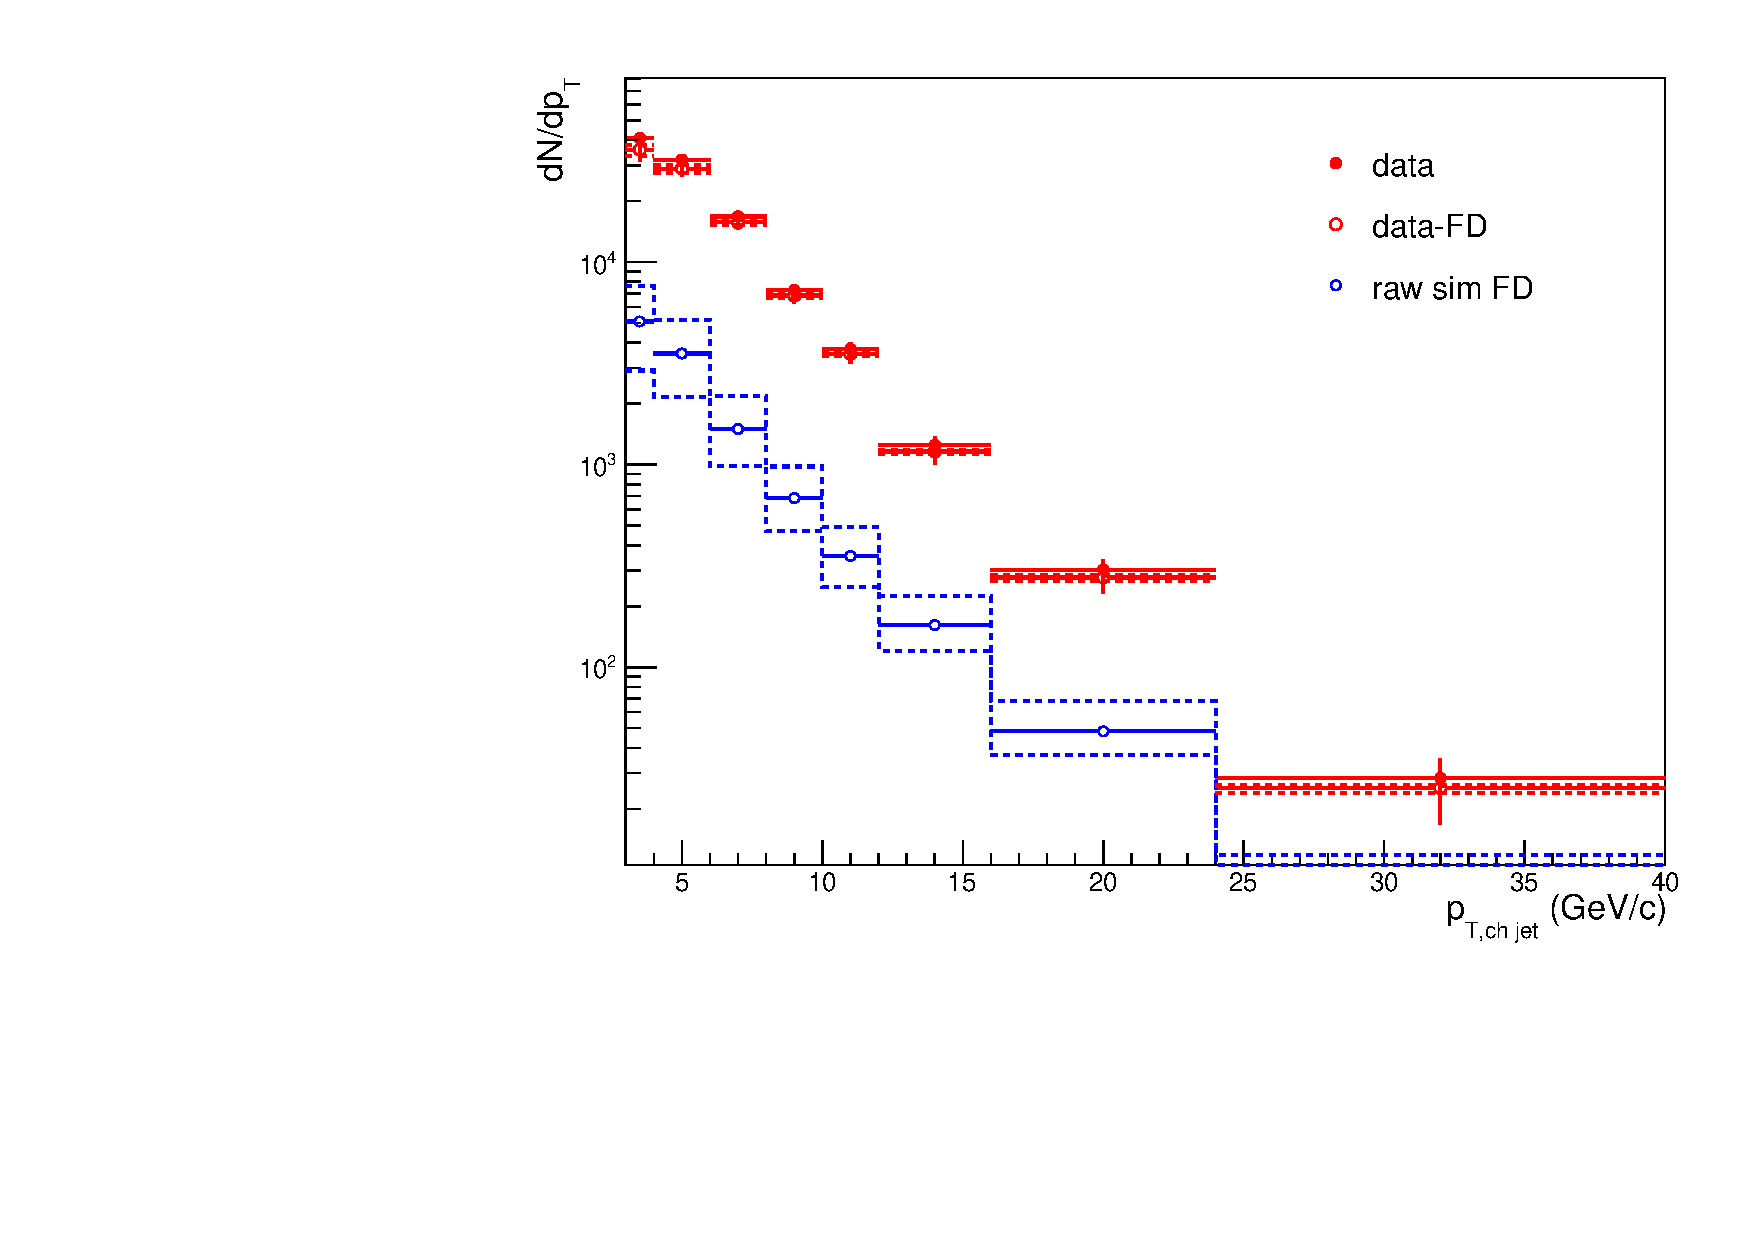
\includegraphics[width=.45\textwidth]{pPbcuts/JetPtSpectra_FDsub}
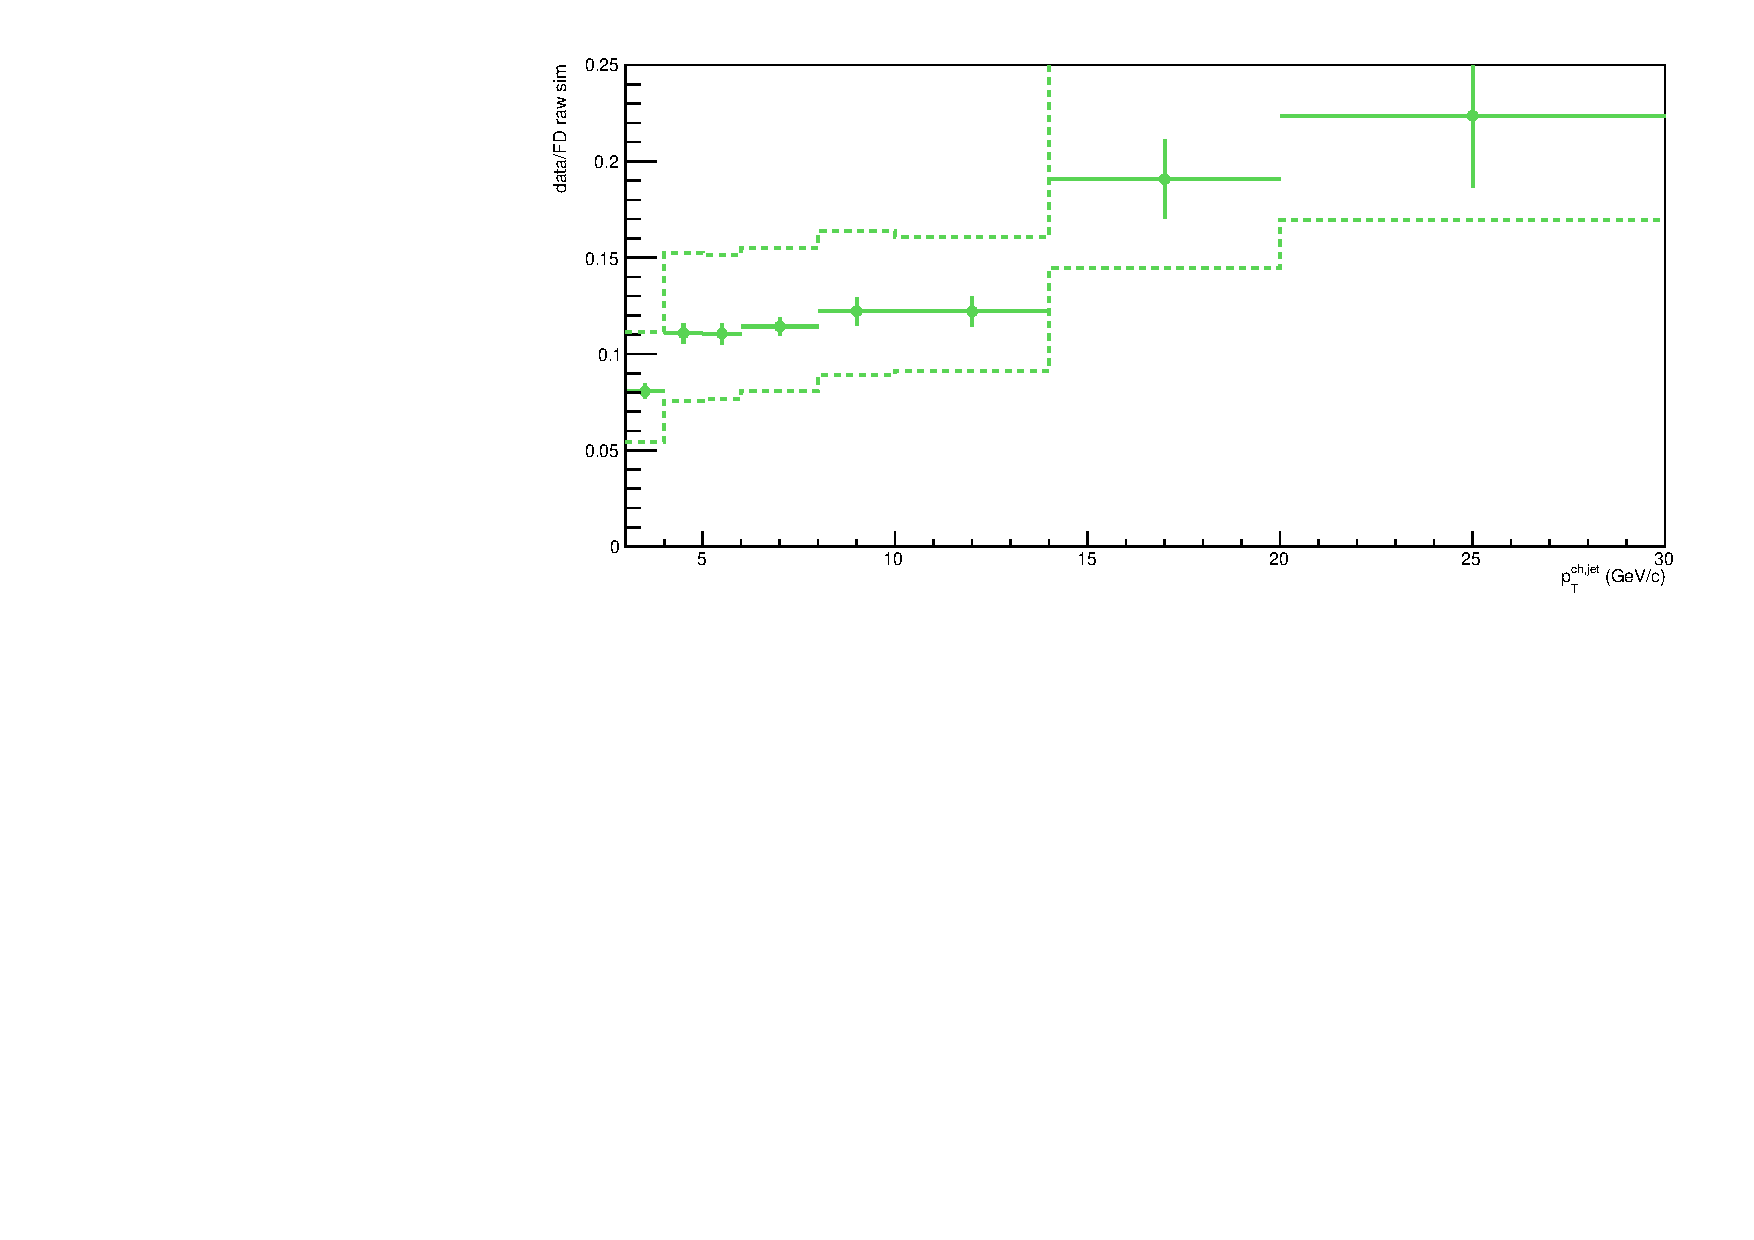
\includegraphics[width=.45\textwidth]{pPbcuts/FDratio}
\caption{Left: Efficiency-corrected measured \Dzero-jet spectrum in \pp\ collisions at $\s=5.02$~TeV before FD correction (green) and after FD correction (red). The FD spectrum is also plotted (blue) with its uncertainties. Right plot shows ratio of non-prompt to inclusive \Dzero-jet spectrum.}
\label{fig:pPbFD_corr_Dzero}
\end{figure}


%%%%%%%%%%%%%%%%%%%%%%%%%%%%%%%%%%%%%%%%%%%%%%%%%%%%%%%%%%%%%%%%%%%%%%
%%%%%%%%%%%%%%%%%%%%%%%%%%%%%%%%%%%%%%%%%%%%%%%%%%%%%%%%%%%%%%%%%%%%%%
%%%%%%%%%%%%         UNFOLDING            %%%%%%%%%%%%%%%%%%%%%%%%%%%%
%%%%%%%%%%%%%%%%%%%%%%%%%%%%%%%%%%%%%%%%%%%%%%%%%%%%%%%%%%%%%%%%%%%%%%
%%%%%%%%%%%%%%%%%%%%%%%%%%%%%%%%%%%%%%%%%%%%%%%%%%%%%%%%%%%%%%%%%%%%%%

\section{Unfolding}
\label{sect:unfResults}

Due to detector finite momentum resolution and tracking inefficiency the jet \pt\ spectra measured as described
in the previous sections are distorted. These distortions are detector-specific and do not allow a direct comparison
with theoretical models and other independent experimental results.
In order to correct for these distortions, we first need to assess the detector performance and quantify
the detector response to the D-meson jets. 
Then the matrix is rebinned according to the binning used for the final jet \pt\ spectra. The detector response matrix, a distribution used as a prior and the corrected jet \pt\ spectrum obtained from the data are passed to the unfolding algorithm. The algorithm returns an unfolded jet \pt\ spectrum. As a prior, the spectrum obtained from the Monte Carlo simulation at the generator level is used.


\subsection{\Dzero-tagged jets}

Figure~\ref{fig:pPb_ResponseMatrix_Dzero} shows a rebinned response matrix for prompt \Dzero-jets.
The corrected for the reconstruction efficiency and B feed-down jet \pt\ spectra before the unfolding (blue) and after the unfolding (red), for the side-band method, are presented in Fig.~\ref{fig:UnfSpec_pPb_Dzero}.
Unfolding is done with Bayesian technique using the \texttt{RooUnfold} software package. The default method is the Bayesian with 4 iterations and \ptchjet\ ranges are 3 $< \ptchjet< $ 50 both for the generator and reconstructed level \pt\, with over/under flow bins considered in the unfolding procedure.
The green line represents refolded back spectrum, and is compared to the measured jet spectrum before unfolding with different iterations in the Bayes unfolding - right panel of Fig.~\ref{fig:unfIterations_pPb_Dzero}. Figure~\ref{fig:unfIterations_pPb_Dzero} (left) shows also unfolded spectra with next iterations compared to the default spectrum obtained with 4 iterations.
The final reported jet \pt\ range is 5 $< \ptchjet<$ 50 GeV/$c$.
Comparison of unfolded spectra with the SVD method, different \pt\ ranges for the input and unfolded spectra, and different priors are presented in the systematic uncertainties section, see~\ref{sUnfoldSys}. 

\begin{figure}[bth]
\centering
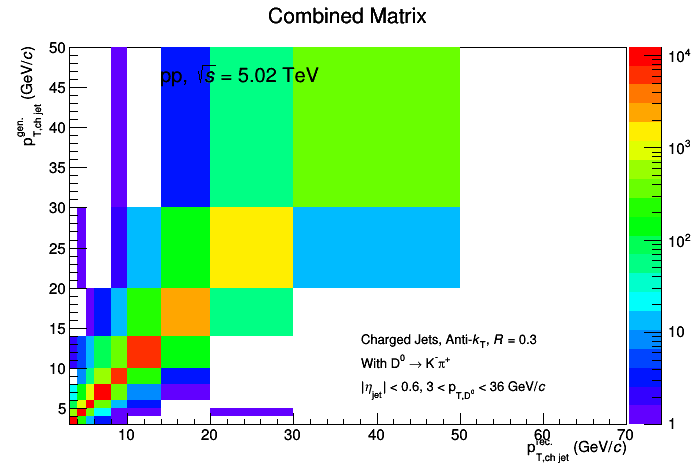
\includegraphics[width=0.7\textwidth]{pPbcuts/ProdMatrixRebin}
\caption{Rebinned detector response matrix for prompt \Dzero-jet in \pp\ events at $\s=5.02$~TeV, with R=0.3.}
\label{fig:pPb_ResponseMatrix_Dzero}
\end{figure}

\begin{figure}[bth]
\centering
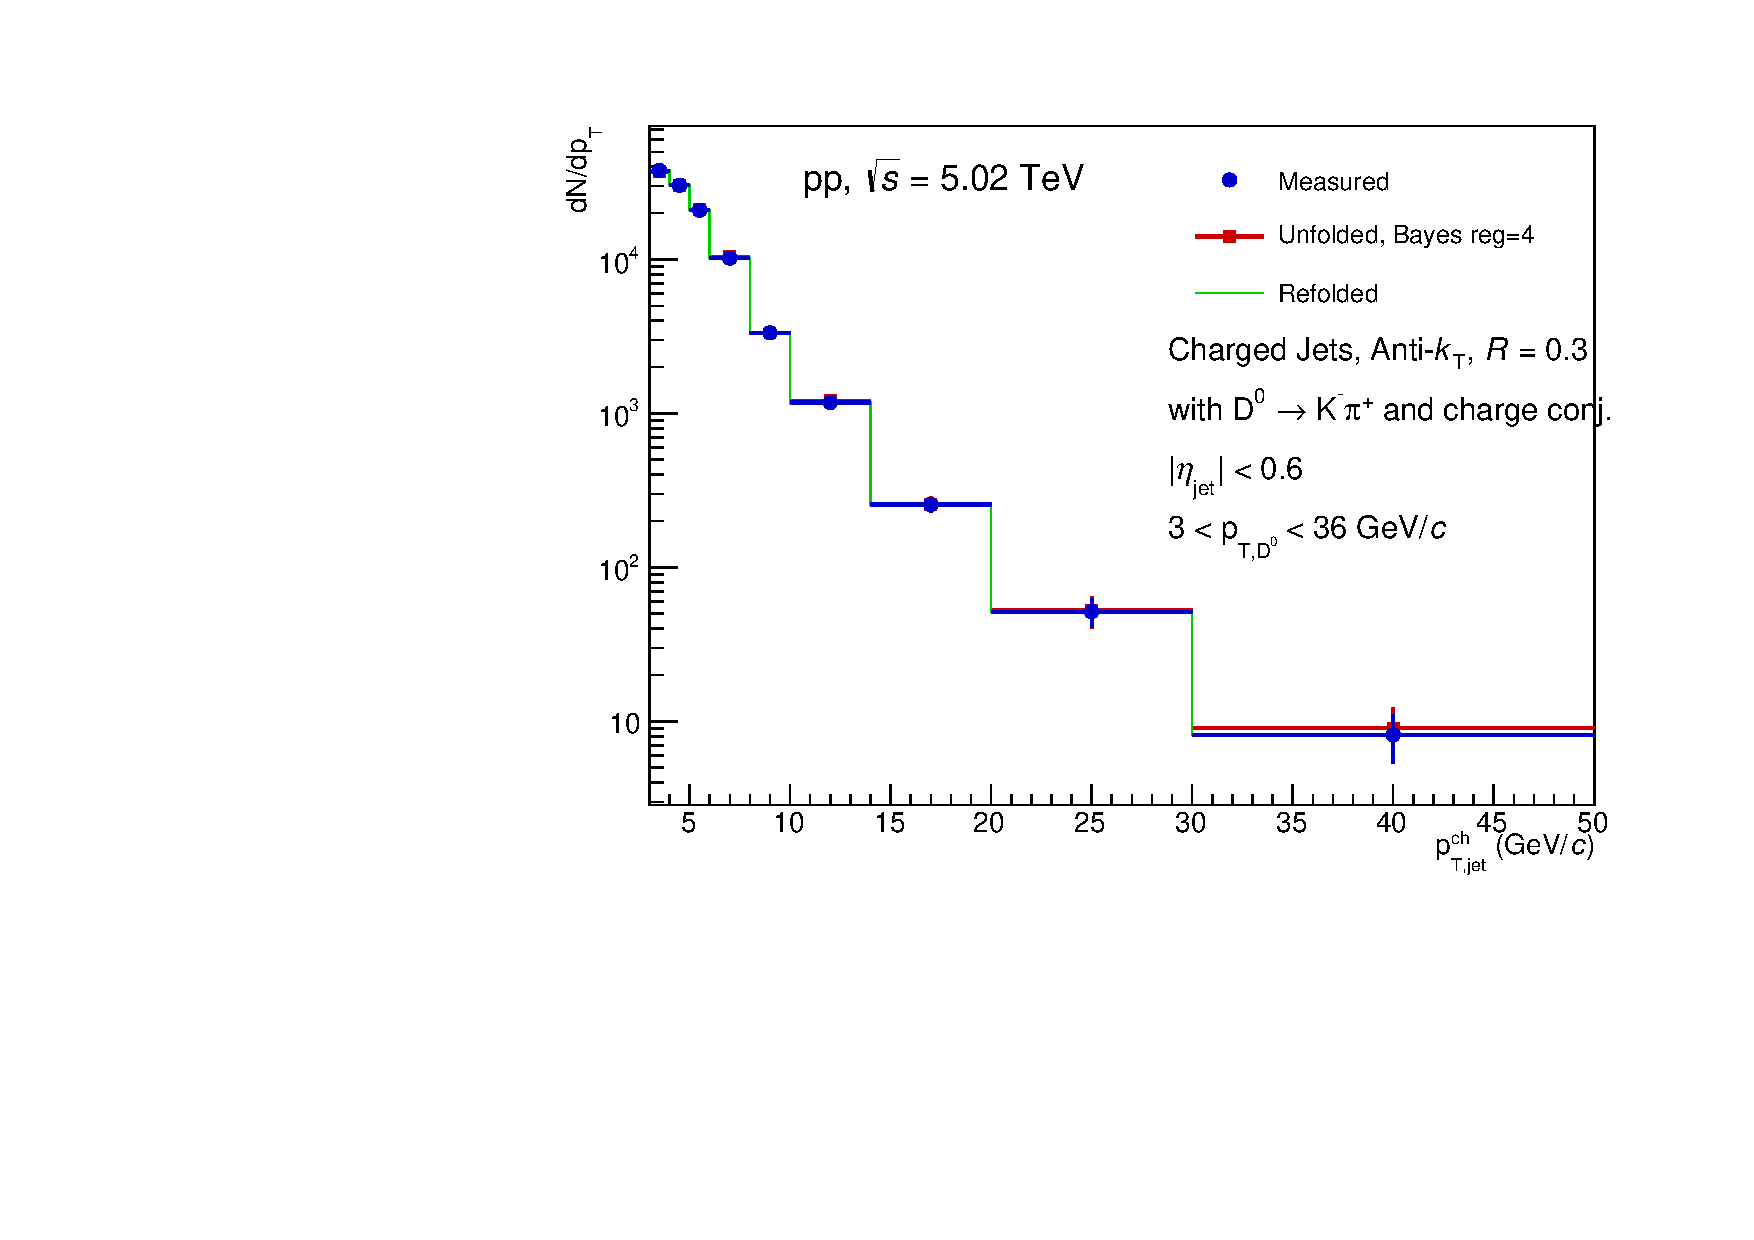
\includegraphics[width=0.55\textwidth]{pPbcuts/unfoldedSpectrum_UnfSpectrum}
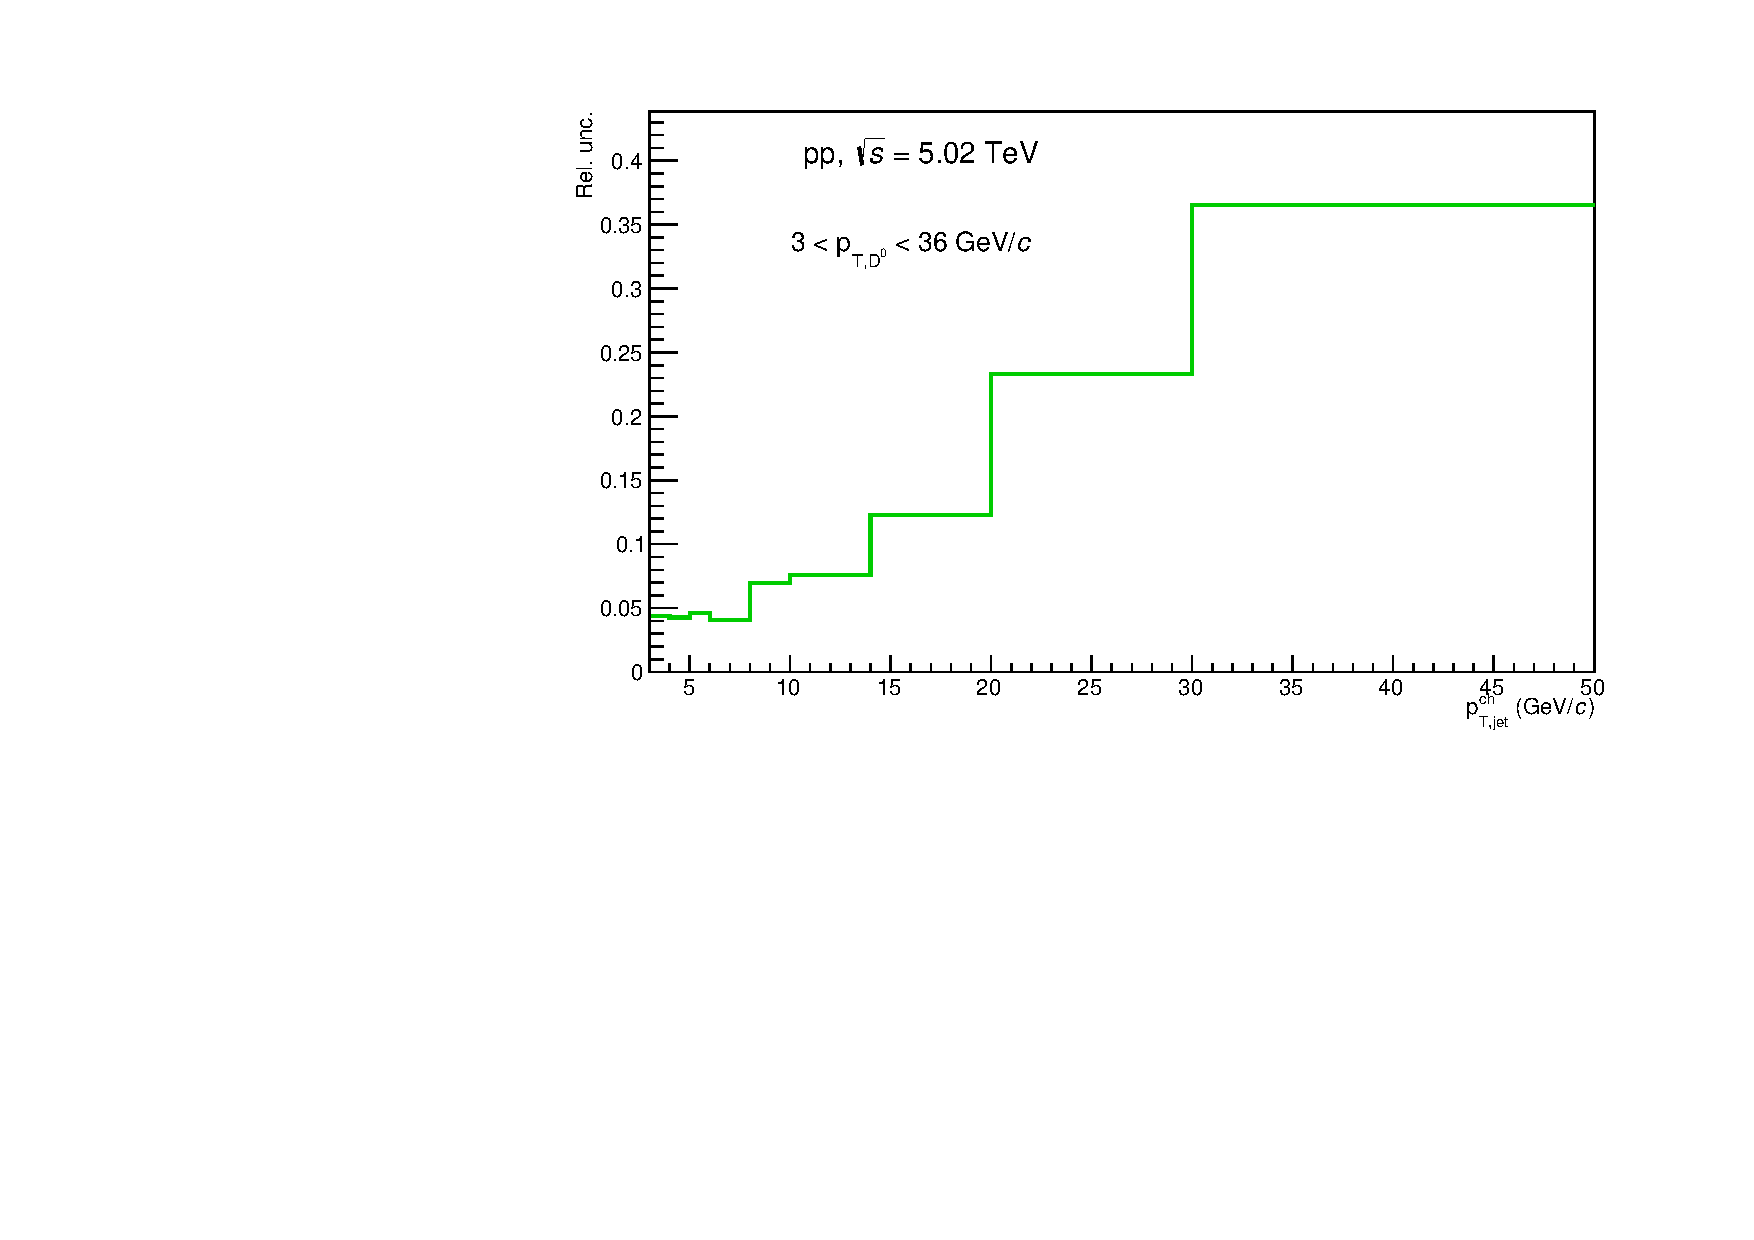
\includegraphics[width=0.4\textwidth]{pPbcuts/unfoldedSpectrum_UnfSpectrum_unc}
\caption{Left: Corrected jet \pt spectrum before (blue) and after (red) the unfolding procedure (Bayesian method with 4 iterations), \pp\ events at $\s=5.02$~TeV. Right: Relative statistical uncertainties on the \Dzero-tagged jet \pt\ spectrum after unfolding.}
\label{fig:UnfSpec_pPb_Dzero}
\end{figure}

\begin{figure}[bth]
\centering
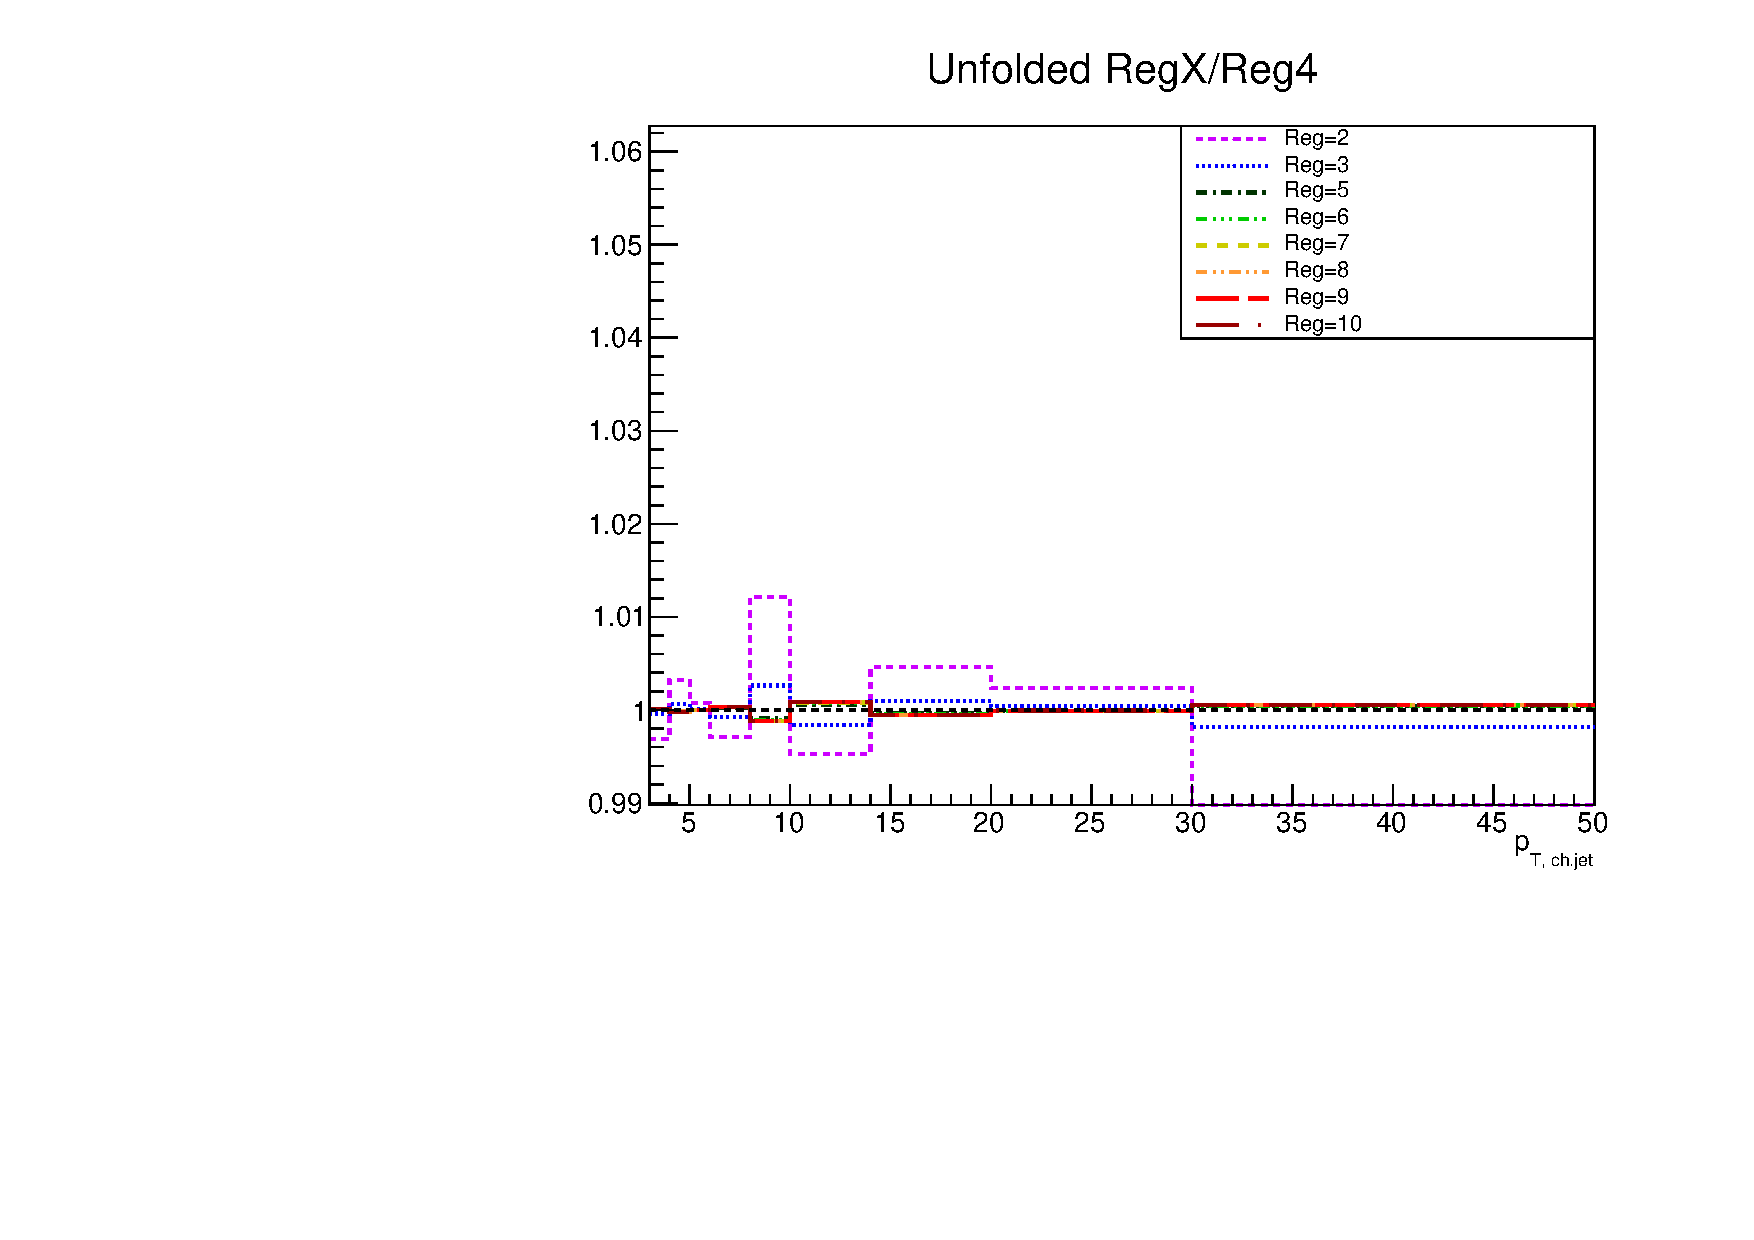
\includegraphics[width=0.45\textwidth]{pPbcuts/unfoldedSpectrum_unfRatio}
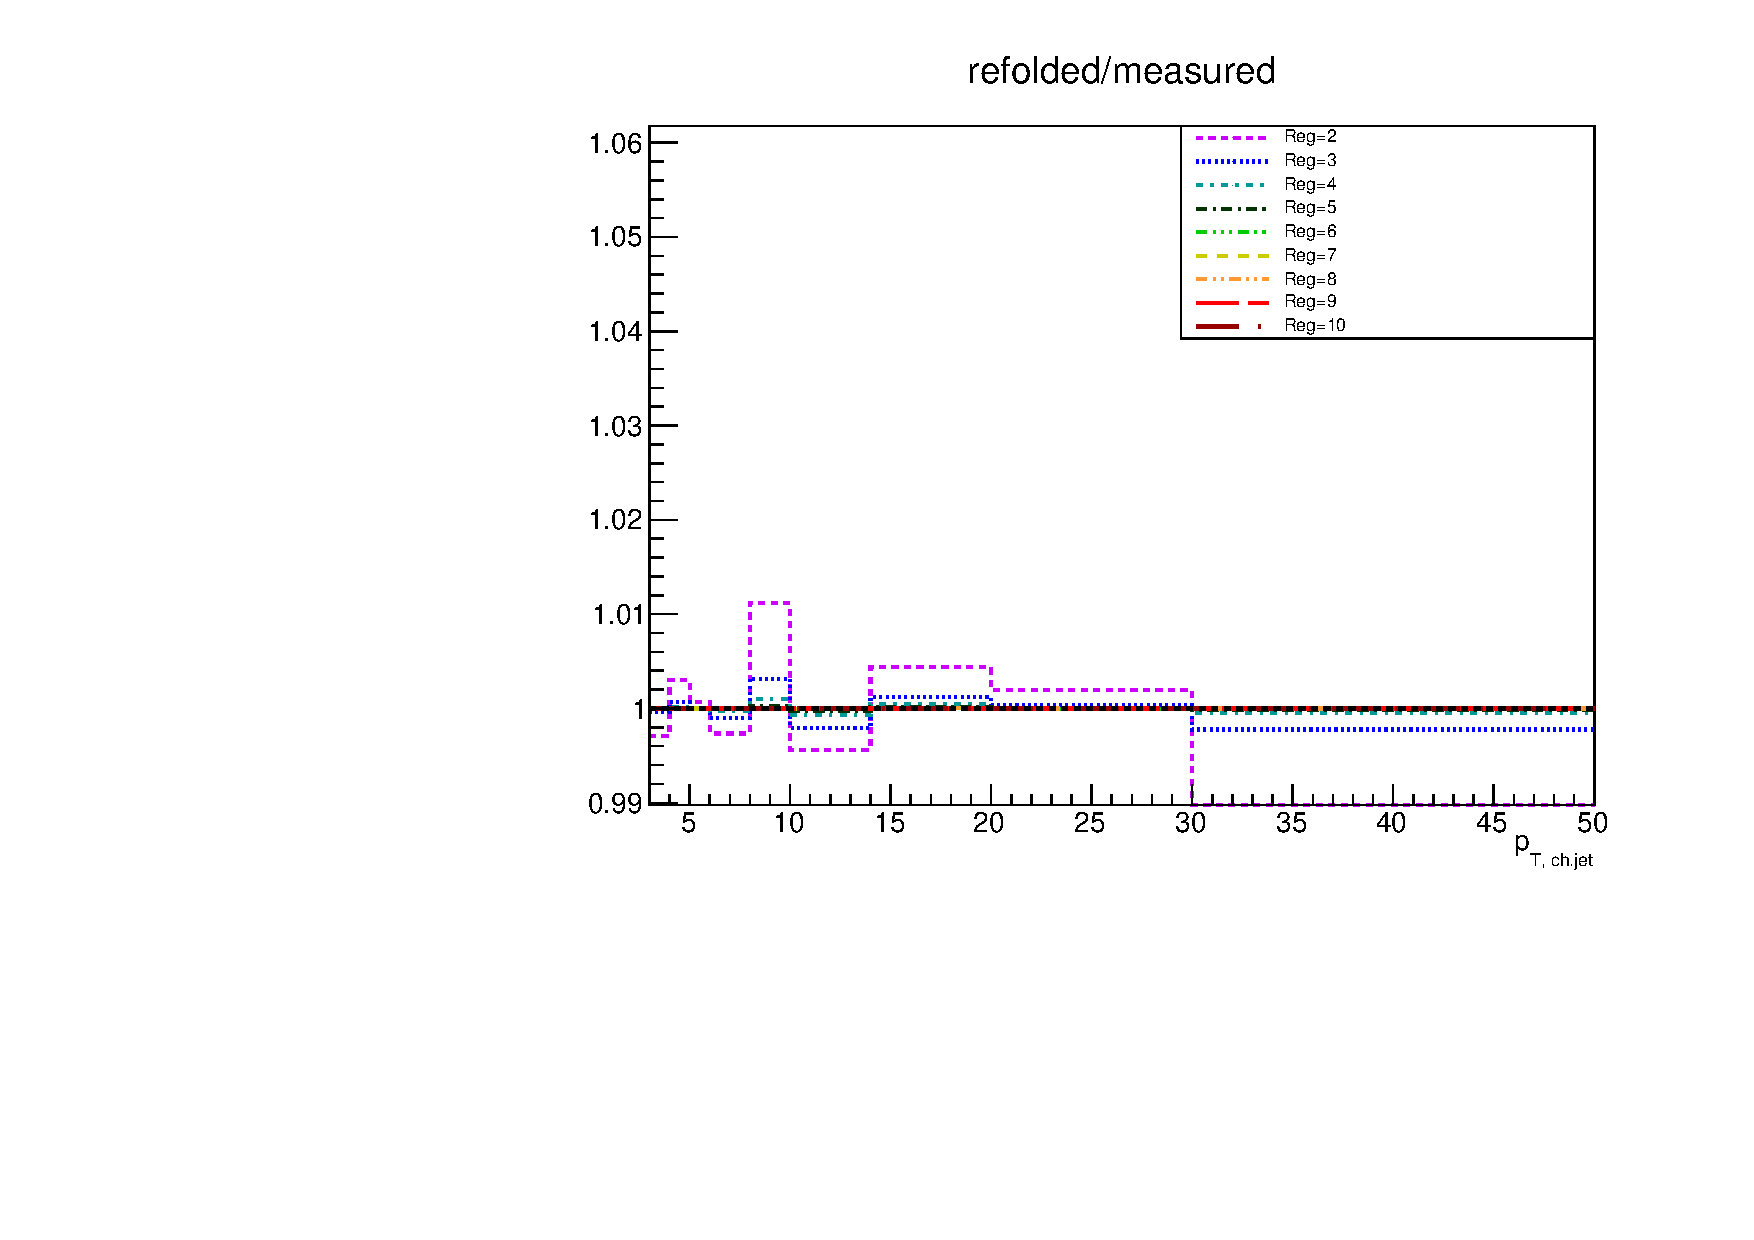
\includegraphics[width=0.45\textwidth]{pPbcuts/unfoldedSpectrum_foldedRatio}
\caption{Left: ratio of the unfolded spectra for up to 10 iterations to the default unfolded spectrum with 4 iterations in the Bayesian unfolding. Right: ratio of the refolded spectrum for up to 10 iterations to the measured in the Bayesian unfolding. The considered jet \pt\ range is above 5 GeV/$c$.}
\label{fig:unfIterations_pPb_Dzero}
\end{figure}

\begin{figure}[bth]
\centering
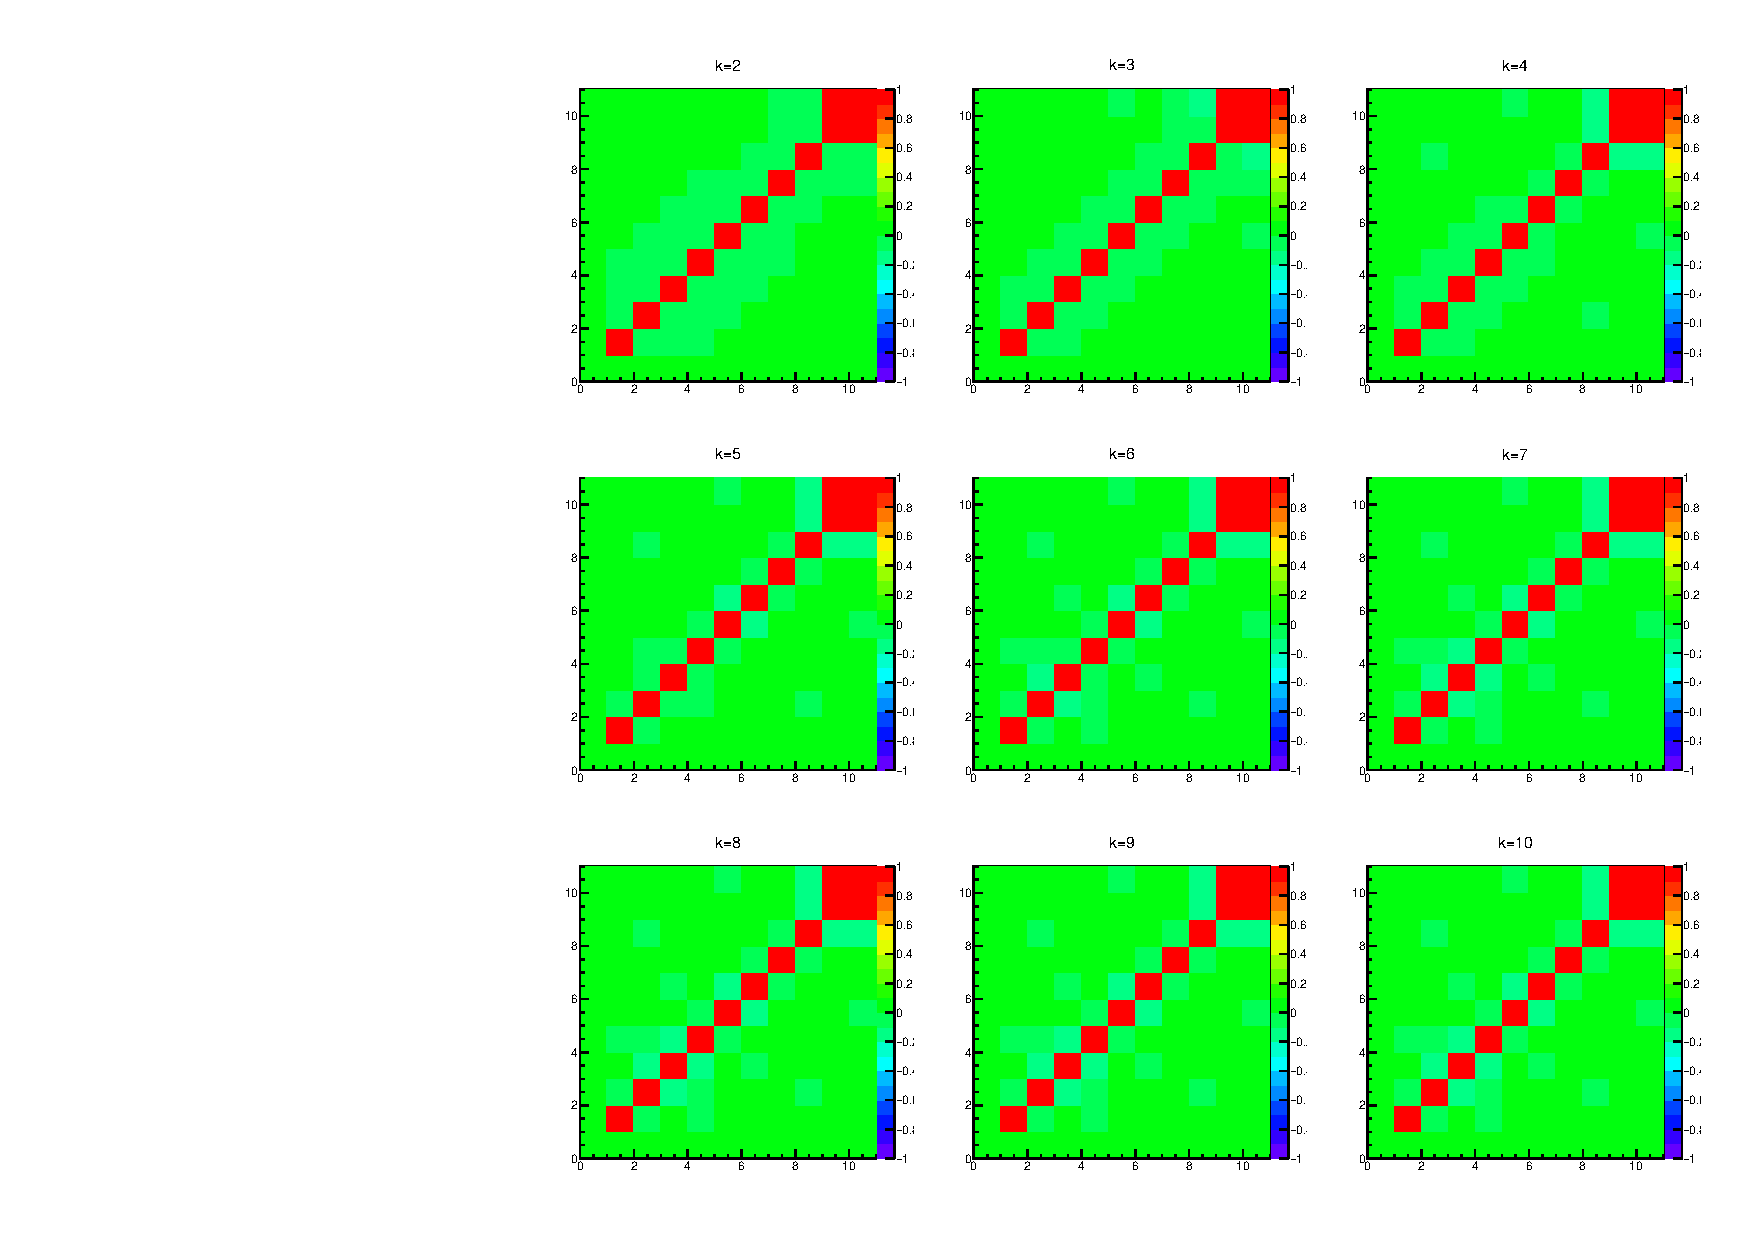
\includegraphics[width=0.8\textwidth]{pPbcuts/unfoldedSpectrum_Pearson}
\caption{Pearson coefficients for Bayesian unfolding.}
\label{fig:unfIterations_pPb_Dzero}
\end{figure}

\section{Systematic Uncertainties}

We considered the following sources of systematic uncertainties:

\begin{easylist}[itemize]
& Raw yield extraction
& D-Meson Selection Cuts
& B Feed-Down
& Unfolding
& Tracking Efficiency
& \pt\ Shape of the Monte Carlo Spectrum
\end{easylist}

\subsection{Raw Yield Extraction}

\subsubsection{Fitting procedure}
The stability and systematics of the raw yield extraction has been assessed using the \texttt{MultiTrial} framework developed by the D2H group.
This framework performs the fit of the invariant mass distribution many times varying several conditions, such us binning, fixed vs. free parameters,
background function, fit range.

The following variations were included in the assessment of the systematics for the raw yield extraction of \Dzero jets in \pp:
\begin{itemize}
\item fixed $\sigma=\sigma_{\rm MC}$;
\item fixed $\sigma=1.15\sigma_{\rm MC}$
\item fixed $\sigma=0.85\sigma_{\rm MC}$
\item free $\sigma$ and fixed $m_{0}=m_{\rm PDG}$;
\item fixed $\sigma=\sigma_{\rm MC}$ and $m_{0}=m_{\rm PDG}$;
\item free $\sigma$ and free $m_{0}$;
\item background functions: exponential, linear, second-order polynomial;
\item lower limit of fit range: $1.72$, $1.74$~\GeVcsq;
\item upper limit of fit range: $2.00$, $2.03$~\GeVcsq;
\item rebin by factor 2
\end{itemize}

Figure~\ref{fig:MultiTrialSB_trials_pPB_Dzero} shows average of the multi-trial procedure for the side-band method as a function of jet \pt\ for each \Dzero \pt\ bin scaled by the corresponding efficiency, and average of the all \Dzero\ \pt\ bins (blue). 
Variations of all trials as a function of jet \pt\ for each \Dzero\ \pt\ bin and scaled by the corresponding efficiency are shown in Fig~\ref{fig:MultiTrialSB_allDptVairations_pPB_Dzero}.

\begin{figure}[bth]
\begin{center}

\includegraphics[width=0.3\textwidth]{missing}

\includegraphics[width=0.3\textwidth]{missing}
\caption{Average of the multi-trial procedure for the side-band method as a function of jet \pt\ for each \Dzero\ \pt\ bin scaled by the corresponding efficiency, and average of the all \Dzero\ \pt\ bins (blue).} 
\label{fig:MultiTrialSB_trials_pPB_Dzero}
\end{center}
\end{figure}

\begin{figure}[bth]
\begin{center}

\includegraphics[width=0.32\textwidth]{missing}

\includegraphics[width=0.32\textwidth]{missing}

\includegraphics[width=0.32\textwidth]{missing}

\includegraphics[width=0.32\textwidth]{missing}

\includegraphics[width=0.32\textwidth]{missing}

\includegraphics[width=0.32\textwidth]{missing}

\includegraphics[width=0.32\textwidth]{missing}

\includegraphics[width=0.32\textwidth]{missing}

\includegraphics[width=0.32\textwidth]{missing}
\caption{Variations of all trials as a function of jet \pt\ for each \Dzero\ \pt\ bin and scaled by the corresponding efficiency.} 
\label{fig:MultiTrialSB_allDptVairations_pPB_Dzero}
\end{center}
\end{figure}

The systematic uncertainties are calculated as the root-mean-square of all the yields obtained in the multi-trial fits and are shown in Fig.~\ref{fig:MultiTrialRMS_pPB_Dzero}.
\begin{figure}[bth]
\begin{center}

\includegraphics[width=0.3\textwidth]{missing} 
\label{fig:MultiTrialRMS_pPB_Dzero}
\end{center}
\end{figure}


\subsubsection{Variation of signal and side-band ranges}

As an additional systematic uncertainty, variations of ranges of the signal and side-band definitions in the invariant-mass fit procedure are considered.
Figure~\ref{fig:JetPtSys_Dzero_SBvariaton} shows ratios of efficiency and B feed-down corrected yields to the central value and RMS of the variations.

\begin{figure}[bth]
\begin{center}

\includegraphics[width=0.3\textwidth]{missing}

\includegraphics[width=0.3\textwidth]{missing}
\caption{Left:Systematic unceratnties from the variation of definitions of the signal and side-band regions. Right: Systematic uncertanty: RMS.} 
\label{fig:JetPtSys_Dzero_SBvariaton}
\end{center}
\end{figure}


\subsubsection{Variation of reflection to signal ratio}

By default, the ratio reflection/signal is a fixed parameter in the fit and is taken from the MC simulation. The reflection/signal ratio is varied to estimate the
systematic uncertainty. Consider variations are $\pm$ 50\% of the default value. Systematic uncertanties arising from these variation on the final unfolded jet \pt\ spectra are 1-3\%, as shown in Fig.~\ref{fig:JetPtSys_Dzero_Refl}.

\begin{figure}[bth]
\begin{center}

\includegraphics[width=0.3\textwidth]{missing}
\includegraphics[width=0.3\textwidth]{missing}
\caption{Left:Ratio of unfolded jet \pt\ spectrum with $\pm$ 50\% variatitions of the reflection/signal ratio. Right: Systematic uncertanity, maximum of the variations in each bin.} 
\label{fig:JetPtSys_Dzero_Refl}
\end{center}
\end{figure}


The uncertainties are added in quadratures in order to obtain the final systematic uncertainty on the raw yield extraction. 

\subsection{D-Meson Selection Cuts}
Uncertainties of the D-meson cut selection is estimated by varying applied in the analysis D-meson selection criteria, as reported in~\ref{sec:DmesonSel}. 

{\color{red} XX} variations of cut selection are considered, {\color{red} XX} looser sets and {\color{red} XX} tighter sets of cuts. The variations are choosen so that they vary \Dzero reconstruction efficiency to high enough extend so that a possible imperfection in MC simulation can be probe. Though at high \ptd\ the selection criteria are already rather loose.
Raw \Dzero-jet \pt\ distributions with these different cut sets and corresponding \Dzero-jet efficiencies are shown in Fig.~\ref{fig:JetPtRawSys_Dzero}, and ratios to the default set of cuts in Fig.~\ref{fig:JetPtRawSysRatio_Dzero}.
Figure~\ref{fig:JetcutVarFD_Dzero} shows non-prompt \Dzero-jet reconstruction efficiencies for all the cut variations, and the variations of the FD fraction in the inclusive \Dzero-jet spectrum.

\begin{figure}[bth]
\begin{center}
\includegraphics[width=0.3\textwidth]{missing}
\includegraphics[width=0.3\textwidth]{missing}
\caption{Left: \Dzero-jet \pt\ distributions with different cut sets for systematic uncertainties estimation. Right: corresponding prompt \Dzero-jet efficiencies.} 
\label{fig:JetPtRawSys_Dzero}
\end{center}
\end{figure}

\begin{figure}[bth]
\begin{center}
\includegraphics[width=0.3\textwidth]{missing}
\includegraphics[width=0.3\textwidth]{missing}
\caption{Left: Ratios of \Dzero-jet \pt\ distributions with different cut sets for systematic uncertainties estimation. Right: ratios of the corresponding \Dzero-jet efficiencies.} 
\label{fig:JetPtRawSysRatio_Dzero}
\end{center}
\end{figure}

\begin{figure}[bth]
\begin{center}
\includegraphics[width=0.3\textwidth]{missing}
\includegraphics[width=0.3\textwidth]{missing}
\caption{Ratios of \Dzero-jet non-prompt reconstruction efficiencies (left) and FD fractions (right) with different cut sets for systematic uncertainties estimation.} 
\label{fig:JetcutVarFD_Dzero}
\end{center}
\end{figure} 

Corrected for the corresponding efficiency \Dzero-jet \ptchjet\ distributions are presented in Fig.~\ref{fig:JetPtSys_Dzero}. Systematic uncertainties are estimated by taking ratio of the efficiency-corrected, FD subtracted and unfolded \Dzero-jet \ptchjet\ distributions with different cut variations to the \Dzero-jet \pt\ spectrum obtained with the default cut set and taking RMS of them, as shown in Fig.~\ref{fig:JetPtSys_Dzero}.

\begin{figure}[bth]
\begin{center}
\includegraphics[width=0.3\textwidth]{missing}
\caption{\Dzero-jet. Efficiency-corrected, FD subtracted and unfolded \Dzero-jet \pt\ distributions with different cut sets for systematic uncertainties estimation.} 
\label{fig:JetPtSys_Dzero}
\end{center}
\end{figure}

\begin{figure}[bth]
\begin{center}
\includegraphics[width=0.3\textwidth]{missing}
\includegraphics[width=0.3\textwidth]{missing}
\caption{Left: Ratio of the efficiency-corrected \Dstar-jet \pt\ distributions with different cut sets for systematic uncertainties estimation. Right: RMS - systematic uncertainties.} 
\label{fig:JetPtSys_Dzero}
\end{center}
\end{figure}

%As a cross-check, systematics from cut variation were also extracted using different definitions of signal and side-band regions in the invariant mass fitting procedure. Comparison of the systematic uncertanties obtained from these variatons and mean of them in shown in Fig.~\ref{fig:JetPtSys_Dzero_SB}. The high jet \pt\ bins are influenced by a statistical unceratnties from the background fluctuations. 
%
%\begin{figure}[bth]
%\begin{center}
%\includegraphics[width=0.49\textwidth]{pPbplotsD0/Default_jetMeas3_50_jetTrue3_50_ppbinning/systematics/SBRangesComparisonCutSys.pdf}
%\includegraphics[width=0.49\textwidth]{pPbplotsD0/Default_jetMeas3_50_jetTrue3_50_ppbinning/systematics/SBRangesComparisonCutSys_mean.pdf}
%\caption{\Dzero-jet. Left:Systematic unceratnties from the cut variation with different definitions of the signal and side-band regions. Right: Mean.} 
%\label{fig:JetPtSys_Dzero_SB}
%\end{center}
%\end{figure}

\subsection{B Feed-Down Correction}

The B Feed-Down (FD) cross section is obtained from a POWHEG+PYTHIA6 simulation, as discussed in Section~\ref{sec:FD}.
In order to assess the systematic uncertainty the same simulation is performed with different choices of the quark mass $m_{\rm b}$, the factorization scale factor $\mu_{\rm F}$, and the renormalization scale factor $\mu_{\rm R}$.
Table~\ref{tab:FDpars} shows the list of parameters used to determine the central points and the variations used to determine the systematic uncertainty.
As an additional variation the EvtGen is used as a decayer instead of Pytha6 {\color{red} THIS SHOULD BE ADDED TO THE SIMULATIONS}. 

\begin{table}[bth]
\caption{Parameters of the POWHEG+PYTHIA6 simulations used to estimate the B Feed-Down.}
     \label{tab:FDpars}
\begin{center}
    \begin{tabular}{lrr}
    \hline
    Parameter & Central Value & Variations \\ \hline
    $m_{\rm b}$ & $4.75$~\GeVcsq & $4.5$, $5.0$~\GeVcsq \\ 
    PDF & CT10nlo (11000) & -- \\ 
    nPDF & EPS09nlo & -- \\
    ($\mu_{\rm F}$, $\mu_{\rm R}$) & (1,1) & (0.5,0.5), (0.5, 1), (1, 0.5), (2,2), (2,1), (1,2)
    \end{tabular}
    \end{center}
    \end{table}


\ptchjet\ \pt\ differential cross-section for B $\rightarrow$ \Dzero\ for all the variations and ratios to the default cross-section are shown in  in Fig.~\ref{fig:BFeedDown_JetPtSpectrum_Dzero}.
The \ptchjet\ distribution is with the analysis cut on 3 $< \ptd <$ 36 GeV/$c$, ratios before scaling by non-prompt to prompt efficiency are shown in Fig.~\ref{fig:BFeedDown_JetPtSpectrum_Dzero}.


\begin{figure}[bth]
\begin{center}
\includegraphics[width=.3\textwidth]{missing}
\includegraphics[width=.3\textwidth]{missing}
\caption{Non-prompt (B Feed-Down) \Dzero-jet cross section in \pp\ at $\s=5.02$~TeV as a function of \ptchjet, obtained in POWHEG+PYTHIA6 simulations with different choices of the simulation parameters, \ptd\: 3-36 GeV/$c$.} 
\label{fig:BFeedDown_JetPtSpectrum_Dzero}
\end{center}
\end{figure}

The non-prompt \Dzero-jet \pt\ spectrum after correcting for the efficiency and smearing with the detector effects is shown in Fig.~\ref{fig:pPbFD_corr_Dzero}, together with systematic uncertainties obtained by taking the largest upward and downward variation from the central point in each bin,therefore the shown uncertainties are asymmetric (see left panel of Fig.~\ref{fig:BFeedDown_sysUnc_Dzero}). AS the FD subtraction systematic uncertainty the largest between the upward and downward uncertainty is used in order to have a symmetric uncertainty, as shown in Fig.~\ref{fig:BFeedDown_sysUnc_Dzero}.

\begin{figure}[bth]
\begin{center}
\includegraphics[width=.3\textwidth]{missing}
\includegraphics[width=.3\textwidth]{missing}
\caption{Systematic uncertainties on the unfolded \Dzero-jet \pt\ spectrum from the B feed-down subtraction.} 
\label{fig:BFeedDown_sysUnc_Dzero}
\end{center}
\end{figure}


\subsection{Unfolding}
\label{sUnfoldSys}

Unfolded \Dzero-jet \pt\ spectrum using the Bayesian method with 4 iteration was shown in Fig.~\ref{fig:UnfSpec_pPb_Dzero}, and the evolution of \Dzero-jet spectrum in \pp\ collisions increasing number of iterations compare to Bayesian unfolding with 4 iterations was shown in Fig.~\ref{fig:unfIterations_pPb_Dzero}. 
The default \ptchjet\ ranges for the unfolding procedure are 3 $< \ptchjet< $ 50 both at the generator and reconstructed level \pt\, with over/under flow bins considered in the unfolding procedure, where $p_{T,jet}^{reco}$ is also the range of the measured in the data \Dzero-jet \pt\ spectrum being unfolded. 
As systematic checks these ranges are varied.
Additional check of the unfolding was done by performing unfolding using the SVD algorithm with $reg=$ {\color{red} X, X -- to be defined based on the further studies} .
All these checks are summarized in Fig.~\ref{fig:UnfSpec_pPb_Dzero_ranges} as ratios of the unfolded spectra to the default case. The assign systematic uncertainty is from the RMS.

Influence of the change of the upper range of the $p_{T,jet}^{gen}$ was check by using following ranges: 3 $<  p_{T,jet}^{reco} < $ 50, 3 $<  p_{T,jet}^{gen} < $ 30 and 3 $<  p_{T,jet}^{reco} < $ 50, 5 $<  p_{T,jet}^{gen} < $ 30. {\color{red} The change in the unfolded spectrum in negligible, as shown in Fig.~\ref{fig:UnfSpec_pPb_Dzero_ranges_max30} as green and magenta lines, and much smaller than the data statistical uncertainties -- THIS IS TO BE CHECKED IN THIS ANALYSIS!!! }

\begin{figure}[bth]
\centering
\includegraphics[width=0.3\textwidth]{missing}
\includegraphics[width=0.3\textwidth]{missing}
\caption{Ratio of unfolded \Dzero-jet \pt\ spectra with different ranges of $p_{T,jet}^{reco}$ and $p_{T,jet}^{gen}$ using Bayesian and SVD unfolding methods with different iterations (left) and systematic uncertainties from the RMS (right).}
\label{fig:UnfSpec_pPb_Dzero_ranges}
\end{figure}

\begin{figure}[bth]
\centering
\includegraphics[width=0.3\textwidth]{missing}
\includegraphics[width=0.3\textwidth]{missing}
\caption{Ratio of unfolded \Dzero-jet \pt\ spectra with different ranges of $p_{T,jet}^{reco}$ and $p_{T,jet}^{gen}$  (left) and the RMS (right).}
\label{fig:UnfSpec_pPb_Dzero_ranges_max30}
\end{figure}


Figure~\ref{fig:UnfSpec_pPb_Dzero_reg4} (left) shows unfolded jet \pt spectrum using Bayesian unfolding with {\color{red} XX} iterations (left) and unfolded spectra with next iterations compared to the default spectrum obtained after 4 iterations (right).
Unfolded spectrum with SVD method using {\color{red} XX} iteration is presented in Fig.~\ref{fig:UnfSpec_pPb_Dzero_SVD} (left) togehter with ratio of the re-folded spectra to the measured one (right).

\begin{figure}[bth]
\centering
\includegraphics[width=0.3\textwidth]{missing}
\includegraphics[width=0.3\textwidth]{missing}
\caption{Left: Corrected jet \pt spectrum before (blue) and after (red) the unfolding procedure (Bayesian method with {\color{red} XX} iterations). Right: Ratio of the default unfolded spectrum with 4 iteration to the unfolded spectra for up to 10 iterations in the Bayesian unfolding. The considered jet \pt\ range is above 5 GeV/$c$.}
\label{fig:UnfSpec_pPb_Dzero_reg4}
\end{figure}

\begin{figure}[bth]
\centering
\includegraphics[width=0.3\textwidth]{missing}
\includegraphics[width=0.3\textwidth]{missing}
\caption{Left: Corrected jet \pt spectrum before (blue) and after (red) the unfolding procedure (SVD method with {\color{red} XX} iterations). Right: ratio of the measured spectrum to the refolded for up to 10 iterations in the SVD unfolding. The considered jet \pt\ range is above 5 GeV/$c$.}
\label{fig:UnfSpec_pPb_Dzero_SVD}
\end{figure}


\begin{figure}[bth]
\centering
\includegraphics[width=0.3\textwidth]{missing}
\caption{Pearson coefficients for SVD unfolding.}
\label{fig:unfPearson_pPb_Dzero_SVD}
\end{figure}


The baseline prior used for unfolding is the spectrum obtained (at the generator level) from PYTHIA.
For the variations, the priors were obtained from a modified power-law function:
\begin{equation}
f(\ptjet) = \ptjet^{-a}e^{-\frac{ab}{\ptjet}},
\end{equation}
where $a$ is the power-law index and $b$ is the position of the local maximum of the distribution. The exponential factor $e^{-\frac{ab}{\ptjet}}$ was added to avoid infinities at zero and have a more realistic spectrum (the physical cross-section goes to zero for $\ptjet \to 0$).
Used variations are: {\color{red} THE BEST FIT FUNCTION AND THEN VARIATIONS TO BE DEFINED FOR THIS ANALYSIS -- THE NUMBERS BELOW ARE FROM P-PB ANALYSIS !!!!
\begin{itemize}
\item prior0: $a=4.6$ $b=4$~\GeVc\ 
\item prior1: $a=3$ $b=4$~\GeVc\
\item prior2: $a=4$ $b=4$~\GeVc\
\item prior3: $a=5$ $b=4$~\GeVc\
\item prior4: $a=6$ $b=4$~\GeVc\
\item prior5: $a=7$ $b=4$~\GeVc\
\item prior6: $a=4.5$ $b=3$~\GeVc\
\item prior7: $a=4.5$ $b=5$~\GeVc\
\item prior8: fit to the measured spectrum
\end{itemize}
}

Example of priors compared to the PYTHIA \Dzero-jet \pt\ spectra at the generator level are shown on Fig.~\ref{fig:UnfSpec_pPb_Dzero_priors_all}.
Ratios of the unfolded \Dzero-jet \pt\ spectra with variation of the functions used as priors to the central \Dzero-jet \pt\ spectrum using the Bayesian unfolding with 4 iterations are shown in Fig.~\ref{fig:UnfSpec_pPb_Dzero_priors}. 

\begin{figure}[bth]
\centering
\includegraphics[width=0.3\textwidth]{missing}
\includegraphics[width=0.3\textwidth]{missing}
\includegraphics[width=0.3\textwidth]{missing}
\includegraphics[width=0.3\textwidth]{missing}
\includegraphics[width=0.3\textwidth]{missing}
\includegraphics[width=0.3\textwidth]{missing}
\includegraphics[width=0.3\textwidth]{missing}
\caption{Different priors compared to the PYTHIA \Dzero-jet \pt\ spectra at the generator level.}
\label{fig:UnfSpec_pPb_Dzero_priors_all}
\end{figure}

\begin{figure}[bth]
\centering
\includegraphics[width=0.3\textwidth]{missing}
\caption{Unfolded \Dzero-jet \pt\ spectra with different priors used in the unfolding procedure, using Bayes unfolding method with 4 iterations.}
\label{fig:UnfSpec_pPb_Dzero_priors}
\end{figure}


\subsection{Tracking Efficiency}

Uncertainties on the tracking efficiency affect the measurement in two ways. 

First, it introduces an uncertainty on the D-meson reconstruction efficiency. This was evaluated for the D-meson spectra to be {\color{red} XX}\% for \Dzero\ (mostly \pt-independent). Since we have verified that the reconstruction efficiency itself does not depend on \ptchjet\ we can assume that our measurement is affected by the same uncertainty.

\subsection{Tracking Efficiency -- Jet Energy Scale}


Tracking efficiency also affects the detector response. To estimate the uncertainty on the final yield, a new detector response has been built where the efficiency has been reduced to {\color{red}XX -- TO BE CHECKED IN THE JET ANALYSIS}\% of its normal value, by throwing randomly away {\color{red}XX}\% of the reconstructed track in the simulation.
The raw spectrum is unfolded using this modified response matrix and the outcome is compared with the reference result. The resulting systematic uncertainty is presented in Fig.~\ref{fig:JESsys_Dzero}. As a cross-check of the observed effect the efficiency was also reduced to 90\% and the both cases were fitted in order to check linearity, the quoted uncertainty is assumed to be symmetric. 
The systematic uncertainty is estimated by fitting the ratio and as the uncertainty the value obtained from the fitted function is used, the final systematic uncertainties are shown in Fig.~\ref{fig:JESsys_Dzero}.


\begin{figure}[bth]
\centering
\includegraphics[width=0.3\textwidth]{missing}
\includegraphics[width=0.3\textwidth]{missing}
\caption{Unfolded \Dzero-jet spectra (left) and a ratio (right) between default unfolding result and with reduced tracking efficiency to {\color{red}XX} and 90\%.}
\label{fig:JESsys_Dzero}
\end{figure}


\begin{figure}[bth]
\centering
\includegraphics[width=0.3\textwidth]{missing}
\caption{Systematic uncertainty from the JES, for {\color{red}XX} and 10\% inefficiency on \Dzero-jet spectra. The final uncertainty is taken from the {\color{red}XX}\% efficiency case. }
\label{fig:JESsys_Dzero}
\end{figure}


\subsection{\pt\ Shape of the Monte Carlo Spectrum}

The D-jet reconstruction efficiency is estimated using a PYTHIA6+GEANT3 simulation.
A possible source of systematic uncertainty is the \ptd\ shape of the Monte Carlo spectrum.
Since the efficiency is calculated as a function of D meson , the shape of the D meson \ptd\ spectrum is compared to FONLL, a parallel studies within the D2H group were performed. In this Monte Carlo production the generated shape and the FONLL shape agree with each other very well. Therefore, no systematic uncertainties from the \ptd\ shape of the Monte Carlo Spectrum are assigned.

%In order to test the magnitude of this uncertainty we started by comparing the \pt\ spectrum obtained from PYTHIA6 with the \pt\ spectrum obtained from a POWHEG+PYTHIA6 simulation.

%The comparisons are shown, for \Dzero\ mesons and \Dzero\ jets, respectively in Fig.~\ref{fig:PYTHIA_POWHEG_DPtSpectrumComparison} and Fig.~\ref{fig:PYTHIA_POWHEG_JetPtSpectrumComparison}.
%
%\begin{figure}[bth]
%\begin{center}
%\begin{subfigure}[b]{.48\textwidth}
%\includegraphics[width=\textwidth]{pp_plots/DataSystematics/PYTHIA_POWHEG_DPtSpectrumComparison_Charged_R040_LHC15i2analysis_Train961_charm_1483386026}
%\caption{Yields}
%\label{fig:PYTHIA_POWHEG_DPtSpectrumComparison_Yields}
%\end{subfigure}
%\begin{subfigure}[b]{.48\textwidth}
%\includegraphics[width=\textwidth]{pp_plots/DataSystematics/PYTHIA_POWHEG_DPtSpectrumComparison_Charged_R040_LHC15i2analysis_Train961_charm_1483386026_Ratio}
%\caption{Ratios}
%\label{fig:PYTHIA_POWHEG_DPtSpectrumComparison_Ratio}
%\end{subfigure}
%\caption{Comparison of the \ptd\ spectrum from PYTHIA6 (Perugia-2011) and POWHEG+PYTHIA6 for \ccbar\ events. The red line is a fourth-order polynomial fit.} 
%\label{fig:PYTHIA_POWHEG_DPtSpectrumComparison}
%\end{center}
%\end{figure}
%
%\begin{figure}[bth]
%\begin{center}
%\begin{subfigure}[b]{.48\textwidth}
%\includegraphics[width=\textwidth]{pp_plots/DataSystematics/PYTHIA_POWHEG_JetPtSpectrumComparison_Charged_R040_LHC15i2analysis_Train961_charm_1483386026}
%\caption{Yields}
%\label{fig:PYTHIA_POWHEG_JetPtSpectrumComparison_Yields}
%\end{subfigure}
%\begin{subfigure}[b]{.48\textwidth}
%\includegraphics[width=\textwidth]{pp_plots/DataSystematics/PYTHIA_POWHEG_JetPtSpectrumComparison_Charged_R040_LHC15i2analysis_Train961_charm_1483386026_Ratio}
%\caption{Ratios}
%\label{fig:PYTHIA_POWHEG_JetPtSpectrumComparison_Ratio}
%\end{subfigure}
%\caption{Comparison of the \pt\ spectrum of \Dzero\ jets from PYTHIA6 (Perugia-2011) and POWHEG+PYTHIA6 for \ccbar\ events. Jets are reconstructed out of charged particles plus the \Dzero\ with the \antikt\ algorithm and $R=0.4$. The red line is a fourth-order polynomial fit.} 
%\label{fig:PYTHIA_POWHEG_JetPtSpectrumComparison}
%\end{center}
%\end{figure}

%The ratios of the PYTHIA6 spectra over the POWHEG+PYTHIA6 have been fit with a fourth-order polynomial in order to smooth out statistical fluctuations. Then, the fit function of the \ptd-spectrum ratio has been used to reweigh all the \Dzero-mesons of the PYTHIA6+GEANT3 simulation. The same weight is applied both at generator level and at detector level in order to probe the sensitivity on the \pt-spectrum shape. The \Dstar\ reconstruction efficiency is recalculated in the reweighed simulation. 
%It is shown in Fig.~\ref{fig:ReconstructionEfficiencyMCShape}, where it is compared with the PYTHIA6+GEANT3 unweighted case.
%The two efficiencies are almost identical.
%
%\begin{figure}[bth]
%\begin{center}
%\includegraphics[width=.8\textwidth]{pp_plots/DataSystematics/ReconstructionEfficiencyMCShape}
%\caption{Reconstruction efficiency obtained from the reweighed PYTHIA6+GEANT3 simulation where the \pt-spectrum shape of the \Dzero\ mesons is taken from a POWHEG+PYTHIA6 simulation.} 
%\label{fig:ReconstructionEfficiencyMCShape}
%\end{center}
%\end{figure}

%The effect has been propagated to the raw yields and compared to the default one. 

%The comparison is shown in Fig.~\ref{fig:RawYieldComparisonMCShape}. Since the difference is much smaller than $0.5$\%, we have considered this source of uncertainty negligible.
%
%\begin{figure}[bth]
%\begin{center}
%\begin{subfigure}[b]{.48\textwidth}
%\includegraphics[width=\textwidth]{pp_plots/DataSystematics/RawYieldComparisonMCShape}
%\caption{Yields}
%\label{fig:RawYieldComparisonMCShape_Yields}
%\end{subfigure}
%\begin{subfigure}[b]{.48\textwidth}
%\includegraphics[width=\textwidth]{pp_plots/DataSystematics/RawYieldComparisonMCShape_Ratio}
%\caption{Ratios}
%\label{fig:RawYieldComparisonMCShape_Ratio}
%\end{subfigure}
%\caption{Efficiency-corrected raw yields with the ``normal'' efficiency compared with the reweighed case that uses the \pt-spectrum shape from POWHEG+PYTHIA6 (instead of PYTHIA6 only) to evaluate the efficiency.} 
%\label{fig:RawYieldComparisonMCShape}
%\end{center}
%\end{figure}

\subsection{Summary of Systematic Uncertainties}

The \pt-independent uncertainties are listed in Table~\ref{tab:CorrFixSystUnc}. 
The summary of all uncertainties, including statistical uncertainties are listed for all \ptchjet\ bins of the final spectrum in Table~\ref{tab:UncSum_Dzero}.
Figure~\ref{fig:SysUnce_Dzero} shows all relative systematic uncertainties as a function of \ptchjet.

\begin{figure}[bth]
\centering
\includegraphics[width=.3\textwidth]{missing}
\caption{\Dzero-jet\ systematic uncertainties in \pp\ collisions at $\s=5.02$~TeV.}
\label{fig:SysUnce_Dzero}
\end{figure}


\begin{table}[bth]
\caption{\Dzero-jet: Normalization systematic uncertainties.}
     \label{tab:CorrFixSystUnc_Dzero}
\begin{center}
    \begin{tabular}{lr}
    \hline
Source & Uncertainty (\%) \\ \hline
Branching Ratio &  \\
Luminosity &  \\
\hline
Total &  \\
\hline
    \end{tabular}
    \end{center}
    \end{table}
    
    \begin{table}[bth]
\caption{\Dzero-jet: Summary of all uncertainties.}
     \label{tab:UncSum_Dzero}
\begin{center}
    \begin{tabular}{lrrrrrrr}
    \hline
Source & \multicolumn{6}{c}{Uncertainty (\%)} \\ \hline
\ptchjet\ (\GeVc) & 5 - 6 & 6 - 8 & 8 - 10 & 10 - 14 & 14 - 20 & 20 - 30 & 30 - 50 \\ \hline
Raw Yield Extraction &  &  &  &  &  &  &  \\
Reflections &  &  &  &  &  &  &  \\
Side-Band and Signal ranges &  &  &  &  &  &  &  \\
Selection Cuts &  &  &  &  &  &  &  \\
B Feed-Down &  &  &  &  &  &  &  \\
Unfolding: priors &  &  &  &  &  &  &  \\
Unfolding: ranges, SVD & & & & & & & \\
Tracking Eff. (D-Meson) & & & & & & &\\
Tracking Eff. (Jet Energy Scale) & & & & & & & \\
\hline
Total Systematic Uncertainty & & & & & & &  \\
\hline
Normalization Uncertainty & \multicolumn{7}{c}{  } \\
\hline
Statistical &  & & & & & & \\
\hline
    \end{tabular}
    \end{center}
    \end{table}
    



%%%%%%%%%%%%%%%%%%%%%%%%%%%%%%%%%%%%%%%%%%%%%%%%%%%%%%%%%%%%%%%%%%%%%%
%%%%%%%%%%%%%%%%%%%%%%%%%%%%%%%%%%%%%%%%%%%%%%%%%%%%%%%%%%%%%%%%%%%%%%
%%%%%%%%%%%%%%%%%%%%%%%%%%%%              RESULTS              %%%%%%%%%%%%%%%%%%%%%%%%%%%%
%%%%%%%%%%%%%%%%%%%%%%%%%%%%%%%%%%%%%%%%%%%%%%%%%%%%%%%%%%%%%%%%%%%%%%
%%%%%%%%%%%%%%%%%%%%%%%%%%%%%%%%%%%%%%%%%%%%%%%%%%%%%%%%%%%%%%%%%%%%%%

\section{Results}


This Section contains a summary of the results.
The  $D$-jet \pt-differential cross-section in \pp\ collisions at $\s=5.02$~TeV  with all corrections applied (reconstruction efficiency, B feed-down subtraction, unfolding for detector momentum resolution);
The cross-section is calculated according to the following formula:
\begin{equation}
\frac{{\rm d}^2\sigma}{{\rm d}\eta {\rm d}\pt}=\frac{1}{L_{\rm int}f_{\rm BR}} \frac{1}{\epsilon \times A}  \frac{ \frac{1}{2} N_{\rm D-jets}(\ptjet)}{ \Delta\ptjet\Delta\eta},
\end{equation}
where $L_{\rm int}=N_{\rm evt}/\sigma_{\rm inel}$ is the integrated luminosity ($\sigma_{\rm pp, inel} = 51.2$~mb {\color{red}NUMBER TO BE CHECKED}), $f_{\rm BR}$ is the branching
ratio of the D-meson decay channel used in the analysis, $N_{\rm D-jets}(\ptjet)$ is the measured number of D-jets in a given \ptjet\ bin (with all corrections applied).



The $D^{0}$-tagged jet \pt\ differential cross section in \pp\ collisions at $\s=5.02$~TeV compared to PYTHIA+POWHEG prediction is shown in Fig~\ref{fig:pPbJetPt_final_D0}. {\color{red} WE NEED POWHEG+PYTHIA6 SIMULATION WITH VARIATIONS}
\begin{figure}[bth]
\centering
\includegraphics[width=.3\textwidth]{missing}
\caption{Unfolded \Dzero-jet\ spectrum in \pp\ collisions at $\s=5.02$~TeV compared to PYTHIA+POWHEG simulations, with the simulation uncertainty.}
\label{fig:pPbJetPt_final_D0}
\end{figure}



\subsubsection{Monte Carlo Simulations}
We performed a set of Monte Carlo simulations using POWHEG and PYTHIA6 to compare with our measurement.
The simulations follow the same recipe used for simulating the non-prompt fraction for the B feed-down correction.
We simulated 25 M \ccbar\ events with POWHEG+PYTHIA6 for the central points plus several variations of the parameters of the simulation, listed in Table~\ref{tab:PromptDpars}.

\begin{table}[bth]
\caption{Parameters of the POWHEG+PYTHIA6 simulations of \ccbar\ events used to compare with our measurement.}
     \label{tab:PromptDpars}
\begin{center}
    \begin{tabular}{lrr}
    \hline
    Parameter & Central Value & Variations \\ \hline
    $m_{\rm c}$ & $1.5$~\GeVcsq & $1.3$, $1.7$~\GeVcsq \\ 
    PDF & CT10nlo (11000) & -- \\ 
    nPDF & EPS09nlo & -- \\
    ($\mu_{\rm F}$, $\mu_{\rm R}$) & (1,1) & (0.5,0.5), (0.5, 1), (1, 0.5), (2,2), (2,1), (1,2)
    \end{tabular}
    \end{center}
    \end{table}
 
    
Figure~\ref{fig:PromptD0JetsPrediction_JetPtSpectrum_GeneratorLevel} compares the cross sections obtained with the various choices of parameters listed in Table~\ref{tab:PromptDpars}, respectively as a function of \ptchjet. The jet \pt\ spectra are with D meson \pt range of 3-36 \GeVc. 



\begin{figure}[bth]
\begin{center}
\includegraphics[width=.3\textwidth]{missing}
\includegraphics[width=.3\textwidth]{missing}
\caption{Prompt \Dzero-jet cross section in \pp\ at $\s=5.02$~TeV as a function of \ptchjet, obtained in POWHEG+PYTHIA6 simulations with different choices of the simulation parameters, and the analysis cut of \ptd: 3-36 GeV/$c$.} 
\label{fig:PromptD0JetsPrediction_JetPtSpectrum_GeneratorLevel}
\end{center}
\end{figure}


The systematic uncertainties are obtained by taking the largest upward and downward variation.

%
%\subsubsection{Effect of the $p_{T,D}$ Cut}
%The effect of the \ptd\ cut in the \Dstar-jet differential cross section has been studied in POWHEG+PYTHIA6.
%Figure~\ref{fig:PromptDSim_JetSpectraComparison_PtDCut} shows that
%the ratio of the cross section for $\ptd>3$~\GeVc\ over inclusive is about $80$\% for $\ptchjet=4$~\GeVc\ and then it raises and reaches a plateau at about $95$\% for $\ptchjet=10$~\GeVc.
%
%\begin{figure}[bth]
%\begin{center}
%\includegraphics[width=.55\textwidth]{pPbplots/simulations/JetSpectra_DptCut}
%\caption{Prompt \Dstar-jet cross section in \pp\ at $\s=5.02$~TeV as a function of \ptchjet, obtained in POWHEG+PYTHIA6 simulations, with no $\ptd$ cut as default, with $2 < \ptd < 36$(green) and $4 < \ptd < 24$~\GeVc\ (red).} 
%\label{fig:PromptDSim_JetSpectraComparison_PtDCut}
%\end{center}
%\end{figure}


\section{Preliminary Figures}



\section{Nuclear Modification Factor ($R_{pPb}$)}
               %%%%%%%%%%% put the body of the article here

\end{document}
